% Options for packages loaded elsewhere
\PassOptionsToPackage{unicode}{hyperref}
\PassOptionsToPackage{hyphens}{url}
%
\documentclass[10pt]{article}
\usepackage{amsmath,amssymb}
\usepackage{iftex}
\usepackage[font=itshape]{quoting}
\ifPDFTeX
  \usepackage[T1]{fontenc}
  \usepackage[utf8]{inputenc}
  \usepackage{textcomp} % provide euro and other symbols
\else % if luatex or xetex
  \usepackage{unicode-math} % this also loads fontspec
  \defaultfontfeatures{Scale=MatchLowercase}
  \defaultfontfeatures[\rmfamily]{Ligatures=TeX,Scale=1}
\fi
\usepackage{lmodern}
\ifPDFTeX\else
  % xetex/luatex font selection
    \setmonofont[]{Menlo}
\fi
% Use upquote if available, for straight quotes in verbatim environments
\IfFileExists{upquote.sty}{\usepackage{upquote}}{}
\IfFileExists{microtype.sty}{% use microtype if available
  \usepackage[]{microtype}
  \UseMicrotypeSet[protrusion]{basicmath} % disable protrusion for tt fonts
}{}
\makeatletter
\@ifundefined{KOMAClassName}{% if non-KOMA class
  \IfFileExists{parskip.sty}{%
    \usepackage{parskip}
  }{% else
    \setlength{\parindent}{0pt}
    \setlength{\parskip}{6pt plus 2pt minus 1pt}}
}{% if KOMA class
  \KOMAoptions{parskip=half}}
\makeatother
\usepackage{xcolor}
\usepackage[top=2cm, bottom=2cm, left=2cm, right=2cm]{geometry}
\usepackage{color}
\usepackage{fancyvrb}
\usepackage{hyperref}
\newcommand{\VerbBar}{|}
\newcommand{\VERB}{\Verb[commandchars=\\\{\}]}
\DefineVerbatimEnvironment{Highlighting}{Verbatim}{commandchars=\\\{\}}
% Add ',fontsize=\small' for more characters per line
\newenvironment{Shaded}{}{}
\newcommand{\AlertTok}[1]{\textcolor[rgb]{1.00,0.00,0.00}{\textbf{#1}}}
\newcommand{\AnnotationTok}[1]{\textcolor[rgb]{0.38,0.63,0.69}{\textbf{\textit{#1}}}}
\newcommand{\AttributeTok}[1]{\textcolor[rgb]{0.49,0.56,0.16}{#1}}
\newcommand{\BaseNTok}[1]{\textcolor[rgb]{0.25,0.63,0.44}{#1}}
\newcommand{\BuiltInTok}[1]{\textcolor[rgb]{0.00,0.50,0.00}{#1}}
\newcommand{\CharTok}[1]{\textcolor[rgb]{0.25,0.44,0.63}{#1}}
\newcommand{\CommentTok}[1]{\textcolor[rgb]{0.38,0.63,0.69}{\textit{#1}}}
\newcommand{\CommentVarTok}[1]{\textcolor[rgb]{0.38,0.63,0.69}{\textbf{\textit{#1}}}}
\newcommand{\ConstantTok}[1]{\textcolor[rgb]{0.53,0.00,0.00}{#1}}
\newcommand{\ControlFlowTok}[1]{\textcolor[rgb]{0.00,0.44,0.13}{\textbf{#1}}}
\newcommand{\DataTypeTok}[1]{\textcolor[rgb]{0.56,0.13,0.00}{#1}}
\newcommand{\DecValTok}[1]{\textcolor[rgb]{0.25,0.63,0.44}{#1}}
\newcommand{\DocumentationTok}[1]{\textcolor[rgb]{0.73,0.13,0.13}{\textit{#1}}}
\newcommand{\ErrorTok}[1]{\textcolor[rgb]{1.00,0.00,0.00}{\textbf{#1}}}
\newcommand{\ExtensionTok}[1]{#1}
\newcommand{\FloatTok}[1]{\textcolor[rgb]{0.25,0.63,0.44}{#1}}
\newcommand{\FunctionTok}[1]{\textcolor[rgb]{0.02,0.16,0.49}{#1}}
\newcommand{\ImportTok}[1]{\textcolor[rgb]{0.00,0.50,0.00}{\textbf{#1}}}
\newcommand{\InformationTok}[1]{\textcolor[rgb]{0.38,0.63,0.69}{\textbf{\textit{#1}}}}
\newcommand{\KeywordTok}[1]{\textcolor[rgb]{0.00,0.44,0.13}{\textbf{#1}}}
\newcommand{\NormalTok}[1]{#1}
\newcommand{\OperatorTok}[1]{\textcolor[rgb]{0.40,0.40,0.40}{#1}}
\newcommand{\OtherTok}[1]{\textcolor[rgb]{0.00,0.44,0.13}{#1}}
\newcommand{\PreprocessorTok}[1]{\textcolor[rgb]{0.74,0.48,0.00}{#1}}
\newcommand{\RegionMarkerTok}[1]{#1}
\newcommand{\SpecialCharTok}[1]{\textcolor[rgb]{0.25,0.44,0.63}{#1}}
\newcommand{\SpecialStringTok}[1]{\textcolor[rgb]{0.73,0.40,0.53}{#1}}
\newcommand{\StringTok}[1]{\textcolor[rgb]{0.25,0.44,0.63}{#1}}
\newcommand{\VariableTok}[1]{\textcolor[rgb]{0.10,0.09,0.49}{#1}}
\newcommand{\VerbatimStringTok}[1]{\textcolor[rgb]{0.25,0.44,0.63}{#1}}
\newcommand{\WarningTok}[1]{\textcolor[rgb]{0.38,0.63,0.69}{\textbf{\textit{#1}}}}
\usepackage{longtable,booktabs,array}
\usepackage{calc} % for calculating minipage widths
% Correct order of tables after \paragraph or \subparagraph
\usepackage{etoolbox}
\makeatletter
\patchcmd\longtable{\par}{\if@noskipsec\mbox{}\fi\par}{}{}
\makeatother
% Allow footnotes in longtable head/foot
\IfFileExists{footnotehyper.sty}{\usepackage{footnotehyper}}{\usepackage{footnote}}
\makesavenoteenv{longtable}
\usepackage{graphicx}
\makeatletter
\def\maxwidth{\ifdim\Gin@nat@width>\linewidth\linewidth\else\Gin@nat@width\fi}
\def\maxheight{\ifdim\Gin@nat@height>\textheight\textheight\else\Gin@nat@height\fi}
\makeatother
% Scale images if necessary, so that they will not overflow the page
% margins by default, and it is still possible to overwrite the defaults
% using explicit options in \includegraphics[width, height, ...]{}
\setkeys{Gin}{width=\maxwidth,height=\maxheight,keepaspectratio}
% Set default figure placement to htbp
\makeatletter
\def\fps@figure{htbp}
\makeatother
\usepackage{svg}
\setlength{\emergencystretch}{3em} % prevent overfull lines
\providecommand{\tightlist}{%
  \setlength{\itemsep}{0pt}\setlength{\parskip}{0pt}}
\setcounter{secnumdepth}{-\maxdimen} % remove section numbering
\ifLuaTeX
  \usepackage{selnolig}  % disable illegal ligatures
\fi
\usepackage{bookmark}
\IfFileExists{xurl.sty}{\usepackage{xurl}}{} % add URL line breaks if available
\urlstyle{same}
\hypersetup{
  pdftitle={Peras Technical Report \#1},
  pdfauthor={Arnaud Bailly; Brian W. Bush; Yves Hauser},
  hidelinks,
  pdfcreator={LaTeX via pandoc}}

\title{Peras Technical Report \#1}
\author{Arnaud Bailly \and Brian W. Bush \and Yves Hauser}
\date{2024-04-17}

\begin{document}
\maketitle

{
\setcounter{tocdepth}{3}
\tableofcontents
\newpage
}
The goal of this document is to provide a detailed analysis of the Peras
protocol from an engineering point of view, based upon the work done by
the \emph{Innovation team} between November and April 2024. The design
of the protocol itself is carried out by the \emph{Research team} and is
not the focus of this document as the paper is still actively being
worked on.

\section{Executive summary}\label{executive-summary}

This section lists a number of findings, conclusions, ideas, and known
risks that we have garnered as part of the Peras innovation project.

\subsection{Findings}\label{findings}

\subsubsection{Product-wise}\label{product-wise}

We built evidence that the Peras protocol in its most recent incarnation
can be implemented on top of Praos, in the existing
\href{https://github.com/IntersectMBO/ouroboros-consensus}{\color{blue}\texttt{ouroboros-consensus}}
codebase, without compromising the core operations of the node (blocko
creation, validation, and diffusion):

\begin{itemize}
\tightlist
\item
  \hyperref[network-performance-analysis]{Network Modelling} has shown
  initial versions would add an unbearable overhead to block diffusion,
\item
  \hyperref[simulations]{Simulation} and prototyping have allowed us to
  sketch implementation and better understand the interplay between
  Peras and Praos,
\item
  Decoupling votes and certificates handling from blocks handling could
  pave the way to a smooth incremental
  \hyperref[integration-into-cardano-node]{building and deployment} of
  Peras,
\item
  While still not formally evaluated (see \emph{Remaining questions}
  section) it seems the impact of vote and certificates diffusion on
  node operation will not be significant and the network will provide
  strong guarantees those messages can be delivered in a timely fashion.
\end{itemize}

We clarified the expected benefits of Peras over Praos expressed in
terms of \hyperref[settlement-time]{\emph{settlement failure
probabilities}}: Outside cool-down period, with the proper set of
parameters, Peras provides the same probability of settlement failure
than Praos \textbf{faster} by a factor of roughly 1000, i.e.~roughly 2
minutes instead of 36 hours.

\subsubsection{Process-wise}\label{process-wise}

The following picture sketches the architecture of the project and the
interaction between the various ``domains'' relevant to Innovation team.
Black lines represent \emph{implemented} direct relations, grey lines
and boxes represent \emph{planned} relations and tools, green lines
represent \emph{expected} feedback relations.

\begin{figure}
\centering
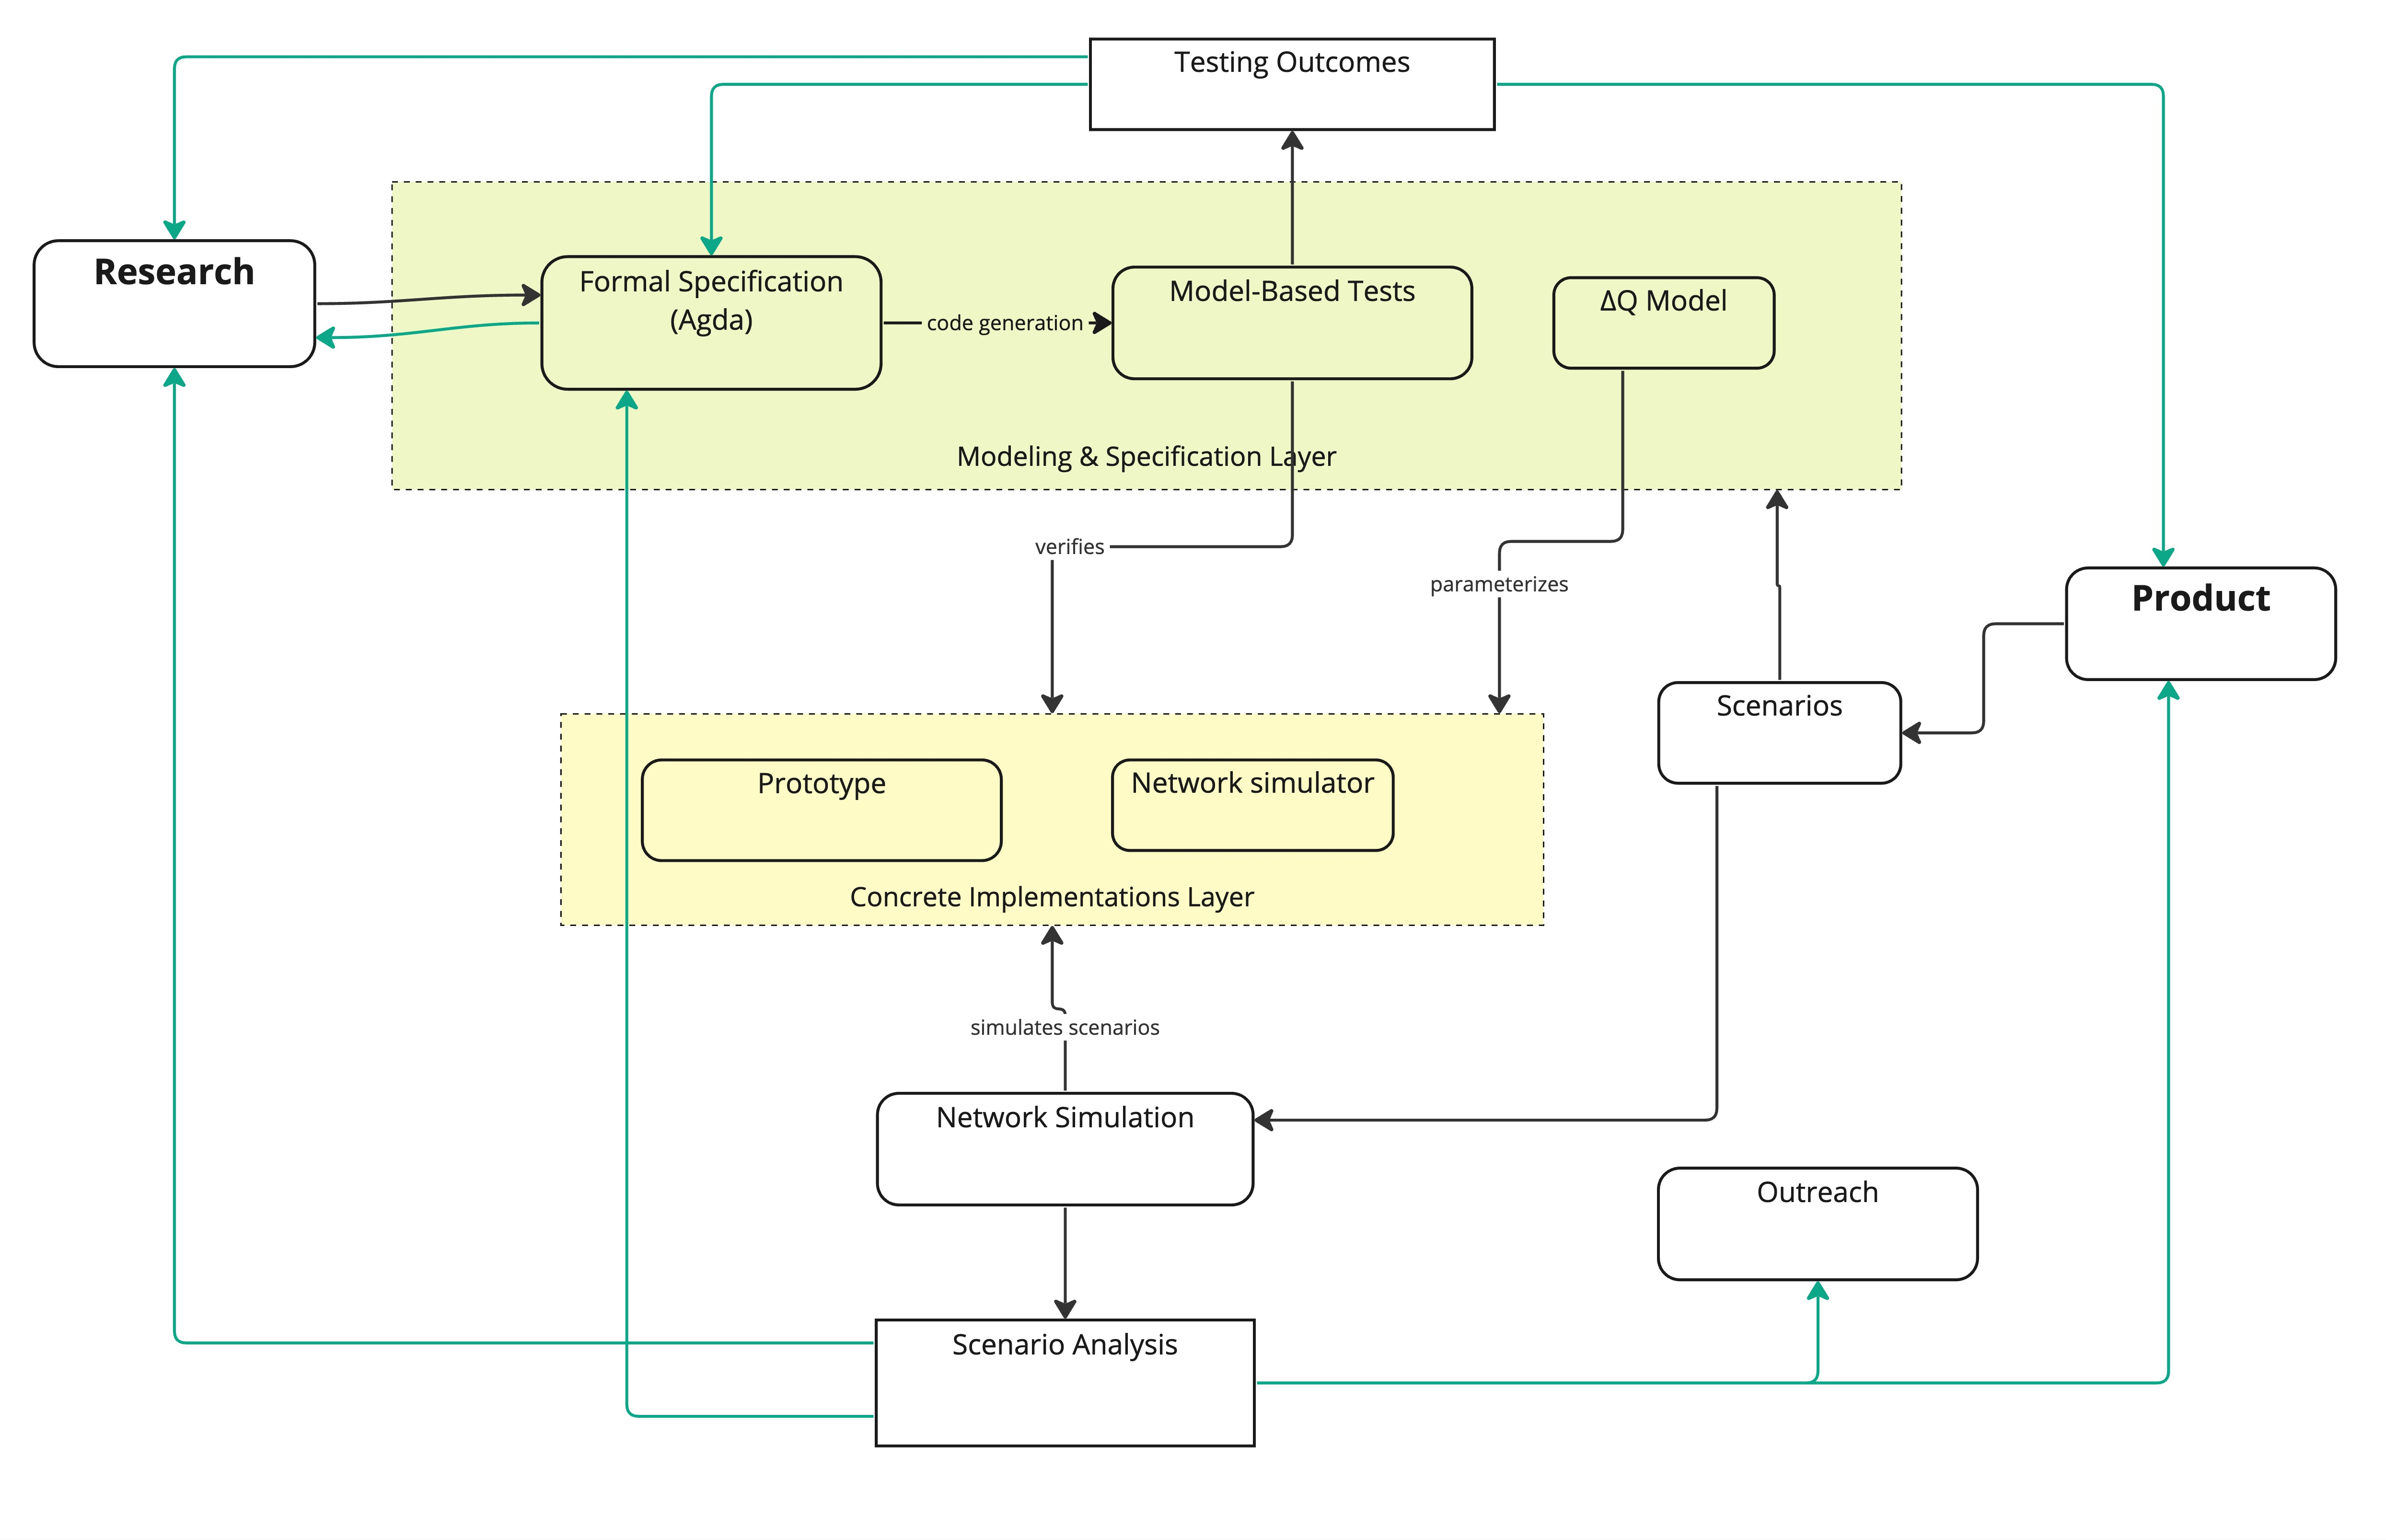
\includegraphics[width=0.80\textwidth]{../diagrams/peras-high-level-architecture.jpg}
\caption{Peras Project Architecture}
\end{figure}

We confirmed the relevance of \hyperref[network-performance-analysis]{ΔQ
modeling} technique to provide insights on a protocol's performance
profile, and how particular design decisions (even apparently minor
ones) can impact this performance profile. We also gave feedback to the
maintainers on the current state of the tool and libraries, and how to
improve it in order to increase the reach of this technique.

We explored the use of formal modeling language Agda to
\hyperref[protocol-specification]{specify} the protocol and application
of Proof-of-Stake-specific \hyperref[small-step-semantics]{proof
techniques} to state and prove relevant properties of the protocol. We
also started work on building a trail of evidence from research to
implementation by:

\begin{itemize}
\tightlist
\item
  Experimenting with Quviq on the
  \hyperref[relating-test-model-to-formal-model]{generation of
  quickcheck-dynamic} test models from Agda models,
\item
  Sketching a research-centric \hyperref[pseudo-code]{\emph{Domain
  Specific Language}} that could be used in research papers and as a
  foundation for formal modeling and engineering work.
\end{itemize}

While prototyping, we demonstrated the applicability of an Agda-centric
chain of evidence even to ``foreign'' languages by testing with
\texttt{quickcheck-dynamic} the same properties against Haskell and
\hyperref[rust-based-simulation]{Rust prototypes}, collaborating with
the Creative engineering team on sketching a
\href{https://github.com/input-output-hk/ce-netsim}{\color{blue}\texttt{network simulator}}
library in Rust.

\subsection{Remaining questions}\label{remaining-questions}

There remain a number of open questions that could be investigated in
future work increments.

\begin{itemize}
\tightlist
\item
  Peras features, both benefits and shortcomings, need to be aligned
  with business cases and overall strategy for scaling Cardano. This
  implies more research is needed in two directions:

  \begin{itemize}
  \tightlist
  \item
    From a product and user perspective, to evaluate the actual value
    that Peras delivers and the possible countermeasures to its
    drawbacks (e.g.~the risk of cool-down could be covered by an
    \emph{options} or \emph{insurance premium} mechanism),
  \item
    From a technical perspective, to explore the parameters space and
    find the best combinations.
  \end{itemize}
\item
  There are a number of components about which we have some ideas but no
  concrete figures or design:

  \begin{itemize}
  \tightlist
  \item
    Certificate structure and capabilities,
  \item
    Vote and certificate CPU requirements and their possible impact on
    the node,
  \item
    Optimal committee size,
  \end{itemize}
\item
  The protocol leaves room for a wide choice of options to design an
  implementation that should be considered and refined,
\item
  There is a need for more theoretical research on ways to make
  cool-down less impactful.
\end{itemize}

\newpage

\section{Previous work}\label{previous-work}

\subsection{Peras workshop}\label{peras-workshop}

A follow-up action from the
\href{https://docs.google.com/document/d/1dv796m2Fc7WH38DNmGc68WOXnqtxj7F30o-kGzM4zKA/edit}{Peras
workshop in Edinburgh}, which happened in September 2023, was to define
a set of questions and experiments to be conducted in order to better
understand the properties of the Peras protocol, along with an
assessment of the protocol's \emph{Software readiness level}. The
following sections recall the questions that were raised during the
workshop, points to the answers given, and details the SRL assessment
along with a comparison with current estimated SRL.

\subsubsection{Questions about Peras}\label{questions-about-peras}

For each of these questions we check whether or not it has been
answered:

\begin{itemize}
\tightlist
\item[$\boxtimes$]
  How do you detect double voting? Is double voting possible? How can
  the voting state be bounded?

  \begin{itemize}
  \tightlist
  \item
    \emph{each vote is signed individually and the signature is checked
    by the receiving node}
  \item
    \emph{the voting state is bound by the committee size and the
    limited validity for each vote}
  \end{itemize}
\item[$\boxtimes$]
  How are the voting committee members selected? What are the properties
  of the voting committee?

  \begin{itemize}
  \tightlist
  \item
    \emph{Committee members are selected by a VRF-based sortition, its
    properties are exposed in the paper and
    \hyperref[overview]{overview}}
  \end{itemize}
\item[$\boxtimes$]
  Where should votes be included: block body, block header, or some
  other aggregate

  \begin{itemize}
  \tightlist
  \item
    \emph{models and simulation show that votes need to be propagated
    and aggregated independently while not in cooldown period}
  \item
    \emph{the ``anchor'' certificate used in cooldown period will need
    to be part of or attached to block bodies while its weight could be
    recorded as part of the corresponding block header}
  \end{itemize}
\item[$\square$]
  Under what circumstance can a cool down be entered?

  \begin{itemize}
  \tightlist
  \item
    \emph{The question of how much adversarial power is needed to
    trigger a cool-down period is still open}
  \end{itemize}
\item[$\boxtimes$]
  How significant is the risk of suppressing votes to trigger a
  cool-down period?

  \begin{itemize}
  \tightlist
  \item
    \emph{it is significant, as being able to trigger cool-downs often
    ruins the benefits of Peras}
  \end{itemize}
\item[$\square$]
  Should vote contributions be incentivized?

  \begin{itemize}
  \tightlist
  \item
    \emph{this question has not been explored in this report}
  \end{itemize}
\item[$\boxtimes$]
  How much weight is added per round of voting?

  \begin{itemize}
  \tightlist
  \item
    \emph{This is a parameter \(B\) in the protocol whose exact value
    depends on business requirements}
  \end{itemize}
\item[$\square$]
  How to expose the weight/settlement of a block to a consumer of chain
  data, such as a wallet?

  \begin{itemize}
  \tightlist
  \item
    \emph{This has not been addressed yet, as most of the user-facing
    and business domain aspects of the protocol}
  \end{itemize}
\item[$\boxtimes$]
  Can included votes be aggregated into an artifact to prove the
  existence of votes \& the weight they provide?

  \begin{itemize}
  \tightlist
  \item
    \emph{This is the role of certificates}
  \end{itemize}
\end{itemize}

\subsubsection{Potential experiments for
Peras}\label{potential-experiments-for-peras}

We refer the reader to the relevant section for each of those potential
experiments to demonstrate (in)feasability of Peras:

\begin{itemize}
\tightlist
\item[$\boxtimes$]
  Network traffic simulation of vote messages

  \begin{itemize}
  \tightlist
  \item
    \emph{This has been \hyperref[simulations]{simulated} but needs to
    be refined}
  \end{itemize}
\item[$\boxtimes$]
  Protocol formalization \& performance simulations of Peras

  \begin{itemize}
  \tightlist
  \item
    \emph{This has been done in \hyperref[agda-specification]{Agda} with
    (parts of) performance modeling using
    \hyperref[network-performance-analysis]{ΔQ} and simulation}
  \end{itemize}
\item[$\boxtimes$]
  Optimal look-back parameter (measured in number of slots) within a
  round

  \begin{itemize}
  \tightlist
  \item[$\square$]
    \emph{Historic analytical study (\(n\)-\(\sigma\) for reliability
    based on the number of 9s desired)}
  \item[$\boxtimes$]
    \emph{Some parameters value are provided in the research paper and
    \href{https://docs.google.com/presentation/d/1QGCvDoOJIWug8jJgCNv3p9BZV-R8UZCyvosgNmN-lJU/edit\#slide=id.g2ca1209fec0_0_450}{\color{blue}\texttt{slides}}}
  \end{itemize}
\item[$\square$]
  Chain growth simulations for the accumulation of vote data

  \begin{itemize}
  \tightlist
  \item
    \emph{This has not been done as the protocol has evolved since the
    workshop}
  \end{itemize}
\item[$\boxtimes$]
  Added chain catch-up time

  \begin{itemize}
  \tightlist
  \item
    \emph{This is cool-down period length and is estimated in the
    \href{https://docs.google.com/presentation/d/1QGCvDoOJIWug8jJgCNv3p9BZV-R8UZCyvosgNmN-lJU/edit\#slide=id.g2ca1209fec0_0_450}{\color{blue}\texttt{slides}}}
  \end{itemize}
\item[$\square$]
  Cost of diffusing votes and blocks that contain votes

  \begin{itemize}
  \tightlist
  \item
    \emph{not estimated}
  \end{itemize}
\item[$\square$]
  Need to refine: Details of VRF-based committee selection and its size
\end{itemize}

\subsubsection{SRL}\label{srl}

SRL (software readiness level) was initially assessed to be between 1
and 2, with the following definitions:

\begin{longtable}[]{@{}
  >{\raggedright\arraybackslash}p{(\columnwidth - 2\tabcolsep) * \real{0.8000}}
  >{\raggedright\arraybackslash}p{(\columnwidth - 2\tabcolsep) * \real{0.2000}}@{}}
\toprule\noalign{}
\begin{minipage}[b]{\linewidth}\raggedright
Questions to resolve
\end{minipage} & \begin{minipage}[b]{\linewidth}\raggedright
Status
\end{minipage} \\
\midrule\noalign{}
\endhead
\bottomrule\noalign{}
\endlastfoot
A concept formulated? & Done \\
Basic scientific principles underpinning the concept identified? &
Done \\
Basic properties of algorithms, representations \& concepts defined? &
Done \\
Preliminary analytical studies confirm the basic concept? & \\
Application identified? & Done (Partner chains) \\
Preliminary design solution identified? & Partial \\
Preliminary system studies show the application to be feasible? & \\
Preliminary performance predictions made? & Done \\
Basic principles coded? & \\
Modeling \& Simulation used to refine performance predictions further
and confirm benefits? & \\
Benefits formulated? & \\
Research \& development approach formulated? & Done \\
Preliminary definition of Laboratory tests and test environments
established? & Preliminary \\
Experiments performed with synthetic data? & \\
Concept/application feasibility \& benefits reported in paper & \\
\end{longtable}

We assess the current SRL to be between 3 and 4, given the following
\href{https://input-output.atlassian.net/wiki/spaces/CI/pages/3875110920/SRL+3+Analytical+and+or+experimental+critical+function+or+characteristic+proof-of-concept.}{SRL
3} definition:

\begin{longtable}[]{@{}
  >{\raggedright\arraybackslash}p{(\columnwidth - 2\tabcolsep) * \real{0.9250}}
  >{\raggedright\arraybackslash}p{(\columnwidth - 2\tabcolsep) * \real{0.0750}}@{}}
\toprule\noalign{}
\begin{minipage}[b]{\linewidth}\raggedright
Questions to resolve
\end{minipage} & \begin{minipage}[b]{\linewidth}\raggedright
Status
\end{minipage} \\
\midrule\noalign{}
\endhead
\bottomrule\noalign{}
\endlastfoot
Critical functions/components of the concept/application identified? &
Done \\
Subsystem or component analytical predictions made? & Partial \\
Subsystem or component performance assessed by Modeling and Simulation?
& Partial \\
Preliminary performance metrics established for key parameters? &
Done \\
Laboratory tests and test environments established? & Done \\
Laboratory test support equipment and computing environment completed
for component/proof-of-concept testing? & N/A \\
Component acquisition/coding completed? & No \\
Component verification and validation completed? & Partial \\
Analysis of test results completed establishing key performance metrics
for components/ subsystems? & Done \\
Analytical verification of critical functions from proof-of-concept
made? & Done \\
Analytical and experimental proof-of-concept documented? & Done \\
\end{longtable}

\section{Protocol specification}\label{protocol-specification}

\subsection{Overview}\label{overview}

A presentation of the motivation and principles of the protocol is
available in these
\href{https://docs.google.com/presentation/d/1QGCvDoOJIWug8jJgCNv3p9BZV-R8UZCyvosgNmN-lJU/edit}{\color{blue}\texttt{slides}}.
We summarize the main points here but refer the interested reader to the
slides and the research article for details.

\begin{itemize}
\tightlist
\item
  Peras adds a Voting layer on top of Praos, Cardano's Nakamoto-style
  consensus protocol.
\item
  In every voting round, stakeholders (SPOs) get selected to be part of
  the voting committee through a stake-based sortition mechanism (using
  their existing VRF keys) and vote for the newest block at least \(L\)
  slots old, where \(L\) is a parameter of the construction (e.g., \(L\)
  = 120 slots).
\item
  Votes are broadcast to other nodes through network diffusion.
\item
  If a block gains more than a certain threshold of votes (from the same
  round), a so-called \emph{quorum} (\(\tau\)), it gets extra weight
  \(B\) (where each block has a base weight of 1). Since nodes always
  select the heaviest chain (as opposed to the longest chain in Praos),
  these blocks with extra weight accelerate settlement of all blocks
  before them.
\item
  A set of votes (from the same round) can be turned into a short
  certificate. Certificates are needed during the cool-down period (see
  below), but they can also be broadcast to nodes that are catching up.
\item
  If a quorum is not reached in a round, the protocol enters a cool-down
  period, in order to heal from the ``damage'' that could result from
  adversarial strategies centered around withholding adversarial votes.
  During the cool-down, voting is suspended, and block producers include
  information required to coordinate the restart (the latest known
  certificate) in their blocks. The duration of the cool-down period is
  roughly equal to the number of slots equivalent to produce \emph{k} +
  \emph{B} blocks, where \emph{k} is the settlement parameter of Praos.
\end{itemize}

\subsubsection{Certificates}\label{certificates}

The exact construction of Peras certificates is still unknown but we
already know the feature set it should provide:

\begin{itemize}
\tightlist
\item
  A Peras certificate must be reasonably ``small'' in order to fit
  within the limits of a single block without leading to increased
  transmission delay.

  \begin{itemize}
  \tightlist
  \item
    The current block size on \texttt{mainnet} is 90kB, with each
    transaction limited to 16kB.
  \item
    In order to not clutter the chain and take up too much block estate,
    a certificate should fit in a \emph{single transaction}.
  \end{itemize}
\item
  Certificates need to be produced \emph{locally} by a single node from
  the aggregation of multiple votes reaching a quorum.

  \begin{itemize}
  \tightlist
  \item
    Certificate forging should be reasonably fast but is not critical
    for block diffusion: A round spans multiple possible blocks so there
    is more time to produce and broadcast it.
  \end{itemize}
\item
  A certificate must be reasonably fast to verify as it is on the
  critical path of chain selection: When a node receives a new block
  and/or a new certificate, it needs to decide whether or not this
  changes its best chain according to the weight,
\item
  The
  \href{https://iohk.io/en/research/library/papers/approximate-lower-bound-arguments/}{\color{blue}\texttt{ALBA}}
  paper provides a construction through a mechanism called a
  \emph{Telescope} which seems like a good candidate for Peras
  certificates.
\end{itemize}

\subsection{Pseudo-code}\label{pseudo-code}

We initially started working from researchers' pseudo-code which was
detailed in various documents:

\begin{itemize}
\tightlist
\item
  The initial
  \href{https://docs.google.com/document/d/1QMn1CqS4zSbKzvozhcAtc7MN_nMfVHhP25pMTxyhhZ8/edit\#heading=h.8bsvt41k7bj1}{protocol
  definition} as presented in the Edinburgh workshop, in September 2023,
\item
  The
  \href{https://docs.google.com/document/d/1lywi65s1nQpAGgMpzPXD-sLzYNES-FZ8SHXF75VCKuI/edit\#heading=h.dqvlvyqlb2s4}{post-workshop
  definition} which considered votes and blocks diffusion and chain
  selection in a more integrated manner,
\item
  The newest version from
  \href{https://docs.google.com/document/d/1w_jHsojcBxZHgGrr63ZGa4nhkgEpkL6a2cFYiq8Vf8c/edit}{March
  2024} which addressed the shortcomings of tallying individual votes in
  the chain selection process from earlier versions.
\end{itemize}

In the Paris Workshop in April 2024, we tried to address a key issue of
this pseudo-code: The fact it lives in an unstructured and informal
document, is not machine-checkable, and is therefore poised to be
quickly out of the sync with both the R\&D work on the formal
specification, the prototyping work, and the research work. This
collective effort led to writing the exact same pseudo-code as a
\emph{literate Agda} document, the internal consistency of which can be
checked by the Agda compiler, while providing a similar level of
flexibility and readability than the original document.

This document is available in the
\href{../../src/Peras/ProtocolL.lagda.md}{\color{blue}\texttt{Peras repository}} and is a
first step towards better integration between research and engineering
work streams.

Next steps include:

\begin{itemize}
\tightlist
\item
  Refining the pseudo-code's syntax to make it readable and maintainable
  by researchers and engineers alike,
\item
  Understanding how this code relates with the actual Agda code,
\item
  Adding some semantics.
\end{itemize}

It is envisioned that at some point this kind of code could become
commonplace in the security researchers community in order to provide
formally verifiable and machine-checkable specifications, based on the
theoretical framework used by researchers (e.g.~Universal Composition).

\subsection{Settlement time}\label{settlement-time}

\href{https://eprint.iacr.org/2022/1571.pdf}{Practical Settlement Bounds
for Longest-Chain Consensus} \emph{(Gazi, Ren, and Russell, 2023)}
provides a formal treatment of the settlement guarantees for
proof-of-stake (PoS) blockchains.

\emph{Settlement time} can be defined as the time needed for a given
transaction to be considered permanent by some honest party. On Cardano,
the upper bound for settlement time is \(3k / f\) to produce \(k\)
subsequent blocks, where \(k\) is the \emph{security parameter} and
\(f\) is the \emph{active slot coefficient}. On the current mainchain,
this time is 36 hours. Note that even if in practice the settlement time
is fixed, in theory this bound is always probabilistic. The security
parameter \(k\) is chosen in such a way that the probability of a
transaction being reverted after \(k\) blocks is lower than
\(10^{-60}\).

The following picture from the aforementioned paper shows block
settlement failure probability given some block depth for Cardano PoS
chain. Under the assumptions given there, the probability for a
transaction to be rolled back after 20 blocks is 0.001\% , and is
exponentially decreasing with the block depth.

\begin{figure}
\centering
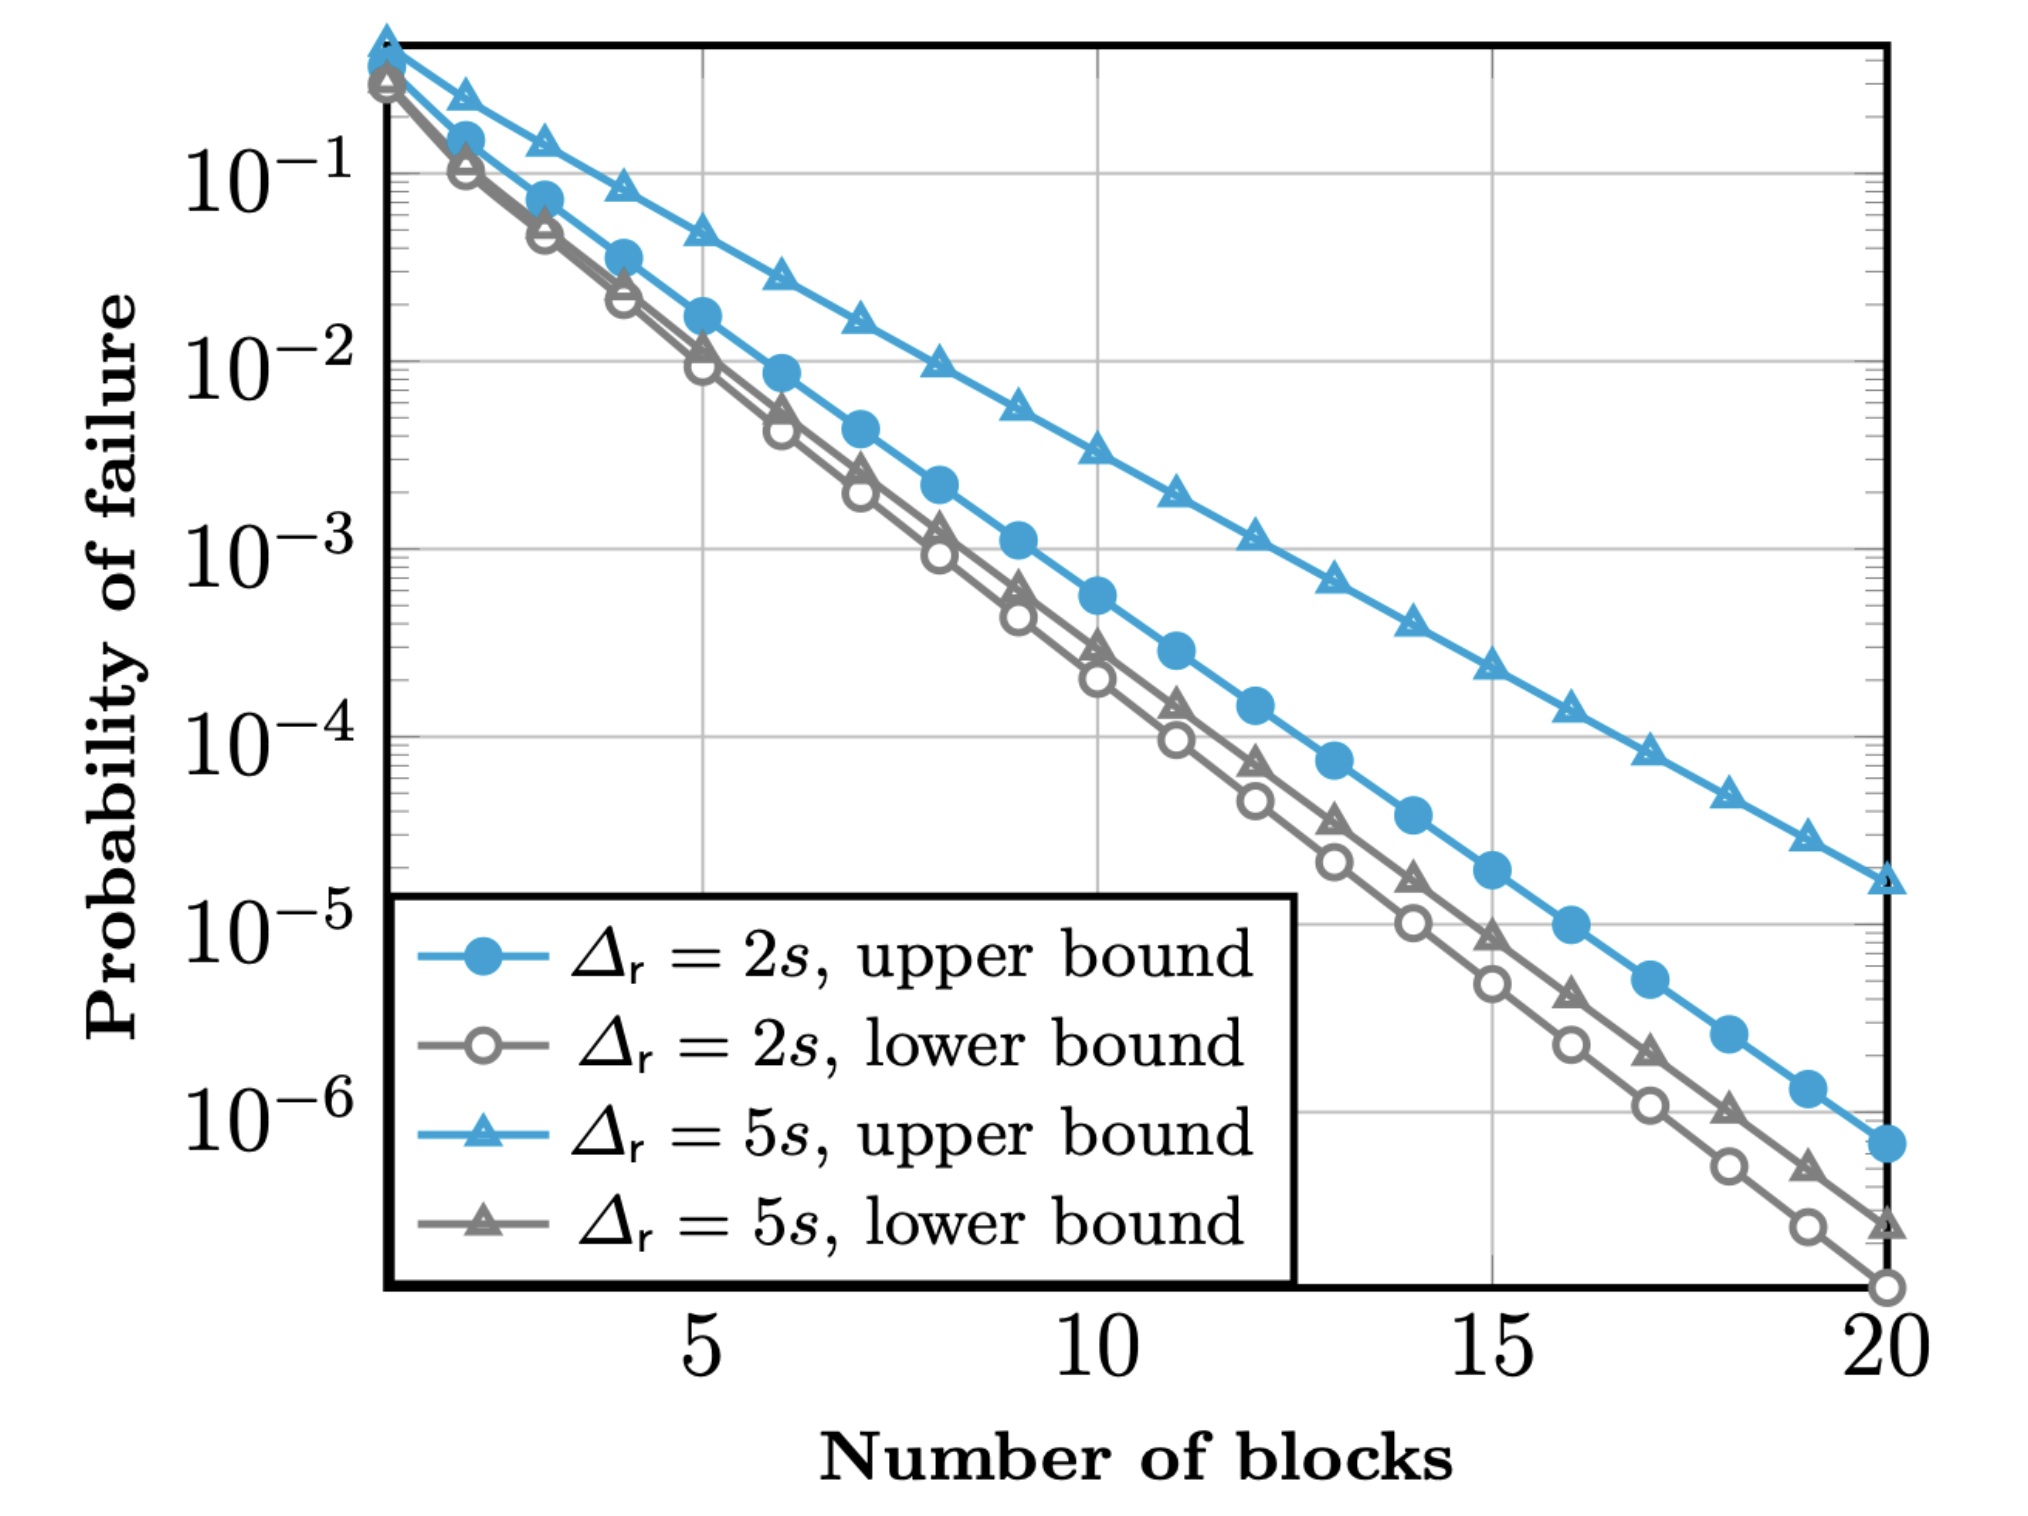
\includegraphics[width=0.48\textwidth]{../diagrams/settlement-failure-probability.png}
\caption{Settlement failure probability / depth for 10\% adversary}
\end{figure}

We also have anecdotal evidence from observations of the Cardano
mainchain over the past few years that the settlement time is much
shorter than the theoretical bound, as basically forks over 2 blocks
length are exceedingly rare, and no fork over 3 blocks length has been
observed on core nodes since the launch of Shelley.

There's however no evidence this situation will continue in the future,
obviously, as it could very well be the case the network was never
seriously under attack, hence we should take those numbers with caution.

\subsubsection{Settlement bounds for
Peras}\label{settlement-bounds-for-peras}

\begin{quoting}
{\emph Take the following analysis with a grain of salt as the researchers are
still actively working on the protocol's security properties and numeric
analysis.}
\end{quoting}

While these numbers seem comforting and reasonably small to provide a
very high degree of confidence after less than 10 minutes (a block is
produced on average every 20s), it should be noted that they are based
on non-existent to low adversarial power assumption (e.g.~lower than
10\% total stake), in other words they represent the best case scenario
and say nothing about the potential impact of an adversary with
significant resources and high motivation to either disrupt the network,
e.g.~as a form of denial of service to degrade the perceived value of
Cardano, or more obviously to double spend. As the stakes increase and
the network becomes more valuable, the probability of such an attack
increases and our confidence in the settlement time should be adjusted
accordingly.

In the optimistic case, Peras is expected to provide the level of
settlement Praos provides after \(k\) blocks but after only about a few
rounds of voting. With the following parameters:

\begin{itemize}
\tightlist
\item
  Committee size \(\cal{S}\) = 2000,
\item
  Boost per certificate \(B = k / 10 = 216\),
\item
  Quorum \(\tau = 3\cal{S} / 4 = 1500\),
\item
  Round length \(U = 10\) slots.
\end{itemize}

we can expect a negligible (\(< 10^{-60}\)) probability of settlement
failure after 10 rounds or 100 slots, which is less than 2 minutes. In
other words, Peras improves settlement upper bound over Praos by a
factor of 1000, in the \emph{optimistic case}, e.g.~outside of a
\emph{cool-down period}.

However, triggering cool-down is cheap and does not require a large
adversarial power as it is enough for an adversary to be able to create
a relatively short fork that lasts slightly longer than the length of
the voting window (\(L\)) to be able to force a split vote and a
cool-down period.

\subsection{Agda specification}\label{agda-specification}

The formal specification of the Peras protocol is implemented in Agda.
It is a declarative specification, there are entities that are only
defined by properties rather than by an explicit implementation. But
still the specification is extractable to Haskell and allows to generate
QuickCheck tests for checking an arbitrary implementation against the
reference specification.

\subsubsection{Domain model}\label{domain-model}

\textbf{Note}: The code here is substantially different from the
\hyperref[pseudo-code]{pseudo-code} mentioned before. These represent
two different lines of work that ultimately should be reconciled.

The domain model is defined as Agda data types and implemented with
Haskell code extraction in mind. The extractable domain model comprises
entities like \texttt{Block}, \texttt{Chain}, \texttt{Vote} or
\texttt{Certificate}. For example the Agda record type for
\texttt{Block}

\begin{Shaded}
\begin{Highlighting}[]
\KeywordTok{record}\NormalTok{ Block }\KeywordTok{where}
  \KeywordTok{field}\NormalTok{ slotNumber }\OtherTok{:}\NormalTok{ Slot}
\NormalTok{        creatorId }\OtherTok{:}\NormalTok{ PartyId}
\NormalTok{        parentBlock }\OtherTok{:}\NormalTok{ Hash Block}
\NormalTok{        certificate }\OtherTok{:}\NormalTok{ Maybe Certificate}
\NormalTok{        leadershipProof }\OtherTok{:}\NormalTok{ LeadershipProof}
\NormalTok{        signature }\OtherTok{:}\NormalTok{ Signature}
\NormalTok{        bodyHash }\OtherTok{:}\NormalTok{ Hash }\OtherTok{(}\NormalTok{List Tx}\OtherTok{)}
\end{Highlighting}
\end{Shaded}

is extracted to the Haskell data type:

\begin{Shaded}
\begin{Highlighting}[]
\KeywordTok{data} \DataTypeTok{Block} \OtherTok{=} \DataTypeTok{Block}
\NormalTok{  \{}\OtherTok{ slotNumber ::} \DataTypeTok{Slot}
\NormalTok{  ,}\OtherTok{ creatorId ::} \DataTypeTok{PartyId}
\NormalTok{  ,}\OtherTok{ parentBlock ::} \DataTypeTok{Hash} \DataTypeTok{Block}
\NormalTok{  ,}\OtherTok{ certificate ::} \DataTypeTok{Maybe} \DataTypeTok{Certificate}
\NormalTok{  ,}\OtherTok{ leadershipProof ::} \DataTypeTok{LeadershipProof}
\NormalTok{  ,}\OtherTok{ signature ::} \DataTypeTok{Signature}
\NormalTok{  ,}\OtherTok{ bodyHash ::} \DataTypeTok{Hash}\NormalTok{ [}\DataTypeTok{Tx}\NormalTok{]}
\NormalTok{  \}}
  \KeywordTok{deriving}\NormalTok{ (}\DataTypeTok{Eq}\NormalTok{)}
\end{Highlighting}
\end{Shaded}

Cryptographic functions are not implemented in the specification. For
example, for hash functions there is the record type \texttt{Hashable}

\begin{Shaded}
\begin{Highlighting}[]
\KeywordTok{record}\NormalTok{ Hashable }\OtherTok{(}\NormalTok{a }\OtherTok{:} \DataTypeTok{Set}\OtherTok{)} \OtherTok{:} \DataTypeTok{Set} \KeywordTok{where}
  \KeywordTok{field}\NormalTok{ hash }\OtherTok{:}\NormalTok{ a }\OtherTok{→}\NormalTok{ Hash a}
\end{Highlighting}
\end{Shaded}

that is extracted to a corresponding type class in Haskell:

\begin{Shaded}
\begin{Highlighting}[]
\KeywordTok{class} \DataTypeTok{Hashable}\NormalTok{ a }\KeywordTok{where}
\OtherTok{  hash ::}\NormalTok{ a }\OtherTok{{-}\textgreater{}} \DataTypeTok{Hash}\NormalTok{ a}
\end{Highlighting}
\end{Shaded}

For executing the reference specification, an instance of the different
kind of hashes (for example for hashing blocks) needs to be provided.

\paragraph{Agda2hs}\label{agda2hs}

In order to generate ``readable'' Haskell code, we use
\href{https://agda.github.io/agda2hs}{\color{blue}\texttt{agda2hs}} rather than relying on
the standard Haskell generator code (\texttt{MAlonzo}) directly. It
happens that \texttt{agda2hs} is not compatible with the Agda standard
library and therefore we are using the custom \texttt{Prelude} provided
by \texttt{agda2hs} that is also extractable to Haskell.

For extracting properties from Agda to Haskell we can use a similar type
as the \texttt{Equal} type from the \texttt{agda2hs} examples. The
constructor for \texttt{Equal} takes a pair of items and a proof that
those are equal. When extracting to Haskell the proof gets erased. We
can use this idea for extracting properties to be used with quick-check.

\begin{Shaded}
\begin{Highlighting}[]
\NormalTok{prop{-}genesis{-}in{-}slot0 }\OtherTok{:} \OtherTok{∀} \OtherTok{\{}\NormalTok{c }\OtherTok{:}\NormalTok{ Chain}\OtherTok{\}} \OtherTok{→} \OtherTok{(}\NormalTok{v }\OtherTok{:}\NormalTok{ ValidChain c}\OtherTok{)} \OtherTok{→}\NormalTok{ slot }\OtherTok{(}\NormalTok{last c}\OtherTok{)}\NormalTok{ ≡ }\DecValTok{0}
\NormalTok{prop{-}genesis{-}in{-}slot0 }\OtherTok{=} \OtherTok{...}

\NormalTok{propGenesisInSlot0 }\OtherTok{:} \OtherTok{∀} \OtherTok{(}\NormalTok{c }\OtherTok{:}\NormalTok{ Chain}\OtherTok{)} \OtherTok{→} \OtherTok{(@}\DecValTok{0}\NormalTok{ v }\OtherTok{:}\NormalTok{ ValidChain c}\OtherTok{)} \OtherTok{→}\NormalTok{ Equal ℕ}
\NormalTok{propGenesisInSlot0 c v }\OtherTok{=}\NormalTok{ MkEqual }\OtherTok{(}\NormalTok{slot }\OtherTok{(}\NormalTok{last c}\OtherTok{)}\NormalTok{ , }\DecValTok{0}\OtherTok{)} \OtherTok{(}\NormalTok{prop{-}genesis{-}in{-}slot0 v}\OtherTok{)}
\end{Highlighting}
\end{Shaded}

\subsubsection{Small-step semantics}\label{small-step-semantics}

In order to describe the execution of the protocol, we are proposing a
\href{../../src/Peras/SmallStep.lagda.md}{small-step semantics for
Ouroboros Peras} in Agda based on ideas from the small-step semantics
for Ouroboros Praos as laid out in the PoS-NSB paper. The differences in
the small-step semantics of the Ouroboros Praos part of the protocol are
explained in the following sections.

\paragraph{Local state}\label{local-state}

The local state is the state of a single party, respectively a single
node. It consists of a declarative \emph{blocktree}, i.e.~an abstract
data structure representing possible chains specified by a set of
properties. In addition to blocks, the blocktree for Ouroboros, Peras
also includes votes and certificates and for this reason there are
additional properties with respect to those entities.

The fields of the blocktree allow to:

\begin{itemize}
\tightlist
\item
  Extend the tree with blocks and votes,
\item
  Get all blocks, votes and certificates,
\item
  Get the best chain.
\end{itemize}

The property stating that the best chain is always a valid chain is such
a property:

\begin{Shaded}
\begin{Highlighting}[]
\NormalTok{valid }\OtherTok{:} \OtherTok{∀} \OtherTok{(}\NormalTok{t }\OtherTok{:}\NormalTok{ tT}\OtherTok{)} \OtherTok{(}\NormalTok{sl }\OtherTok{:}\NormalTok{ Slot}\OtherTok{)}
  \OtherTok{→}\NormalTok{ ValidChain }\OtherTok{(}\NormalTok{bestChain sl t}\OtherTok{)}
\end{Highlighting}
\end{Shaded}

The condition which chain is considered the best is given by the
following property:

\begin{Shaded}
\begin{Highlighting}[]
\NormalTok{optimal }\OtherTok{:} \OtherTok{∀} \OtherTok{(}\NormalTok{c }\OtherTok{:}\NormalTok{ Chain}\OtherTok{)} \OtherTok{(}\NormalTok{t }\OtherTok{:}\NormalTok{ tT}\OtherTok{)} \OtherTok{(}\NormalTok{sl }\OtherTok{:}\NormalTok{ Slot}\OtherTok{)}
  \OtherTok{→} \KeywordTok{let}\NormalTok{ b }\OtherTok{=}\NormalTok{ bestChain sl t}
    \KeywordTok{in}
\NormalTok{    ValidChain c}
  \OtherTok{→}\NormalTok{ c ⊆ allBlocksUpTo sl t}
  \OtherTok{→}\NormalTok{ weight c }\OtherTok{(}\NormalTok{certs t c}\OtherTok{)}\NormalTok{ ≤ weight b }\OtherTok{(}\NormalTok{certs t b}\OtherTok{)}
\end{Highlighting}
\end{Shaded}

In words, this says that the \emph{best} chain is \emph{valid}
(\texttt{ValidChain} is a predicate asserting that a chain is valid with
respect to Ouroboros Praos) and the \emph{heaviest} chain out of all
valid chains is the best.

\paragraph{Global state}\label{global-state}

In order to describe progress with respect to the Ouroboros Peras
protocol, a global state is introduced. The global state consists of the
following entities:

\begin{itemize}
\tightlist
\item
  \emph{clock:} Keeps track of the current slot of the system.
\item
  \emph{state map:} Map storing local state per party, i.e.~the
  blocktrees of all the nodes.
\item
  \emph{messages:} All the messages that have been sent but not yet
  delivered.
\item
  \emph{history:} All the messages that have been sent.
\item
  \emph{adversarial state:} The adversarial state can be anything, with
  the type is passed to the specification as a parameter.
\end{itemize}

The differences compared to the model proposed in the PoS-NSB paper are:

\begin{itemize}
\tightlist
\item
  the execution order is not stored in the global state and therefore
  permutations of the messages as well as permutations of parties are
  not needed,
\item
  the \texttt{Progress} of the system as described in the PoS-NSB paper
  is not stored in the global state, as we define the global relation
  more granular
\end{itemize}

Instead of keeping track of the execution order of the parties in the
global state, the global relation is defined with respect to parties.
The list of parties is considered fixed from the beginning and passed to
the specification as a parameter. Together with a party, we know as well
the party's honesty (\texttt{Honesty} is a predicate for a party).
Instead of keeping track of progress globally we only need to assert
that before the clock reaches the next slot, all the deliverable
messages (i.e.~messages where the delay is 0) in the global message
buffer have been consumed.

\paragraph{Global relation}\label{global-relation}

The protocol defines messages to be distributed between parties of the
system. The specification currently implements the following message
types:

\begin{itemize}
\tightlist
\item
  \emph{Block message:} When a party is the slot leader a new block can
  be created and a message notifying the other parties about the block
  creation is broadcast. Note that, in case a cool-down phase according
  to the Ouroboros Peras protocol is detected, the block also includes a
  certificate that references a block of the party's preferred chain,
\item
  \emph{Vote message:} When a party creates a vote according to the
  protocol, this is wrapped into a message and delivered to the other
  parties.
\end{itemize}

The global relation expresses the evolution of the global state:

\begin{Shaded}
\begin{Highlighting}[]
    \KeywordTok{data} \OtherTok{\_}\NormalTok{↝}\OtherTok{\_} \OtherTok{:}\NormalTok{ Stateᵍ }\OtherTok{→}\NormalTok{ Stateᵍ }\OtherTok{→} \DataTypeTok{Set} \KeywordTok{where}

\NormalTok{      Deliver }\OtherTok{:} \OtherTok{∀} \OtherTok{\{}\NormalTok{M N p}\OtherTok{\}} \OtherTok{\{}\NormalTok{h }\OtherTok{:}\NormalTok{ Honesty p}\OtherTok{\}} \OtherTok{\{}\NormalTok{m}\OtherTok{\}}
        \OtherTok{→}\NormalTok{ h ⊢ M [ m ]⇀ N}
          \CommentTok{{-}{-}{-}{-}{-}{-}{-}{-}{-}{-}{-}{-}{-}{-}}
        \OtherTok{→}\NormalTok{ M ↝ N}

\NormalTok{      CastVote }\OtherTok{:} \OtherTok{∀} \OtherTok{\{}\NormalTok{M N p}\OtherTok{\}} \OtherTok{\{}\NormalTok{h }\OtherTok{:}\NormalTok{ Honesty p}\OtherTok{\}}
        \OtherTok{→}\NormalTok{ h ⊢ M ⇉ N}
          \CommentTok{{-}{-}{-}{-}{-}{-}{-}{-}{-}}
        \OtherTok{→}\NormalTok{ M ↝ N}

\NormalTok{      CreateBlock }\OtherTok{:} \OtherTok{∀} \OtherTok{\{}\NormalTok{M N p}\OtherTok{\}} \OtherTok{\{}\NormalTok{h }\OtherTok{:}\NormalTok{ Honesty p}\OtherTok{\}}
        \OtherTok{→}\NormalTok{ h ⊢ M ↷ N}
          \CommentTok{{-}{-}{-}{-}{-}{-}{-}{-}{-}}
        \OtherTok{→}\NormalTok{ M ↝ N}

\NormalTok{      NextSlot }\OtherTok{:} \OtherTok{∀} \OtherTok{\{}\NormalTok{M}\OtherTok{\}}
        \OtherTok{→}\NormalTok{ Delivered M}
          \CommentTok{{-}{-}{-}{-}{-}{-}{-}{-}{-}{-}{-}}
        \OtherTok{→}\NormalTok{ M ↝ tick M}
\end{Highlighting}
\end{Shaded}

The global relation consists of the following constructors:

\begin{itemize}
\tightlist
\item
  \emph{Deliver}: A party consuming a message from the global message
  buffer is a global state transition. The party might be \emph{honest}
  or \emph{adversarial}, in the latter case a message will be delayed
  rather than consumed,
\item
  \emph{Cast vote}: A vote is created by a party and a corresponding
  message is put into the global message buffer for all parties
  respectively,
\item
  \emph{Create block}: If a party is a slot leader, a new block can be
  created and put into the global message buffer for the other parties.
  In case that a chain according to the Peras protocol enters a
  cool-down phase, the party adds a certificate to the block as well,
\item
  \emph{Next slot}: Allows to advance the global clock by one slot. Note
  that this is only possible, if all the messages for the current slot
  are consumed as expressed by the \texttt{Delivered} predicate.
\end{itemize}

The reflexive transitive closure of the global relation describes what
global states are reachable.

\subsubsection{Proofs}\label{proofs}

The properties and proofs that we can state based upon the formal
specification are in
\href{../../src/Peras/SmallStep/Properties.lagda.md}{\color{blue}\texttt{Properties.lagda.md}}.

A first property is \texttt{knowledge-propagation}, a lemma that states
that knowledge about blocks is propagated between honest parties in the
system. In detail the lemma expresses that for two honest parties the
blocks in the blocktree of the first party will be a subset of the
blocks of the second party after any number of state transitions into a
state where all the messages have been delivered. Or in Agda:

\begin{Shaded}
\begin{Highlighting}[]
\NormalTok{    knowledge{-}propagation }\OtherTok{:} \OtherTok{∀} \OtherTok{\{}\NormalTok{N₁ N₂ }\OtherTok{:}\NormalTok{ GlobalState}\OtherTok{\}}
      \OtherTok{→} \OtherTok{\{}\NormalTok{p₁ p₂ }\OtherTok{:}\NormalTok{ PartyId}\OtherTok{\}}
      \OtherTok{→} \OtherTok{\{}\NormalTok{t₁ t₂ }\OtherTok{:}\NormalTok{ A}\OtherTok{\}}
      \OtherTok{→} \OtherTok{\{}\NormalTok{honesty₁ }\OtherTok{:}\NormalTok{ Honesty p₁}\OtherTok{\}}
      \OtherTok{→} \OtherTok{\{}\NormalTok{honesty₂ }\OtherTok{:}\NormalTok{ Honesty p₂}\OtherTok{\}}
      \OtherTok{→}\NormalTok{ honesty₁ ≡ Honest }\OtherTok{\{}\NormalTok{p₁}\OtherTok{\}}
      \OtherTok{→}\NormalTok{ honesty₂ ≡ Honest }\OtherTok{\{}\NormalTok{p₂}\OtherTok{\}}
      \OtherTok{→} \OtherTok{(}\NormalTok{p₁ , honesty₁}\OtherTok{)}\NormalTok{ ∈ parties}
      \OtherTok{→} \OtherTok{(}\NormalTok{p₂ , honesty₂}\OtherTok{)}\NormalTok{ ∈ parties}
      \OtherTok{→}\NormalTok{ N₀ ↝⋆ N₁}
      \OtherTok{→}\NormalTok{ N₁ ↝⋆ N₂}
      \OtherTok{→}\NormalTok{ lookup }\OtherTok{(}\NormalTok{stateMap N₁}\OtherTok{)}\NormalTok{ p₁ ≡ just ⟪ t₁ ⟫}
      \OtherTok{→}\NormalTok{ lookup }\OtherTok{(}\NormalTok{stateMap N₂}\OtherTok{)}\NormalTok{ p₂ ≡ just ⟪ t₂ ⟫}
      \OtherTok{→}\NormalTok{ Delivered N₂}
      \OtherTok{→}\NormalTok{ clock N₁ ≡ clock N₂}
      \OtherTok{→}\NormalTok{ allBlocks blockTree t₁ ⊆ allBlocks blockTree t₂}
\end{Highlighting}
\end{Shaded}

Knowledge propagation is a pre-requisite for the chain growth property,
it informally states that in each period, the best chain of any honest
party will increase at least by a number that is proportional to the
number of lucky slots in that period, where a lucky slot is any slot
where an honest party is a slot leader.

\section{Network performance
analysis}\label{network-performance-analysis}

We provide in this section the methodology and results of the analysis
of the Peras protocol performance in the context of the Cardano network.
This analysis is not complete as it only covers the impact of including
certificates in block headers, which is not a property of the protocol
anymore. More analysis is needed on the votes and certificates diffusion
process following changes to the protocol in March 2024.

\subsection{Certificates in block
header}\label{certificates-in-block-header}

This section provides high-level analysis of the impact of Peras
protocol on the existing Cardano network, using
\href{https://iohk.io/en/research/library/papers/mind-your-outcomes-the-dqsd-paradigm-for-quality-centric-systems-development-and-its-application-to-a-blockchain-case-study/}{ΔQSD
methodology}. In order to provide a baseline to compare with, we first
applied ΔQ to the existing Praos protocol reconstructing the results
that lead to the current set of parameters defining the performance
characteristics of Cardano, following section 4 of the aforementioned
paper. We then used the same modeling technique taking into account the
Peras protocol \textbf{assuming inclusion of certificates in headers}
insofar as they impact the core \emph{outcome} of the Cardano network,
namely \emph{block diffusion time}.

\begin{quoting}
One of the sub-goals for Peras project is to collaborate
with PNSol, the original inventor of ΔQ methodology, to improve the
usability of the whole method and promote it as a standard tool for
designing distributed systems.
\end{quoting}

\subsubsection{Baseline - Praos ΔQ
modeling}\label{baseline---praos-ux3b4q-modeling}

\paragraph{Model overview}\label{model-overview}

Here is a graphical representation of the \emph{outcome diagram} for the
ΔQ model of Cardano network under Praos protocol:

\begin{figure}
\centering
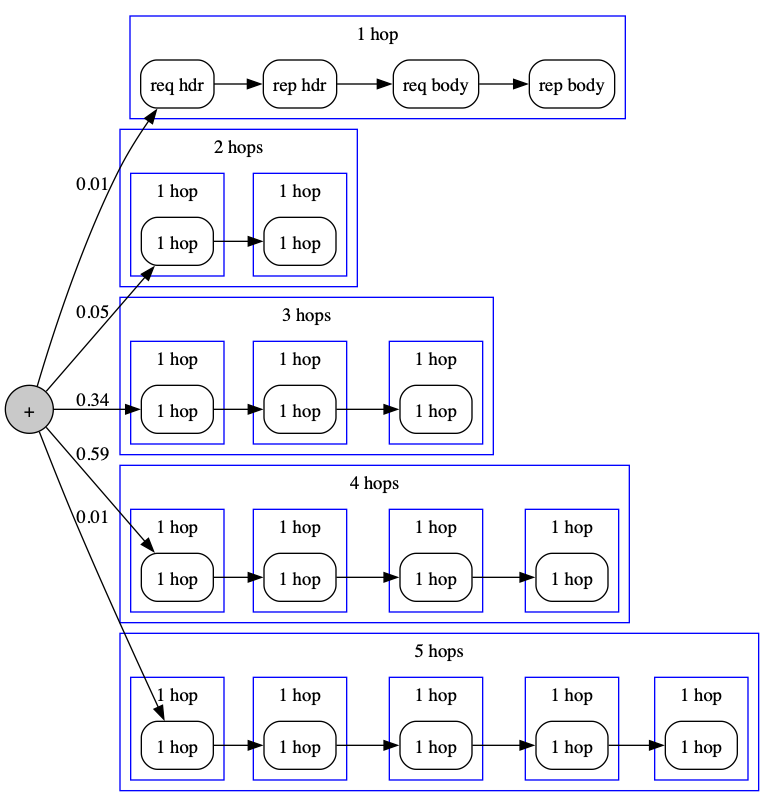
\includegraphics[width=0.48\textwidth]{../diagrams/praos-delta-q.png}
\caption{Outcome diagram for Praos}
\end{figure}

This model is based on the following assumptions:

\begin{itemize}
\tightlist
\item
  Full block diffusion is separated in a number of steps: request and
  reply of the block header, then request and reply of the block body,
\item
  Propagating a block across the network might require several ``hops''
  as there is not a direct connection between every pair of nodes, with
  the distribution of paths length depending on the network topology,
\item
  We have not considered the probability of loss in the current model.
\end{itemize}

The block and body sizes are assumed to be:

\begin{itemize}
\tightlist
\item
  Block header size is smaller than typical MTU of IP network (e.g.~1500
  bytes) and therefore requires a single roundtrip of TCP messages for
  propagation,
\item
  Block body size is about 64kB which implies propagation requires
  several TCP packets sending and therefore takes more time.
\end{itemize}

\begin{quoting}
As the Cardano network uses TCP/IP for its transport, we
should base the header size on the
\href{https://en.wikipedia.org/wiki/Maximum_segment_size}{Maximum
Segment Size}, not the MTU. This size is 536 for IPv4 and 1220 for IPv6.
\end{quoting}

Average latency numbers are drawn from table 1 in the paper and depend
on the (physical) distance between 2 connected nodes:

\begin{longtable}[]{@{}lll@{}}
\toprule\noalign{}
Distance & 1 segment RTT (ms) & 64 kB RTT (ms) \\
\midrule\noalign{}
\endhead
\bottomrule\noalign{}
\endlastfoot
Short & 12 & 24 \\
Medium & 69 & 143 \\
Long & 268 & 531 \\
\end{longtable}

For each step in the diffusion of a block, we assume an equal
(\(\frac{1}{3}\)) chance for each class of distance.

\begin{quoting}
The actual maximum block body size at the time of this
writing is 90kB, but for want of an actual delay value for this size, we
chose the nearest increment available. We need to actually measure the
real value for this block size and other significant increments.
\end{quoting}

We have chosen to define two models of ΔQ diffusion, one based on an
average node degree of 10, and another one on 15. Table 2 gives us the
following distribution of paths length:

\begin{longtable}[]{@{}lll@{}}
\toprule\noalign{}
Length & Degree = 10 & Degree = 15 \\
\midrule\noalign{}
\endhead
\bottomrule\noalign{}
\endlastfoot
1 & 0.40\% & 0.60\% \\
2 & 3.91\% & 8.58\% \\
3 & 31.06\% & 65.86\% \\
4 & 61.85\% & 24.95\% \\
5 & 2.78\% & 0 \\
\end{longtable}

These numbers are reflected (somewhat inaccurately) in the above graph,
representing the probabilities for the number of hops a block will have
to go through before reaching another node.

\begin{quoting}
The current target valency for cardano-node's connection is
20, and while there are a large number of stake pools in operation,
there is some significant concentration of stake, which means the actual
number of ``core'' nodes to consider would be smaller and the
distribution of paths length closer to 1.
\end{quoting}

\paragraph{Modeling process}\label{modeling-process}

We have experimented with three different libraries for encoding this
baseline model:

\begin{enumerate}
\def\labelenumi{\arabic{enumi}.}
\tightlist
\item
  Original \href{https://github.com/DeltaQ-SD/pnsol-deltaq-clone}{ΔQ
  library} built by Neil Davies, which uses randomized sampling to graph
  the \emph{Cumulative Distribution Function} resulting from the ΔQ
  model,
\item
  A library for \href{https://github.com/DeltaQ-SD/Artjoms}{algebraic
  representation} of ΔQ models built to support the
  \href{https://arxiv.org/pdf/2308.10654v1.pdf}{Algebraic Reasoning with
  Timeliness} paper, which uses discretization of probability density
  functions to approximate CFDs resulting from the various ΔQ language
  combinators,
\item
  Another recent library built by Peter Thompson to represent ΔQ
  probability distributions using
  \href{https://github.com/DeltaQ-SD/dqsd-piecewise-poly}{piecewise
  polynomials}, which should provide high-fidelity CDFs.
\end{enumerate}

Library 2 was used to express the \emph{outcome diagram} depicted above
using so-called \emph{O language}, but while we were able to encode the
model itself, the resulting computation of \emph{CDFs} for composite
expressions resulting from \emph{convolution} of atomic expressions
turned out to be unusable, yielding CDFs with accumulated probability
lower than 1 even though we did not model any loss. Library 3, although
the most promising to provide accurate models, turned out to be
unsatisfactory as we were not able to produce proper numerical
representations of a CDF for more complex expressions.

Using code from library 1, we were able to write the following ΔQ
expressions to represent our Cardano model:

\begin{Shaded}
\begin{Highlighting}[]
\NormalTok{oneMTU }\OtherTok{=}
\NormalTok{    fromQTA }\OperatorTok{@}\DataTypeTok{SimpleUniform}
\NormalTok{        [(}\DecValTok{0}\NormalTok{, }\DecValTok{0}\NormalTok{), (}\DecValTok{1} \OperatorTok{\%} \DecValTok{3}\NormalTok{, }\FloatTok{0.012}\NormalTok{), (}\DecValTok{2} \OperatorTok{\%} \DecValTok{3}\NormalTok{, }\FloatTok{0.069}\NormalTok{), (}\DecValTok{3} \OperatorTok{\%} \DecValTok{3}\NormalTok{, }\FloatTok{0.268}\NormalTok{)]}
\NormalTok{blockBody64K }\OtherTok{=}
\NormalTok{    fromQTA }\OperatorTok{@}\DataTypeTok{SimpleUniform}
\NormalTok{        [(}\DecValTok{0}\NormalTok{, }\DecValTok{0}\NormalTok{), (}\DecValTok{1} \OperatorTok{\%} \DecValTok{3}\NormalTok{, }\FloatTok{0.024}\NormalTok{), (}\DecValTok{2} \OperatorTok{\%} \DecValTok{3}\NormalTok{, }\FloatTok{0.143}\NormalTok{), (}\DecValTok{3} \OperatorTok{\%} \DecValTok{3}\NormalTok{, }\FloatTok{0.531}\NormalTok{)]}
\NormalTok{headerRequestReply }\OtherTok{=}\NormalTok{ oneMTU ⊕ oneMTU }\CommentTok{{-}{-} request/reply}
\NormalTok{bodyRequestReply }\OtherTok{=}\NormalTok{ oneMTU ⊕ blockBody64K }\CommentTok{{-}{-} request/reply}
\NormalTok{oneBlockDiffusion }\OtherTok{=}\NormalTok{ headerRequestReply ⊕ bodyRequestReply}

\NormalTok{combine [(p, dq), (\_, dq\textquotesingle{})] }\OtherTok{=}\NormalTok{ (⇋) (}\FunctionTok{toRational} \OperatorTok{$}\NormalTok{ p }\OperatorTok{/} \DecValTok{100}\NormalTok{) dq dq\textquotesingle{}}
\NormalTok{combine ((p, dq) }\OperatorTok{:}\NormalTok{ rest) }\OtherTok{=}\NormalTok{ (⇋) (}\FunctionTok{toRational} \OperatorTok{$}\NormalTok{ p }\OperatorTok{/} \DecValTok{100}\NormalTok{) dq (combine rest)}

\NormalTok{multihops }\OtherTok{=}\NormalTok{ (}\OtherTok{\textasciigrave{}multiHop\textasciigrave{}}\NormalTok{ oneBlockDiffusion) }\OperatorTok{\textless{}$\textgreater{}}\NormalTok{ [}\DecValTok{1} \OperatorTok{..}\NormalTok{]}

\NormalTok{pathLengthsDistributionDegree15 }\OtherTok{=}
\NormalTok{    [}\FloatTok{0.60}\NormalTok{, }\FloatTok{8.58}\NormalTok{, }\FloatTok{65.86}\NormalTok{, }\FloatTok{24.95}\NormalTok{]}
\NormalTok{hopsProba15 }\OtherTok{=} \FunctionTok{zip}\NormalTok{ (}\FunctionTok{scanl1}\NormalTok{ (}\OperatorTok{+}\NormalTok{) pathLengthsDistributionDegree15 }\OperatorTok{\textless{}\textgreater{}}\NormalTok{ [}\DecValTok{0}\NormalTok{]) multihops}
\NormalTok{deltaq15 }\OtherTok{=}\NormalTok{ combine hopsProba15}
\end{Highlighting}
\end{Shaded}

Then computing the empirical CDF over 5000 different random samples
yield the following graph:

\begin{figure}
\centering
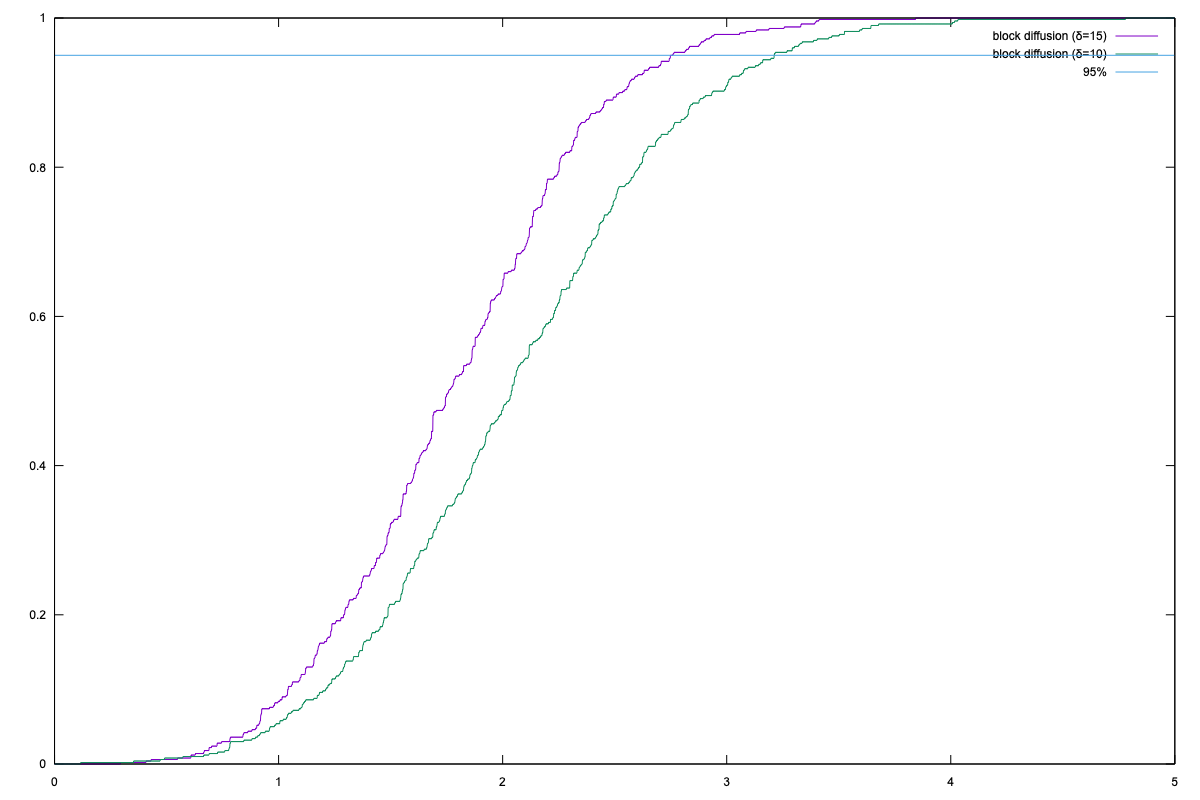
\includegraphics[width=0.68\textwidth]{../diagrams/plot-hops-distribution.png}
\caption{Praos ΔQ Model CDF}
\end{figure}

To calibrate our model, we have computed an empirical distribution of
block adoption time\footnote{This data was kindly provided by
  \href{https://www.linkedin.com/in/markus-gufler}{\color{blue}\texttt{Markus Gufler}}}
observed on the \texttt{mainnet} over the course of 4 weeks (from 22nd
February 2024 to 18th March 2024), as provided by
https://api.clio.one/blocklog/timeline/. The raw data is provided as a
file with 12 millions entries similar to:

\begin{verbatim}
9963861,117000029,57.128.141.149,192.168.1.1,570,0,60,30
9963861,117000029,57.128.141.149,192.168.1.1,540,0,60,40
9963861,117000029,158.101.97.195,150.136.84.82,320,0,10,50
9963861,117000029,185.185.82.168,158.220.80.17,610,0,50,50
9963861,117000029,74.122.122.114,10.10.100.12,450,0,10,50
9963861,117000029,69.156.16.141,69.156.16.141,420,0,10,50
9963861,117000029,165.227.139.87,10.114.0.2,620,10,0,70
9963861,117000029,192.99.4.52,144.217.78.44,460,0,10,100
9963861,117000029,49.12.89.235,135.125.188.228,550,0,20,50
9963861,117000029,168.119.9.11,3.217.90.52,450,150,10,50
...
\end{verbatim}

Each entry provides:

\begin{itemize}
\tightlist
\item
  Block height,
\item
  Slot number,
\item
  Emitter and receiver's IP addresses,
\item
  Time (in ms) to header announcement,
\item
  then additional time to fetch header,
\item
  time to download block,
\item
  and finally time to adopt a block on the receiver.
\end{itemize}

Therefore the total time for block diffusion is the sum of the last 4
columns.

This data is gathered through a network of over 100 collaborating nodes
that agreed to report various statistics to a central aggregator, so it
is not exhaustive and could be biased. The following graph compares this
observed CDF to various CDFs for different distances (in the graph
sense, e.g.~number of hops one need to go through from an emitting node
to a recipient node) between nodes.

\begin{figure}
\centering
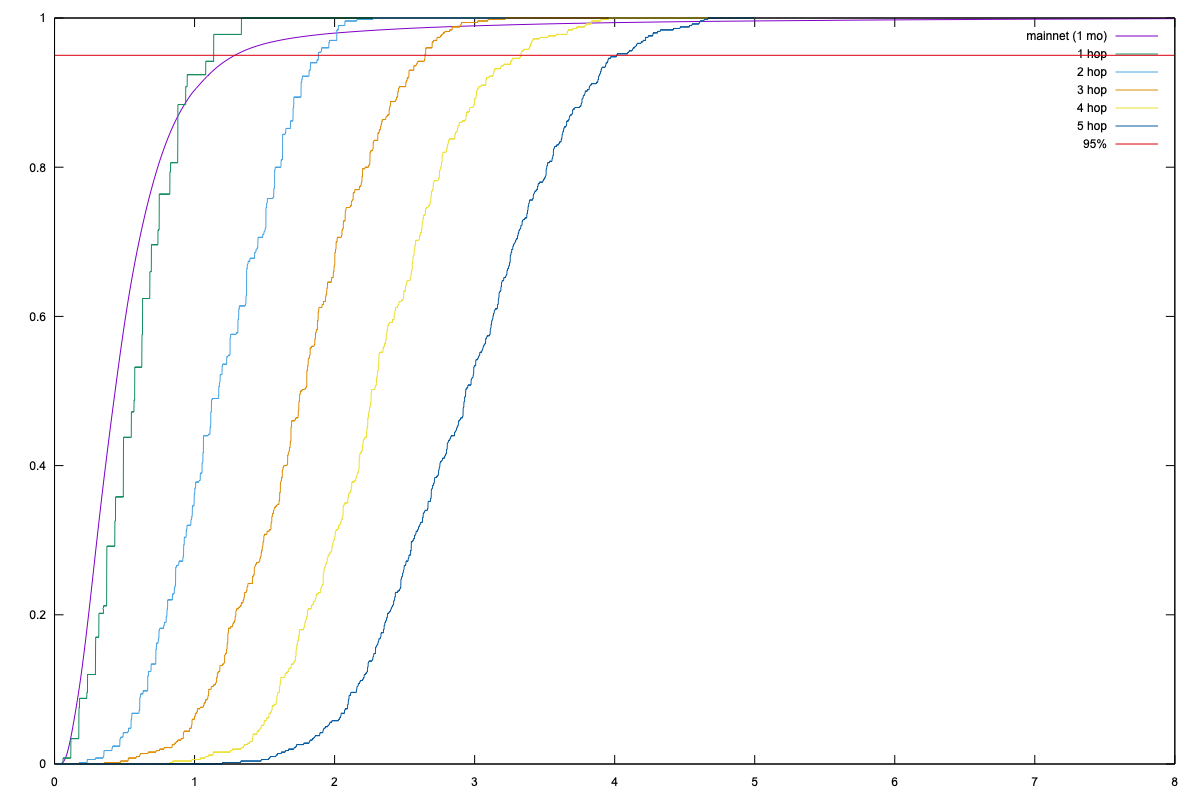
\includegraphics[width=0.68\textwidth]{../diagrams/plot-praos-multi-hops.png}
\caption{Multiple hops \& empirical CDF}
\end{figure}

While this would require some more rigorous analysis to be asserted in a
sound way, it seems there is a good correlation between empirical
distribution and 1-hop distribution, which is comforting as it validates
the relevance of the model.

\subsubsection{Peras ΔQ model -
blocks}\label{peras-ux3b4q-model---blocks}

Things to take into account for modeling Peras:

\begin{itemize}
\tightlist
\item
  \emph{Impact of the size of the certificate:} If adding the
  certificate increases the size of the header beyond the MSS (or MTU?),
  this will impact header diffusion.

  \begin{itemize}
  \tightlist
  \item
    We might need to just add a hash to the header (32 bytes) and then
    have the node request the certificate, which also increases (full)
    header diffusion time.
  \end{itemize}
\item
  \emph{Impact of validating the certificate:} If it is not cheap
  (e.g.~a few ms like a signature verification), this could also lead to
  an increase in block adoption time as a node receiving a header will
  have to add more time to validate it before sharing it with its peers.
\item
  There might not be a certificate for each header, depending on the
  length of the rounds. Given round length \emph{R} in slots and average
  block production length \emph{S}, then frequency of headers with
  certificate is \emph{S}/\emph{R}.

  \begin{itemize}
  \tightlist
  \item
    The model must take into account different paths for retrieving a
    header, one with a certificate and one without.
  \end{itemize}
\item
  Diffusion of votes and certificates does not seem to have other
  impacts on diffusion of blocks: e.g.~just because we have more
  messages to handle and therefore we consume more bandwidth between
  nodes, this could lead to delays for block propagation, but it seems
  there is enough bandwidth (in steady state, perhaps not when syncing)
  to diffuse both votes, certificates, transactions, and blocks without
  one impacting the other.
\end{itemize}

The following diagram compares the ΔQ distribution of block diffusion
(for 4 hops) under different assumptions:

\begin{enumerate}
\def\labelenumi{\arabic{enumi}.}
\tightlist
\item
  Standard block without a certificate,
\item
  Block header points to a certificate.
\end{enumerate}

Certificate validation is assumed to be a constant 50ms.

\begin{figure}
\centering
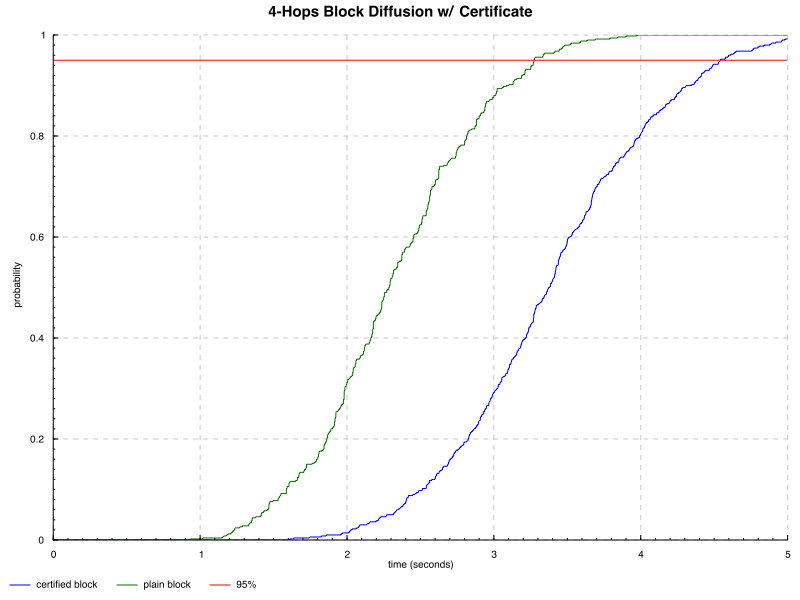
\includegraphics[width=0.68\textwidth]{../diagrams/block-with-cert.png}
\caption{Impact of certificate}
\end{figure}

Obviously, adding a round-trip network exchange to retrieve the
certificate for a given header degrades the ``timeliness'' of block
diffusion. For the case of 2500 nodes with average degree 15, we get the
following distributions, comparing blocks with and without certificates:

\begin{figure}
\centering
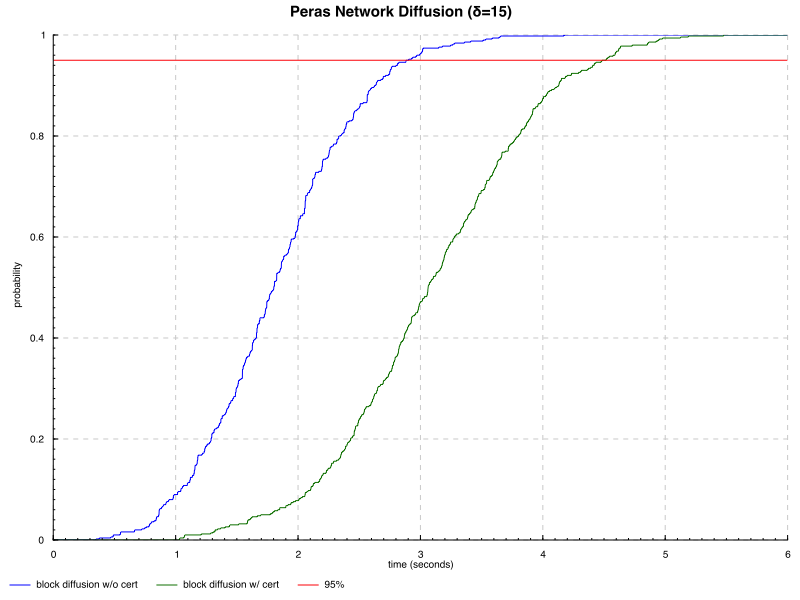
\includegraphics[width=0.68\textwidth]{../diagrams/network-with-cert.png}
\caption{Diffusion with and without certificate}
\end{figure}

\begin{quoting}
 Depending on the value of \(U\), the round length, not all
block headers will have a certificate and the ratio could actually be
quite small, e.g.~if \(T=60\) then we would expect 1/3rd of the headers
to have a certificate on average. While we tried to factor that ratio in
the model, that is misleading because of the second order effect an
additional certificate fetching could have on the whole system: More
delay in the block diffusion process increases the likelihood of forks
which have an adversarial impact on the whole system, and averaging this
impact hides it.
\end{quoting}

\begin{quoting}
 In practice, \texttt{cardano-node} uses \emph{network-level
pipelining} to avoid having to request individually every block/header:
e.g.~when sending multiple blocks to a peer a node will not wait for its
peer's request and will keep sending headers as long as not instructed
to do otherwise.

This is not to be confused with \emph{consensus pipelining} which
streamlines block headers diffusion from upstream to downstream peers
before waiting for full block body validation.
\end{quoting}

\subsubsection{Conclusion}\label{conclusion}

This analysis demonstrates that Peras certificates cannot be on the
critical path of block headers diffusion lest we run the risk of
increased delays in block diffusion and number of forks. Certificates
either have to be small enough to not require an additional round-trip
to transmit on top of the block header, or be part of the block body.
Note that in the latter case the certificates should also be relatively
small as there is limited space available in blocks.

\subsection{Votes \& certificates
diffusion}\label{votes-certificates-diffusion}

Detailed analysis of votes and certificates diffusion is still ongoing
and will be reported in a future document. Some preliminary discussions
with PNSol allowed us to identify the following points to consider:

\begin{itemize}
\tightlist
\item
  The vote diffusion will very likely be unproblematic on ``sunny
  days'', so the modeling and thinking effort should be focused on
  ``rainy days'', e.g.~what happens under heavy load, e.g.~CPU load
  (also possibly network load?). These are the circumstances into which
  backpressure should be applied.
\item
  Some key questions to answer to:

  \begin{itemize}
  \tightlist
  \item
    How much computation do we do on each vote?
  \item
    How much computation do we do on each certificate?
  \item
    What kind of backpressure do we need to bake in?
  \end{itemize}
\item
  An interesting observation: We could build certificates to reduce the
  amount of data transferred, e.g.~trading CPU time (building
  certificate) for space and network bandwidth consumption.
\end{itemize}

\subsection{Impact on user experience}\label{impact-on-user-experience}

\subsubsection{Model}\label{model}

We could want to model the outcomes of Peras in terms of \emph{user
experience}, e.g.~how does Peras impact the user experience? From the
point of view of the users, the thing that matters is the
\emph{settlement time} of their transactions: How long does it take for
a transaction submitted to be \emph{settled}, e.g.~to have enough (how
much?) guarantee that the transaction is definitely part of the chain?

From this point of view, the whole path from transaction submission to
observing a (deep enough) block matters, which means we need to take
into account in our modeling the propagation of the transaction through
the mempools of various nodes in the network until it reaches a block
producer. This also means we need to take into account the potential
\emph{delays} incurred in that journey that can occur because of
\emph{mempool congestion} in the system: When the mempool of a node is
full, it will not pull more transactions from the peers that are
connected to it.

The following diagram illustrates the ``happy path'' of a transaction
until the block its part of gets adopted by the emitting node, in Praos.

\begin{Shaded}
\begin{Highlighting}[]
\NormalTok{sequenceDiagram}
\NormalTok{actor Alice}
\NormalTok{participant N1 as Node1}
\NormalTok{participant N2 as Node2}
\NormalTok{participant N3 as Node3}
\NormalTok{participant BP as Minter}

\NormalTok{N2 {-}{-}\textgreater{}\textgreater{} +N1: Next tx}
\NormalTok{Alice {-}\textgreater{}\textgreater{} N1: Post tx}
\NormalTok{N1 {-}\textgreater{}\textgreater{} +N2: Tx id}
\NormalTok{N2 {-}\textgreater{}\textgreater{} +N1: Get tx}
\NormalTok{N1 {-}\textgreater{}\textgreater{} +N2: Send tx}
\NormalTok{BP {-}{-}\textgreater{}\textgreater{} +N2: Next tx}
\NormalTok{N2 {-}\textgreater{}\textgreater{} +BP: Tx id}
\NormalTok{BP {-}\textgreater{}\textgreater{} +N2: Get tx}
\NormalTok{N2 {-}\textgreater{}\textgreater{} +BP: Send tx}
\NormalTok{BP {-}\textgreater{}\textgreater{} BP: Mint block}
\NormalTok{N2 {-}\textgreater{}\textgreater{} +BP: Next block}
\NormalTok{BP {-}\textgreater{}\textgreater{} N2: Block header}
\NormalTok{N2 {-}\textgreater{}\textgreater{} BP: Get block}
\NormalTok{BP {-}\textgreater{}\textgreater{} N2: Send block}
\NormalTok{N1 {-}\textgreater{}\textgreater{} +N2: Next block}
\NormalTok{N2 {-}\textgreater{}\textgreater{} N1: Block header}
\NormalTok{N1 {-}\textgreater{}\textgreater{} N2: Get block}
\NormalTok{N2 {-}\textgreater{}\textgreater{} N1: Send block}
\NormalTok{N1 {-}{-}\textgreater{}\textgreater{} Alice: Tx in block}
\end{Highlighting}
\end{Shaded}

This question is discussed in much more detail in the
\href{https://docs.google.com/document/d/1B42ep9mvP472-s6p_1qkVmf_b1-McLNPyXGjGHEVJ0w/edit}{report
on timeliness} and should be considered outside of the scope of Peras
protocol itself.

\section{Property-based testing with state-machine based
QuickCheck}\label{property-based-testing-with-state-machine-based-quickcheck}

The \texttt{quickcheck-dynamic} Haskell package enables property-based
testing of state machines. It is the primary testing framework used for
testing the Peras implementations in Haskell and Rust. Eventually, the
dynamic model instances used in \texttt{quickcheck-dynamic} will be
generated directly from the Agda specification of Peras using
\texttt{agda2hs}.

Testing that uses the standard (non-dynamic) \texttt{quickcheck} package
is limited to the JSON serialization tests, such as golden and roundtrip
tests and round-trip tests.

\subsection{Praos properties}\label{praos-properties}

Praos \texttt{NodeModel} and \texttt{NetworkModel} test the state
transitions related to slot leadership and forging blocks. They can be
used with the Haskell node and network implemented in
\texttt{peras-iosim}, or the Rust node and network implementation in
\texttt{peras-rust}. This dual-language capability demonstrated the
feasibility of providing dynamic QuickCheck models for language-agnostic
testing. The properties tested are that the forging rate of a node
matches the theoretical expectation to within statistical variations and
that, sufficiently after genesis, the nodes in a network have a common
chain-prefix.

\subsection{Peras properties}\label{peras-properties}

A \texttt{quickcheck-dynamic} model was created for closer and cleaner
linkage between code generated by \texttt{agda2hs} and Haskell and Rust
simulations. The model has the following features:

The ``idealized'' votes, certificates, blocks, and chains of the
QuickCheck model are separated from ``realized'' ones generated by
\texttt{agda2hs} and used in the simulations. The idealized version
ignores some details like signatures and proofs. It is possible to
remove this separation between ideal and real if behaviors are fully
deterministic (including the bytes of signatures and proofs). However,
this prototype demonstrates the feasibility of having a slightly more
abstract model of a node for use in \texttt{Test.QuickCheck.StateModel}.

The
\href{https://github.com/input-output-hk/peras-design/blob/4bc364f52dd33665cbb13d03d7ca16efea98f4ee/peras-quickcheck/src/Peras/OptimalModel.hs\#L1}{\color{blue}\texttt{\texttt{NodeModel}}}
has sufficient detail to faitfully represents Peras protocol. Ideally,
this would be generated directly by \texttt{agda2hs}. This instance of
\texttt{StateModel} uses the executable specification for state
transitions and includes generators for actions, constrained by
preconditions.

\begin{Shaded}
\begin{Highlighting}[]
\KeywordTok{data} \DataTypeTok{NodeModel} \OtherTok{=} \DataTypeTok{NodeModel}\NormalTok{ \{ }\OperatorTok{...}\NormalTok{ \}}
\end{Highlighting}
\end{Shaded}

\begin{Shaded}
\begin{Highlighting}[]
\KeywordTok{instance} \DataTypeTok{StateModel} \DataTypeTok{NodeModel} \KeywordTok{where}
  \KeywordTok{data} \DataTypeTok{Action} \DataTypeTok{NodeModel}\NormalTok{ a }\KeywordTok{where}
    \DataTypeTok{Initialize}\OtherTok{ ::} \DataTypeTok{Protocol} \OtherTok{{-}\textgreater{}} \DataTypeTok{PartyId} \CommentTok{\{{-} i.e., the owner of the node {-}\}} \OtherTok{{-}\textgreater{}} \DataTypeTok{Action} \DataTypeTok{NodeModel}\NormalTok{ ()}
    \DataTypeTok{ATick}\OtherTok{ ::} \DataTypeTok{IsSlotLeader} \OtherTok{{-}\textgreater{}} \DataTypeTok{IsCommitteeMember} \OtherTok{{-}\textgreater{}} \DataTypeTok{Action} \DataTypeTok{NodeModel}\NormalTok{ [}\DataTypeTok{MessageIdeal}\NormalTok{]}
    \DataTypeTok{ANewChain}\OtherTok{ ::} \DataTypeTok{ChainIdeal} \OtherTok{{-}\textgreater{}} \DataTypeTok{Action} \DataTypeTok{NodeModel}\NormalTok{ [}\DataTypeTok{MessageIdeal}\NormalTok{]}
    \DataTypeTok{ASomeCert}\OtherTok{ ::} \DataTypeTok{CertIdeal} \OtherTok{{-}\textgreater{}} \DataTypeTok{Action} \DataTypeTok{NodeModel}\NormalTok{ [}\DataTypeTok{MessageIdeal}\NormalTok{]}
    \DataTypeTok{ASomeVote}\OtherTok{ ::} \DataTypeTok{VoteIdeal} \OtherTok{{-}\textgreater{}} \DataTypeTok{Action} \DataTypeTok{NodeModel}\NormalTok{ [}\DataTypeTok{MessageIdeal}\NormalTok{]}
\NormalTok{  arbitraryAction }\OtherTok{=} \OperatorTok{...}
\NormalTok{  precondition }\OtherTok{=} \OperatorTok{...}
\NormalTok{  initialState }\OtherTok{=} \OperatorTok{...}
\NormalTok{  nextState }\OtherTok{=} \OperatorTok{...}
\end{Highlighting}
\end{Shaded}

The executable specification for the node model is embodied in a
typeclass \texttt{PerasNode} representing the abstract interface of
nodes. An
\texttt{instance\ (Monad\ m,\ PerasNode\ n\ m)\ =\textgreater{}\ RunModel\ NodeModel\ (RunMonad\ n\ m)}
executes actions on a \texttt{PerasNode} and checks postconditions. This
also could be generated by \texttt{agda2hs} from the specification.

\begin{Shaded}
\begin{Highlighting}[]
\KeywordTok{class} \DataTypeTok{Monad}\NormalTok{ m }\OtherTok{=\textgreater{}} \DataTypeTok{PerasNode}\NormalTok{ a m }\KeywordTok{where}
\OtherTok{  newSlot ::} \DataTypeTok{IsSlotLeader} \OtherTok{{-}\textgreater{}} \DataTypeTok{IsCommitteeMember} \OtherTok{{-}\textgreater{}}\NormalTok{ a }\OtherTok{{-}\textgreater{}}\NormalTok{ m ([}\DataTypeTok{Message}\NormalTok{], a)}
\OtherTok{  newChain ::} \DataTypeTok{Chain} \OtherTok{{-}\textgreater{}}\NormalTok{ a }\OtherTok{{-}\textgreater{}}\NormalTok{ m ([}\DataTypeTok{Message}\NormalTok{], a)}
  \OperatorTok{...}
\end{Highlighting}
\end{Shaded}

For demonstration purposes, an \texttt{instance\ PerasNode\ ExampleNode}
implements a simple, intentionally buggy, node for exercising the
dynamic logic tests. This could be a full Haskell or Rust
implementation, an implementation generated via \texttt{agda2hs} from
operational (executable) semantics in Agda, etc.

\begin{Shaded}
\begin{Highlighting}[]
\KeywordTok{data} \DataTypeTok{ExampleNode} \OtherTok{=} \DataTypeTok{ExampleNode}\NormalTok{ \{ }\OperatorTok{...}\NormalTok{ \}}

\KeywordTok{instance} \DataTypeTok{PerasNode} \DataTypeTok{ExampleNode} \DataTypeTok{Gen} \KeywordTok{where}
  \OperatorTok{...}
\end{Highlighting}
\end{Shaded}

The example property below simply runs a simulation using
\texttt{ExampleNode} and checks the trace conforms to the executable
specification.

\begin{Shaded}
\begin{Highlighting}[]
\OtherTok{propSimulate ::}\NormalTok{ (}\DataTypeTok{Actions} \DataTypeTok{NodeModel} \OtherTok{{-}\textgreater{}} \DataTypeTok{Property}\NormalTok{) }\OtherTok{{-}\textgreater{}} \DataTypeTok{Property}
\NormalTok{propSimulate }\OtherTok{=}\NormalTok{ forAllDL simulate}

\OtherTok{simulate ::} \DataTypeTok{DL} \DataTypeTok{NodeModel}\NormalTok{ ()}
\NormalTok{simulate }\OtherTok{=}\NormalTok{ action initialize }\OperatorTok{\textgreater{}\textgreater{}}\NormalTok{ anyActions\_}

\CommentTok{{-}{-} | Act on the example node.}
\OtherTok{propOptimalModelExample ::} \DataTypeTok{Actions} \DataTypeTok{NodeModel} \OtherTok{{-}\textgreater{}} \DataTypeTok{Property}
\NormalTok{propOptimalModelExample actions }\OtherTok{=}\NormalTok{ property }\OperatorTok{.}\NormalTok{ runPropExampleNode }\OperatorTok{$} \KeywordTok{do}
\NormalTok{  void }\OperatorTok{$}\NormalTok{ runActions actions}
\NormalTok{  assert }\DataTypeTok{True}

\CommentTok{{-}{-} | Test a property in the example node.}
\OtherTok{runPropExampleNode ::} \DataTypeTok{Testable}\NormalTok{ a }\OtherTok{=\textgreater{}} \DataTypeTok{PropertyM}\NormalTok{ (}\DataTypeTok{RunMonad} \DataTypeTok{ExampleNode} \DataTypeTok{Gen}\NormalTok{) a }\OtherTok{{-}\textgreater{}} \DataTypeTok{Gen} \DataTypeTok{Property}
\NormalTok{runPropExampleNode p }\OtherTok{=} \KeywordTok{do}
  \DataTypeTok{Capture}\NormalTok{ eval }\OtherTok{\textless{}{-}}\NormalTok{ capture}
  \FunctionTok{flip}\NormalTok{ evalStateT def }\OperatorTok{.}\NormalTok{ runMonad }\OperatorTok{.}\NormalTok{ eval }\OperatorTok{$}\NormalTok{ monadic\textquotesingle{} p}
\end{Highlighting}
\end{Shaded}

Because the example node contains a couple of intentional bugs, one
expects the test to fail. Shrinking reveals a parsimonious series of
actions that exhibit one of the bugs.

\begin{Shaded}
\begin{Highlighting}[]
\OtherTok{spec ::} \DataTypeTok{Spec}
\NormalTok{spec }\OtherTok{=}\NormalTok{ describe }\StringTok{"Example node"} \OperatorTok{.}\NormalTok{ prop }\StringTok{"Simulation respects model"}
         \OperatorTok{.}\NormalTok{ expectFailure }\OperatorTok{$}\NormalTok{ propSimulate propOptimalModelExample}
\end{Highlighting}
\end{Shaded}

\begin{Shaded}
\begin{Highlighting}[]
\NormalTok{$ cabal run test:peras{-}quickcheck{-}test {-}{-} {-}{-}match "/Peras.OptimalModel/Example node/Simulation respects model/"}

\NormalTok{Peras.OptimalModel}
\NormalTok{  Example node}
\NormalTok{    Simulation respects model [✔]}
\NormalTok{      +++ OK, failed as expected. Assertion failed (after 4 tests and 1 shrink):}
\NormalTok{      do action $ Initialize (Peras \{roundLength = 10, quorum = 3, boost = 0.25\}) 0}
\NormalTok{         action $ ANewChain [BlockIdeal \{hash = "92dc9c1906312bb4", creator = 1, slot = 0, cert = Nothing, parent = ""\}]}
\NormalTok{         action $ ATick False True}
\NormalTok{         pure ()}

\NormalTok{Finished in 0.0027 seconds}
\NormalTok{1 example, 0 failures}
\end{Highlighting}
\end{Shaded}

\subsection{Relating test model to formal
model}\label{relating-test-model-to-formal-model}

The team has been working with
\href{https://drive.google.com/file/d/1vDfwiR24t3K6INkabwR43A4Ryc-j7SzG/view}{\color{blue}\texttt{\emph{Quviq}}}
to provide assistance and expertise on tighter integration between the
Agda specification and the \texttt{quickcheck-dynamic} model. This work
resulted in the development of a prototype that demonstrates the
feasibility of generating the \texttt{quickcheck-dynamic} model from the
Agda specification, as described in Milestone 1 of the \emph{Statement
of Work}.

The following picture summarizes how the various parts of the testing
framework for Peras are related:

\begin{figure}
\centering
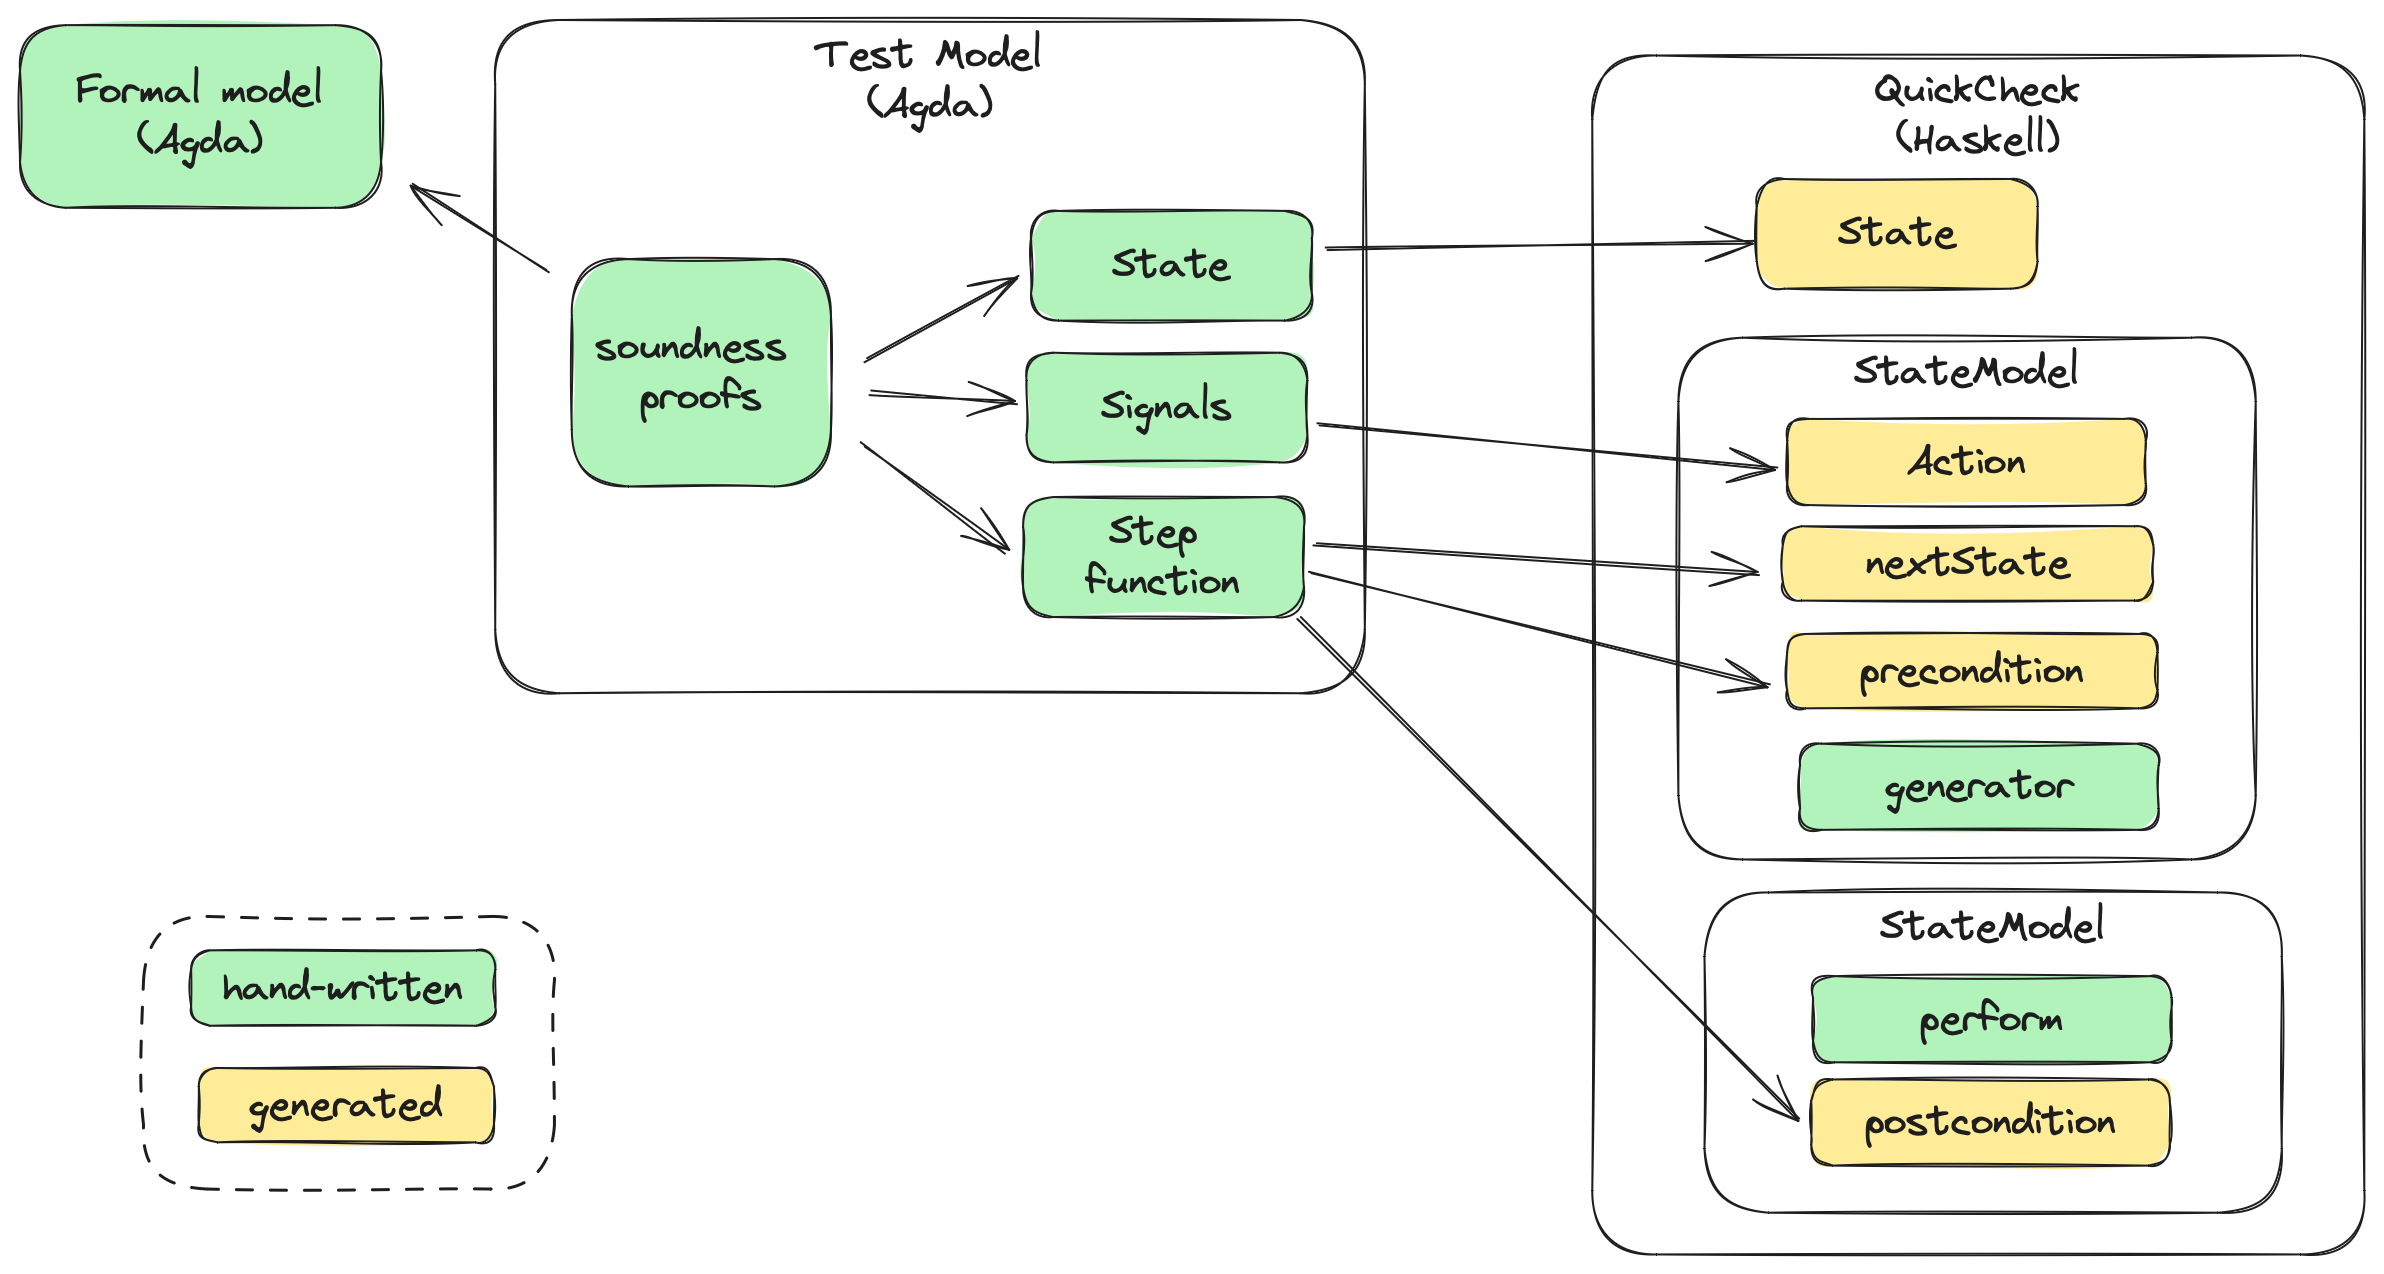
\includegraphics{../diagrams/agda-quickcheck.png}
\caption{Agda-QuickCheck Integration}
\end{figure}

The key points of this line of work are:

\begin{enumerate}
\def\labelenumi{\arabic{enumi}.}
\tightlist
\item
  While both written in Agda, we differentiate the \emph{Formal model}
  from the \emph{Test model} as they serve different purposes. More
  importantly, we acknowledge the fact there be more than one \emph{Test
  model} for a given \emph{Formal model}, depending on the level of
  abstraction and the properties we want to test,
\item
  The \emph{Formal model} is the actual
  \hyperref[agda-specification]{specification} of the protocol and is
  meant to write \emph{proofs} related to the protocol (e.g the usual
  blockchain properties like chain growth, chain quality, etc. and the
  specific properties of Peras). Ideally, this model should be part of
  the research work and written in close collaboration with them,
\item
  The \emph{Test model} describes some relevant behavior of the system
  for the purpose of asserting a liveness or safety property, in the
  form of a state machine relating: A state data type, some
  \emph{signals} sent to the SUT for testing purpose, and a \emph{step}
  function describing possible transitions of the system,
\item
  The \emph{Test model}'s soundness w.r.t the \emph{Formal model} is
  proven through a \emph{soundness} theorem that guarantees each
  sequence of transition in the \emph{Test model} can be mapped to a
  valid sequence of transitions in the \emph{Formal model},
\item
  Using \texttt{agda2hs} Haskell code is generated from the \emph{Test
  model} and integrated in a small hand-written wrapper complying with
  quickcheck-dynamic API,
\item
  Note the \texttt{perform} function is not generated because it's
  specific to the actual implementation of the \emph{System-Under-Test}
  (SUT).
\end{enumerate}

The provided models are very simple toy examples of some chain protocol
as the purpose of this first step was to validate the approach and
identify potential issues. In further steps, we need to:

\begin{enumerate}
\def\labelenumi{\arabic{enumi}.}
\tightlist
\item
  Work on a more complex and realistic Test model checking some core
  properties of the Peras protocol,
\item
  Ensure the Formal model's semantics is amenable to testability and
  proving soundness of the Test model.
\end{enumerate}

\section{Simulations}\label{simulations}

In order to test the language-neutrality of the testing framework for
Peras, we developed both Haskell-based and Rust-based simulations of the
Peras and Praos protocols.

\subsection{Haskell-based simulation}\label{haskell-based-simulation}

The initial phase of the first Peras PI's work on simulation revolves
around discovery. This involves several key tasks, including prototyping
and evaluating different simulation architectures, investigating
simulation-based analysis workflows, assessing existing network
simulation tools, establishing interface and serialization formats,
eliciting requirements for both simulation and analysis purposes, and
gaining a deeper understanding of Peras behaviors. The first prototype
simulation, developed in Haskell, is closely intertwined with the Agda
specification. This integration extends to the generation of types
directly from Agda. Subsequent work will migrate a significant portion
of the Peras implementation from Haskell to functions within the Agda
specification, which will necessitate reconceptualizing and refining
various components of the simulation.

The Peras simulation employs language-agnostic components that
collaborate seamlessly (see figure below). This includes node
implementations in Haskell, with Rust implementations forthcoming.
Additionally, the native-Haskell simulation utilizes the
\href{https://hackage.haskell.org/package/io-classes}{\color{blue}\texttt{IOSim}} packages in
a manner consistent with QuickCheck tests in \texttt{peras-quickcheck},
which also supports a \emph{Foreign Function Interface} (FFI) connection
to \href{https://github.com/input-output-hk/ce-netsim}{\color{blue}\texttt{Netsim}} and
\texttt{peras-rust}. The simulation setup also encompasses statistically
designed experiments, the ability to inject rare events or adversarial
behaviors, tools for generating networks and scenarios, as well as
analysis and visualization tools to interpret the simulation results. A
significant aspect of the workflow is geared towards analysis. This
involves an observability approach to gathering metrics, utilization of
language-independent file formats, visualization of network structures,
and statistical analyses primarily conducted using
\href{https://www.r-project.org/}{\color{blue}\texttt{R}}.

\begin{figure}
\centering
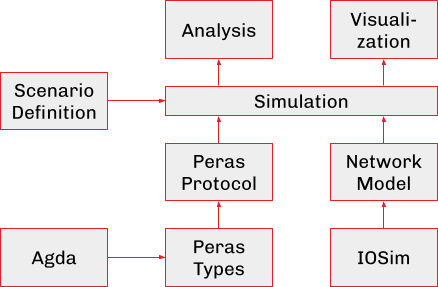
\includegraphics[width=0.48\textwidth]{../diagrams/sim-expts/sim-workflow.png}
\caption{Workflow for simulation experiments}
\end{figure}

The IOSim-based Haskell simulator for Peras currently provides a
provisional implementation of the Peras protocol's intricacies,
including committee selection, voting rounds, and cool-down periods.
Presently, the fidelity of the simulation to the Peras protocol is
moderate, while the fidelity at the network layer remains low.
Substantial refactoring and refinement efforts are deemed necessary
moving forward to enhance the simulation's accuracy and effectiveness.

The simulation implements the February version of the Peras protocol,
illustrated in the
\href{https://en.wikipedia.org/wiki/Unified_Modeling_Language}{\color{blue}\texttt{UML}}
sequence diagrams below for node behavior, and the activity diagram for
node state transitions. Nodes receive messages for entering a new slot
or new voting round; they also receive new preferred chains or votes
from their upstream peers via messages. When they vote, forge blocks, or
adopt a new preferred chain, they notify their downstream peers via
messages.

\begin{quoting}
The detailed behavior of the February protocol differs
somewhat from later versions such as the March protocol.
\end{quoting}

\begin{figure}
\centering
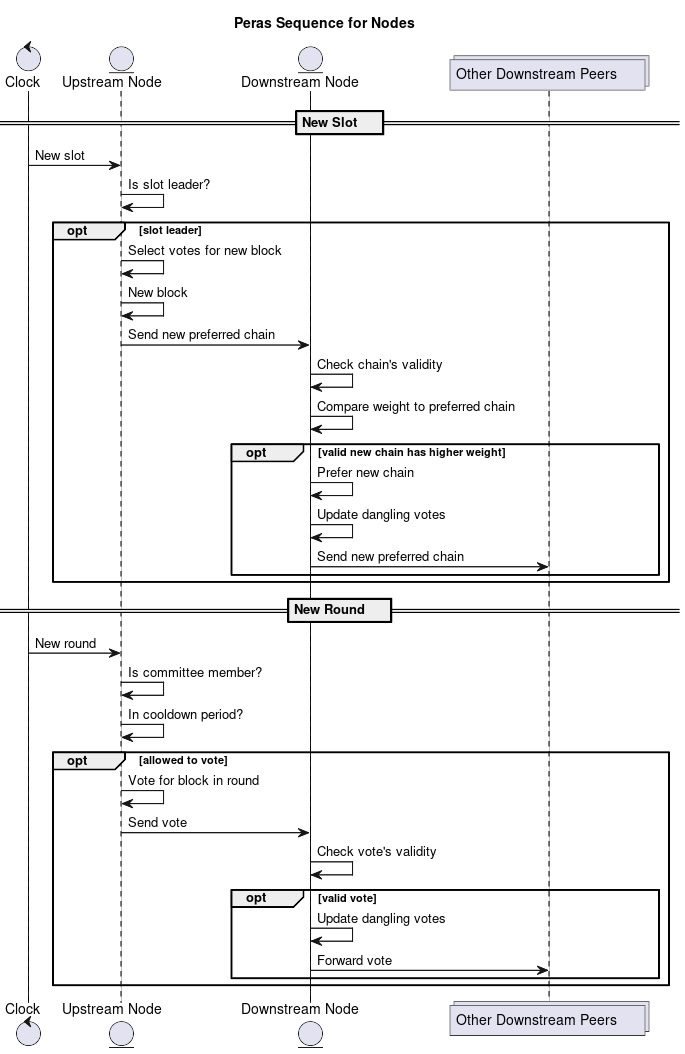
\includegraphics[width=0.68\textwidth]{../diagrams/sim-expts/peras-sequence.jpg}
\caption{UML sequence diagram for the February version of the Peras
protocol}
\end{figure}

\begin{figure}
\centering
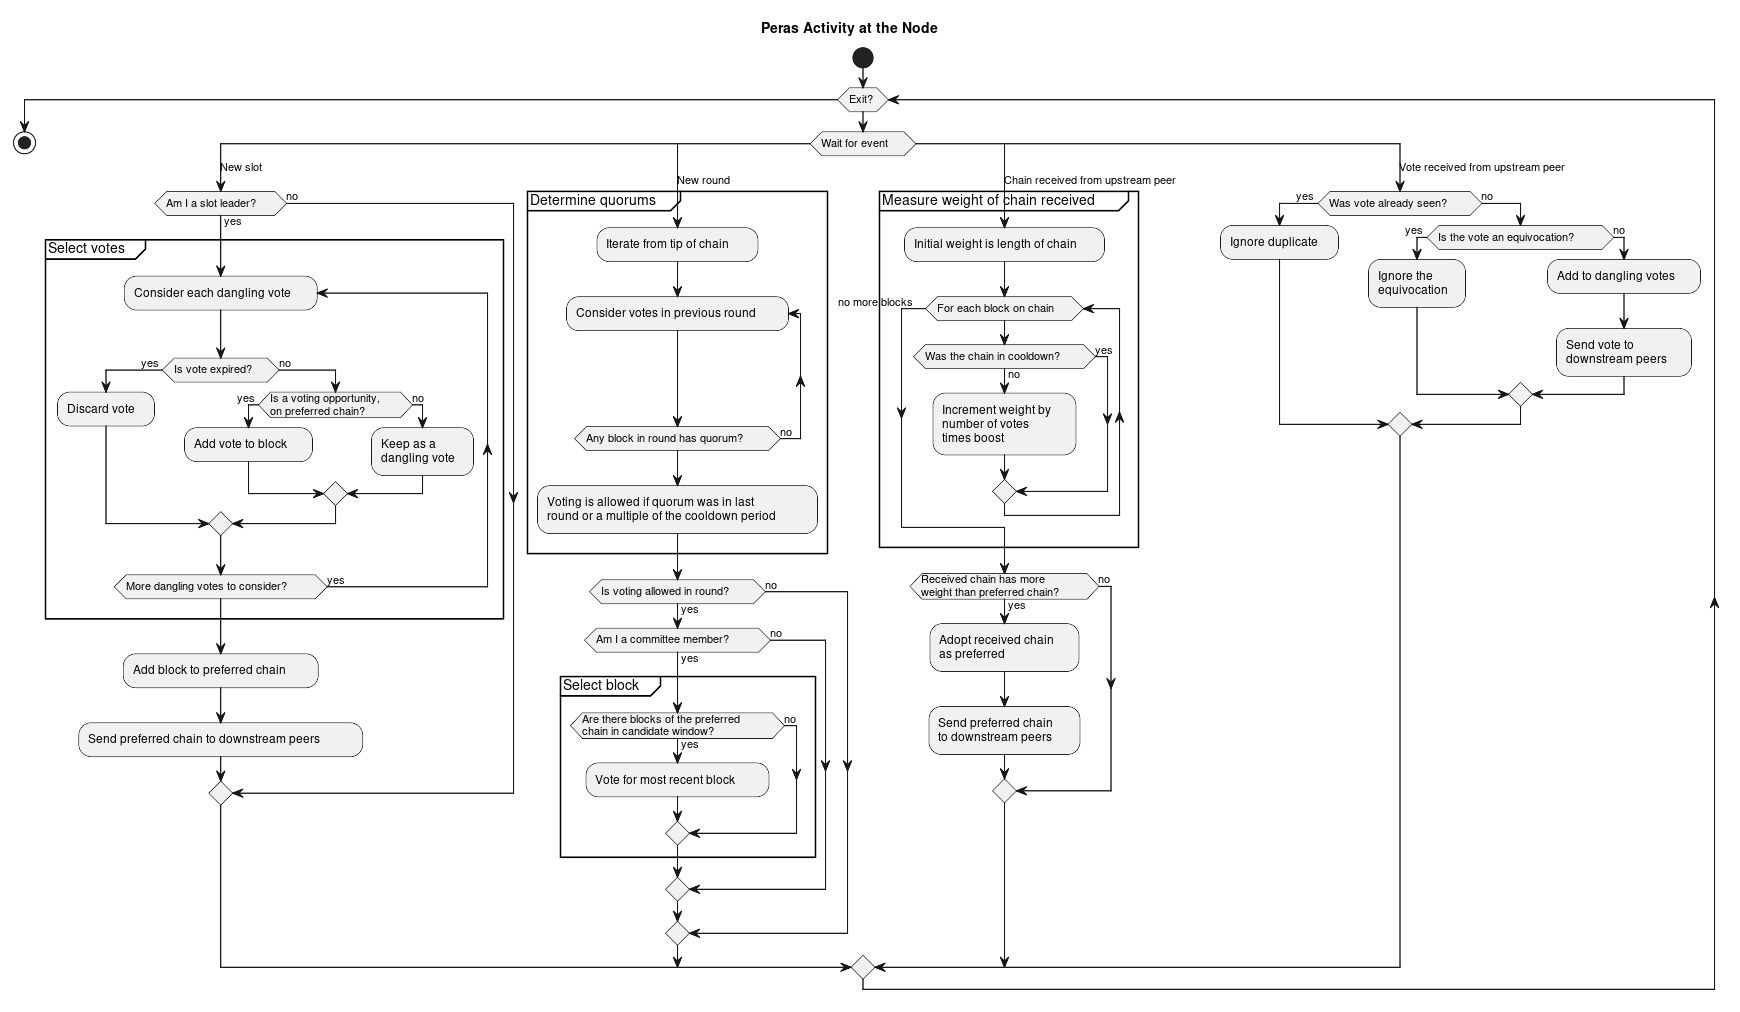
\includegraphics[width=0.80\textwidth]{../diagrams/sim-expts/peras-activity.jpg}
\caption{UML activity diagram for the February version of the Peras
protocol}
\end{figure}

\subsubsection{Design}\label{design}

The architecture, design, and implementation of the Haskell-based
\texttt{peras-iosim} package evolved significantly during Peras's first
PI, so here we just summarize the software approach that the series of
prototypes has converged upon.

\paragraph{IOSim}\label{iosim}

The simulator initially relied heavily on \texttt{io-sim} and
\texttt{io-classes} as it was inspired by similar work based on IOSim,
like \href{https://github.com/input-output-hk/hydra-sim}{\color{blue}\texttt{hydra-sim}}:
Each node would be a separate actor, possibly running several threads.
We then moved to a much more lightweight use of IOSim's capabilities.

First of all, IOSim's implementation is currently single-threaded with a
centralized scheduler that handles the simulated threads. Thus, IOSim
does not provide the speed advantages of a parallel simulator. However,
it conveniently provides many of the commonly used MTL (monad
transformer library) instances typically used with \texttt{IO} or
\texttt{MonadIO} but in a manner compatible with a simulation
environment. For example, \texttt{threadDelay} in \texttt{IOSim}
simulates the passage of time whereas in \texttt{IO} it blocks while
time actually passes. Furthermore, the STM usage in earlier Peras
prototypes was first refactored to higher-level constructs (such as STM
in the network simulation layer instead of in the nodes themselves) but
then finally eliminated altogether. The elimination of STM reduces the
boilerplate and thread orchestration in QuickCheck tests and provides a
cleaner testing interface to the node, so that interface is far less
language dependent. Overall, the added complexity of STM simply was not
justified by requirements for the node, since the reference node
purposefully should not be highly optimized. Additionally, IOSim's event
logging is primarily used to handle logging via the
\texttt{contra-tracer} package. IOSim's \texttt{MonadTime} and
\texttt{MonadTimer} classes are used for managing the simulation of the
passage of time.

\paragraph{Node interface}\label{node-interface}

The node interface has evolved towards a request-response pattern, with
several auxiliary getters and setters. This will further evolve as
alignment with the Agda-generated code and QuickCheck Dynamic become
tighter. At this point, however, the node interface and implementation
is sufficient for a fully faithful simulation of the protocol, along
with the detailed observability required for quantifying and debugging
its performance.

\begin{Shaded}
\begin{Highlighting}[]
\KeywordTok{class} \DataTypeTok{PerasNode}\NormalTok{ a }\KeywordTok{where}
\OtherTok{  getNodeId ::}\NormalTok{ a }\OtherTok{{-}\textgreater{}} \DataTypeTok{NodeId}
\OtherTok{  getOwner ::}\NormalTok{ a }\OtherTok{{-}\textgreater{}} \DataTypeTok{PartyId}
\OtherTok{  getStake ::}\NormalTok{ a }\OtherTok{{-}\textgreater{}} \DataTypeTok{Coin}
\OtherTok{  setStake ::}\NormalTok{ a }\OtherTok{{-}\textgreater{}} \DataTypeTok{Coin} \OtherTok{{-}\textgreater{}}\NormalTok{ a}
\OtherTok{  getDownstreams ::}\NormalTok{ a }\OtherTok{{-}\textgreater{}}\NormalTok{ [}\DataTypeTok{NodeId}\NormalTok{]}
\OtherTok{  getPreferredChain ::}\NormalTok{ a }\OtherTok{{-}\textgreater{}} \DataTypeTok{Chain}
\OtherTok{  getPreferredVotes ::}\NormalTok{ a }\OtherTok{{-}\textgreater{}}\NormalTok{ [}\DataTypeTok{Vote}\NormalTok{]}
\OtherTok{  getPreferredCerts ::}\NormalTok{ a }\OtherTok{{-}\textgreater{}}\NormalTok{ [}\DataTypeTok{Certificate}\NormalTok{]}
\OtherTok{  getPreferredBodies ::}\NormalTok{ a }\OtherTok{{-}\textgreater{}}\NormalTok{ [}\DataTypeTok{BlockBody}\NormalTok{]}
\OtherTok{  handleMessage ::} \DataTypeTok{Monad}\NormalTok{ m }\OtherTok{=\textgreater{}}\NormalTok{ a }\OtherTok{{-}\textgreater{}} \DataTypeTok{NodeContext}\NormalTok{ m }\OtherTok{{-}\textgreater{}} \DataTypeTok{InEnvelope} \OtherTok{{-}\textgreater{}}\NormalTok{ m (}\DataTypeTok{NodeResult}\NormalTok{, a)}
\OtherTok{  stop ::} \DataTypeTok{Monad}\NormalTok{ m }\OtherTok{=\textgreater{}}\NormalTok{ a }\OtherTok{{-}\textgreater{}} \DataTypeTok{NodeContext}\NormalTok{ m }\OtherTok{{-}\textgreater{}}\NormalTok{ m a}
\end{Highlighting}
\end{Shaded}

Honest versus adversarial nodes can be wrapped in the existential type
\texttt{SomeNode}. The \texttt{NodeResult} captures the messages emitted
by the node in response to the message (\texttt{InEnvelope}) that it
receives, specifies the lower bound on the time of the node's next
activity (\texttt{wakeup}), and collects metrics regarding the node's
activity:

\begin{Shaded}
\begin{Highlighting}[]
\KeywordTok{data} \DataTypeTok{NodeResult} \OtherTok{=} \DataTypeTok{NodeResult}
\NormalTok{  \{}\OtherTok{ wakeup ::} \DataTypeTok{UTCTime}
\NormalTok{  ,}\OtherTok{ outputs ::}\NormalTok{ [}\DataTypeTok{OutEnvelope}\NormalTok{]}
\NormalTok{  ,}\OtherTok{ stats ::} \DataTypeTok{NodeStats}
\NormalTok{  \}}

\KeywordTok{data} \DataTypeTok{NodeStats} \OtherTok{=} \DataTypeTok{NodeStats}
\NormalTok{  \{}\OtherTok{ preferredTip ::}\NormalTok{ [(}\DataTypeTok{Slot}\NormalTok{, }\DataTypeTok{BlockHash}\NormalTok{)]}
\NormalTok{  ,}\OtherTok{ rollbacks ::}\NormalTok{ [}\DataTypeTok{Rollback}\NormalTok{]}
\NormalTok{  , }\OperatorTok{...}
\NormalTok{  \}}
\end{Highlighting}
\end{Shaded}

The \texttt{NodeContext} includes critical environmental information
such as the current time and the total stake in the system:

\begin{Shaded}
\begin{Highlighting}[]
\KeywordTok{data} \DataTypeTok{NodeContext}\NormalTok{ m }\OtherTok{=} \DataTypeTok{NodeContext}
\NormalTok{  \{}\OtherTok{ protocol ::} \DataTypeTok{Protocol}
\NormalTok{  ,}\OtherTok{ totalStake ::} \DataTypeTok{Coin}
\NormalTok{  ,}\OtherTok{ slot ::} \DataTypeTok{Slot}
\NormalTok{  ,}\OtherTok{ clock ::} \DataTypeTok{UTCTime}
\NormalTok{  ,}\OtherTok{ traceSelf ::} \DataTypeTok{TraceSelf}\NormalTok{ m}
\NormalTok{  \}}
\end{Highlighting}
\end{Shaded}

\paragraph{Auxiliary data structures}\label{auxiliary-data-structures}

An efficient Haskell simulation requires auxiliary data structures to
index the blocks, votes, and certificates in the block tree, to memoize
quorum checks, etc. A node can use a small state machine for each
channel to an upstream node and supplement that with its own global
state machine.

\begin{Shaded}
\begin{Highlighting}[]
\KeywordTok{data} \DataTypeTok{ChainState} \OtherTok{=} \DataTypeTok{ChainState}
\NormalTok{  \{}\OtherTok{ tracker ::} \DataTypeTok{ChainTracker}
\NormalTok{  ,}\OtherTok{ channelTrackers ::} \DataTypeTok{Map} \DataTypeTok{NodeId} \DataTypeTok{ChainTracker}
\NormalTok{  ,}\OtherTok{ chainIndex ::} \DataTypeTok{ChainIndex}
\NormalTok{  \}}
\end{Highlighting}
\end{Shaded}

Each \texttt{ChainTracker} records node- or peer-specific states.

\begin{Shaded}
\begin{Highlighting}[]
\KeywordTok{data} \DataTypeTok{ChainTracker} \OtherTok{=} \DataTypeTok{ChainTracker}
\NormalTok{  \{}\OtherTok{ preferredChain ::} \DataTypeTok{Chain}
\NormalTok{  ,}\OtherTok{ preferredVoteHashes ::} \DataTypeTok{Set} \DataTypeTok{VoteHash}
\NormalTok{  ,}\OtherTok{ preferredCertHashes ::} \DataTypeTok{Set} \DataTypeTok{CertificateHash}
\NormalTok{  ,}\OtherTok{ missingBodies ::} \DataTypeTok{Set} \DataTypeTok{BodyHash}
\NormalTok{  ,}\OtherTok{ latestSeen ::} \DataTypeTok{Maybe} \DataTypeTok{Certificate}
\NormalTok{  ,}\OtherTok{ latestPreferred ::} \DataTypeTok{Maybe} \DataTypeTok{Certificate}
\NormalTok{  \}}
\end{Highlighting}
\end{Shaded}

An index facilitates efficient lookup and avoids recomputation of quorum
information.

\begin{Shaded}
\begin{Highlighting}[]
\KeywordTok{data} \DataTypeTok{ChainIndex} \OtherTok{=} \DataTypeTok{ChainIndex}
\NormalTok{  \{}\OtherTok{ headerIndex ::} \DataTypeTok{Map} \DataTypeTok{BlockHash} \DataTypeTok{Block}
\NormalTok{  ,}\OtherTok{ bodyIndex ::} \DataTypeTok{Map} \DataTypeTok{BodyHash} \DataTypeTok{BlockBody}
\NormalTok{  ,}\OtherTok{ voteIndex ::} \DataTypeTok{Map} \DataTypeTok{VoteHash} \DataTypeTok{Vote}
\NormalTok{  ,}\OtherTok{ certIndex ::} \DataTypeTok{Map} \DataTypeTok{CertificateHash} \DataTypeTok{Certificate}
\NormalTok{  ,}\OtherTok{ votesByRound ::} \DataTypeTok{Map} \DataTypeTok{RoundNumber}\NormalTok{ (}\DataTypeTok{Set} \DataTypeTok{VoteHash}\NormalTok{)}
\NormalTok{  ,}\OtherTok{ certsByRound ::} \DataTypeTok{Map} \DataTypeTok{RoundNumber}\NormalTok{ (}\DataTypeTok{Set} \DataTypeTok{VoteHash}\NormalTok{)}
\NormalTok{  ,}\OtherTok{ weightIndex ::} \DataTypeTok{Map} \DataTypeTok{BlockHash} \DataTypeTok{Double}
\NormalTok{  \}}
\end{Highlighting}
\end{Shaded}

Combined, these types allow a node to track the information it has sent
or received from downstream or upstream peers, to eliminate recomputing
chain weights, to avoid asking multiple peers for the same information,
and to record its and its peers' preferred chains, votes, and
certificates. Note that this instrumentation and optimization does not
affect the simulated performance of the node because that performance is
tracked via a cost model, regardless of the performance of the
simulation code.

\paragraph{Observability}\label{observability}

Tracing occurs via a \texttt{TraceReport} which records ad-hoc
information or the structured statistics.

\begin{Shaded}
\begin{Highlighting}[]
\KeywordTok{data} \DataTypeTok{TraceReport}
  \OtherTok{=} \DataTypeTok{TraceValue}
\NormalTok{      \{}\OtherTok{ self ::} \DataTypeTok{NodeId}
\NormalTok{      ,}\OtherTok{ slot ::} \DataTypeTok{Slot}
\NormalTok{      ,}\OtherTok{ clock ::} \DataTypeTok{UTCTime}
\NormalTok{      ,}\OtherTok{ value ::} \DataTypeTok{Value}
\NormalTok{      \}}
  \OperatorTok{|} \DataTypeTok{TraceStats}
\NormalTok{      \{}\OtherTok{ self ::} \DataTypeTok{NodeId}
\NormalTok{      ,}\OtherTok{ slot ::} \DataTypeTok{Slot}
\NormalTok{      ,}\OtherTok{ clock ::} \DataTypeTok{UTCTime}
\NormalTok{      ,}\OtherTok{ statistics ::} \DataTypeTok{NodeStats}
\NormalTok{      \}}
\end{Highlighting}
\end{Shaded}

The \texttt{value} in the interface above can hold the result of a
single ``big step'', recorded in a \texttt{StepResult} of outputs and
events.

\begin{Shaded}
\begin{Highlighting}[]
\KeywordTok{data} \DataTypeTok{StepResult} \OtherTok{=} \DataTypeTok{StepResult}
\NormalTok{  \{}\OtherTok{ stepTime ::} \DataTypeTok{UTCTime}
\NormalTok{  ,}\OtherTok{ stepOutputs ::}\NormalTok{ [}\DataTypeTok{OutEnvelope}\NormalTok{]}
\NormalTok{  ,}\OtherTok{ stepEvents ::}\NormalTok{ [}\DataTypeTok{Event}\NormalTok{]}
\NormalTok{  \}}

\KeywordTok{data} \DataTypeTok{Event}
  \OtherTok{=} \DataTypeTok{Send}\NormalTok{ \{ }\OperatorTok{...}\NormalTok{ \}}
  \OperatorTok{|} \DataTypeTok{Drop}\NormalTok{ \{ }\OperatorTok{...}\NormalTok{ \}}
  \OperatorTok{|} \OperatorTok{...}
  \OperatorTok{|} \DataTypeTok{Trace} \DataTypeTok{Value}
\end{Highlighting}
\end{Shaded}

The \texttt{peras-iosim} executable supports optional capture of the
trace as a stream of JSON objects. In experiments, \texttt{jq} is used
for ad-hoc data extraction and \texttt{mongo} is used for complex
queries. The result is analyzed using R scripts.

\paragraph{Message routing}\label{message-routing}

The messaging and state-transition behavior of the network of nodes can
be modeled via a discrete event simulation (DES). Such simulations are
often parallelized (PDES) in order to take advantage of the speed gains
possible from multiple threads of execution. Otherwise, a single thread
must manage routing of messages and nodes' computations: for large
networks and long simulated times, the simulation's execution may become
prohibitively slow. Peras simulations are well suited to
\emph{conservative PDES} where strong guarantees ensure that messages
are always delivered at monotonically non-decreasing times to each node;
the alternative is an \emph{optimistic PDES} where the node and/or
message queue states have to be rolled back if a message with an
out-of-order timestamp is delivered. A PDES for Peras can be readily
constructed if each time a node emits a message it also declares a
guarantee that it will not emit another message until a specified later
time. Such declarations provide sufficient information for its
downstream peers to advance their clocks to the minimum timestamp
guaranteed by their upstream peers: i.e., when a node sees empty
incoming message queues from all of its upstream peers, it can compute a
safe time to advance forward, thus avoiding race conditions or deadlock.
Hence, each node can run its own thread and have upstream and downstream
message queues directly connected to its peers, all without the
centrally managed message routing that would form a potential bottleneck
for scaling performance. The experiments described later in this
document indicate that PDES is not needed at this time because
simulations execute sufficiently fast without it and the cpu resources
could be better used for running ensembles of simulations in parallel.

That said, it likely is the case that Peras simulations will not need to
simulate contiguous weeks or months of network operation, so at this
point \texttt{peras-iosim} uses a centrally managed time-ordered
priority queue for message routing. Also, instead of each node running
autonomously in its own thread, nodes are driven by the receipt of a
message and respond with timestamped output messages and a ``wakeup''
timestamp bounding the node's next activity. If long-running simulations
are later required, the node design is consistent with later upgrading
the message-routing implementation to a conservative PDES and operating
each node in its own thread in a fully parallelized or distributed
simulation. The basic rationales against long-running simulations are
(1) that ΔQ analyses are better suited for network traffic and resource
studies and (2) simulation is best focused on the rare scenarios
involving forking and cool-down, which occur below Cardano's Ouroboros
security parameter \(k\) of 2160 blocks (approximately thirty-six
hours).

\paragraph{Sync protocol}\label{sync-protocol}

Five designs for node sync protocol were considered.

\begin{enumerate}
\def\labelenumi{\arabic{enumi}.}
\tightlist
\item
  Simple handoffs between client and server

  \begin{itemize}
  \tightlist
  \item
    Closely corresponds to Agda Message
  \item
    Client could use blocking calls to tidily process messages
  \item
    \texttt{FetchChain} does not stream, so another \texttt{FetchChain}
    request must be made for each subsequent block header in the new
    chain
  \item
    Cannot handle \texttt{FetchVotes} or \texttt{FetchBlocks} when
    multiple hashes are provided, so all queries must be singletons
  \end{itemize}
\item
  Messy multiplexing

  \begin{itemize}
  \tightlist
  \item
    Similar to how early prototypes used incoming and outgoing STM
    channels
  \item
    Incoming messages will not be in any particular order
  \item
    Client needs to correlate what they received to what they are
    waiting for, and why - maybe use futures or promises with closures
  \end{itemize}
\item
  Sequential mini-protocols

  \begin{itemize}
  \tightlist
  \item
    Reminiscent of the Ouroboros design currently in production
  \item
    Client needs to \texttt{Cancel} and re-query when they want a
    different type of information, a pattern which differs from real
    nodes' simple abandonment of responses that become irrelevant
  \end{itemize}
\item
  Parallel mini-protocols

  \begin{itemize}
  \tightlist
  \item
    Separate threads for each type of sync (header, vote, block)
  \item
    Client needs to orchestrate intra-thread communication
  \end{itemize}
\item
  Constrained fetching

  \begin{itemize}
  \tightlist
  \item
    Supports the most common use case of fetching votes and bodies right
    after a new header is received
  \item
    Reduces to a request/replies protocol if the protcol's state machine
    is erased or implicit
  \end{itemize}
\end{enumerate}

\begin{longtable}[]{@{}
  >{\raggedright\arraybackslash}p{(\columnwidth - 6\tabcolsep) * \real{0.2489}}
  >{\raggedright\arraybackslash}p{(\columnwidth - 6\tabcolsep) * \real{0.2356}}
  >{\raggedright\arraybackslash}p{(\columnwidth - 6\tabcolsep) * \real{0.2444}}
  >{\raggedright\arraybackslash}p{(\columnwidth - 6\tabcolsep) * \real{0.2711}}@{}}
\toprule\noalign{}
\begin{minipage}[b]{\linewidth}\raggedright
Design 1
\end{minipage} & \begin{minipage}[b]{\linewidth}\raggedright
Design 2
\end{minipage} & \begin{minipage}[b]{\linewidth}\raggedright
Design 3
\end{minipage} & \begin{minipage}[b]{\linewidth}\raggedright
Design 5
\end{minipage} \\
\midrule\noalign{}
\endhead
\bottomrule\noalign{}
\endlastfoot
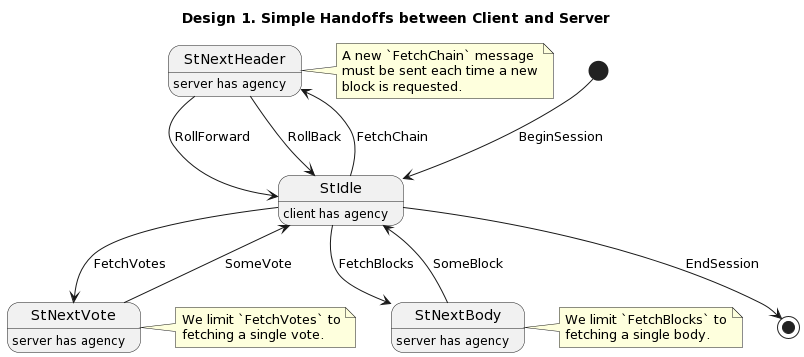
\includegraphics{../diagrams/sim-expts/protocol-1.png} &
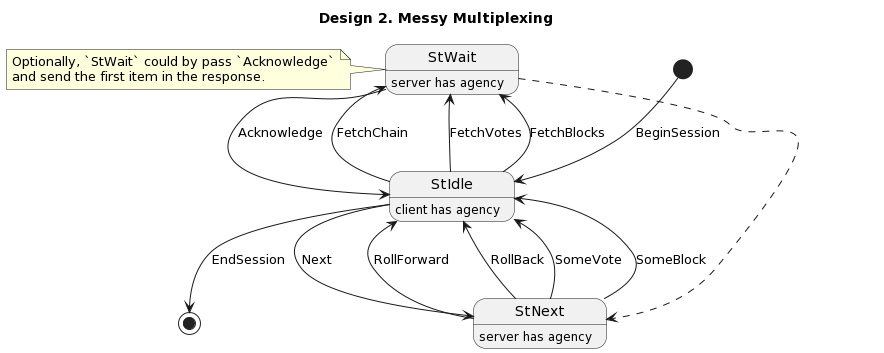
\includegraphics{../diagrams/sim-expts/protocol-2.png} &
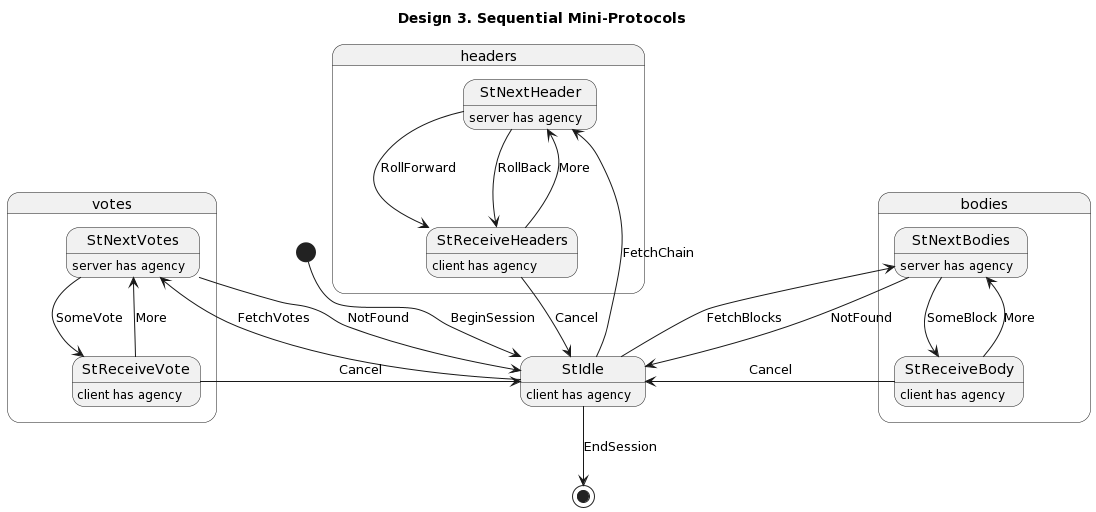
\includegraphics{../diagrams/sim-expts/protocol-3.png} &
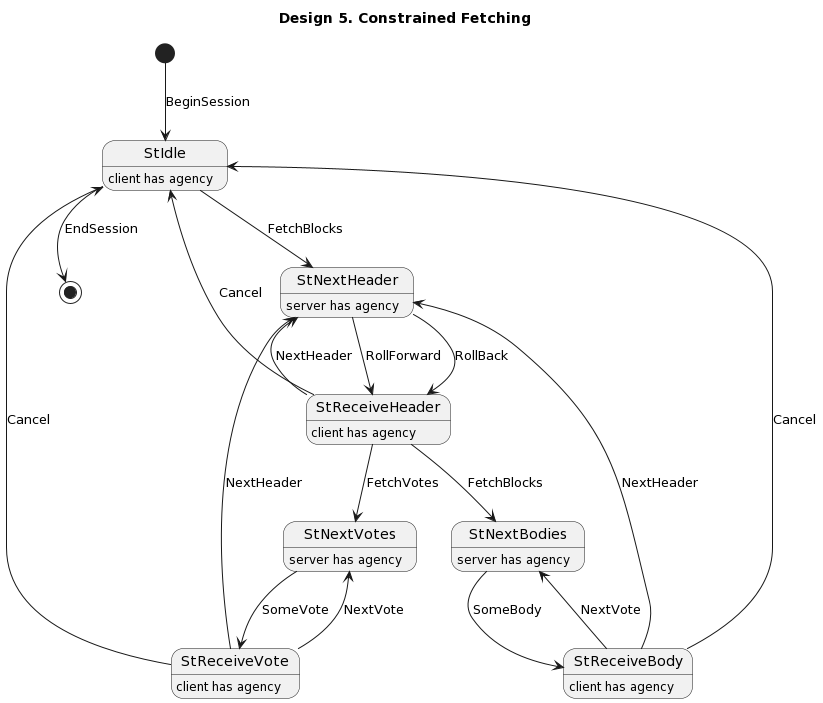
\includegraphics{../diagrams/sim-expts/protocol-5.png} \\
\end{longtable}

These highlight some key design issues:

\begin{itemize}
\tightlist
\item
  \texttt{FetchVotes} and \texttt{FetchBlocks} trigger multiple
  responses, as \texttt{FetchChain} may also do,
\item
  Three types of information are being queried (headers, votes, blocks)
  in only a semi-predictable sequence,
\item
  The DoS attack surface somewhat depends upon when the node yields
  agency to its peers,
\item
  Pull-based protocols involve more communication than push-based ones.
\end{itemize}

The current implementation uses a simple request/reply protocol that
avoids complexity, but is not explicitly defined as a state machine.
This is actually quite similar to the fifth design, but with no
\texttt{Next} request. It abandons the notion of when the client or
server has agency. If the client sends a new request before the stream
of responses to the previous request is complete, then responses will be
multiplexed.

\subsubsection{Experiments}\label{experiments}

The simulation experiments below use slightly different versions of the
ever-evolving Haskell package \texttt{peras-iosim}, which relies on the
types generated by \texttt{agda2hs}, but with the now slightly outdated
February version of the Peras protocol. Visualization was performed with
the \href{https://graphviz.org}{\color{blue}\texttt{GraphViz}} tool, and statistical and data
analysis was done with R.

\paragraph{Block production}\label{block-production}

The ``block production'' experiment laid the groundwork for testing
simulated block-production rates using QuickCheck properties. Because
the VRF determines which slots a node leads and forges a block, the
production is sporadic and pseudo-random. Heretofore, the Peras
simulation has used a simple probabilistic approximation to this
process: a uniformly distributed random variable is selected and the
node produces a block in the slot if that variable is less than the
probability \(p = 1 - (1 - f) ^ (s_\text{node} / s_\text{total})\),
where \$f is the active slot coefficient and \(s_\text{node}\) and
\(s_\text{total}\) are the stake held by the node and the whole network,
respectively.

The experiment involved running 1000 simulations of two hours of block
production for a node with \(\alpha = 0.05\). The stake held by the node
was randomly chosen in each of the simulations. The plot below shows the
number of blocks produced as a function of the node's stake. The
probability contours in the plot indicate the theoretical relationship.
For example, the 99.9\% quantile (indicated by 0.999 in the legend) is
expected to have only 1/1000 of the observations below it; similarly,
90\% of the observations should lie between the 5\% and 95\% contours.
The distribution of the number of blocks produced in the experiment
appears to obey the theoretical expectations.

\begin{figure}
\centering
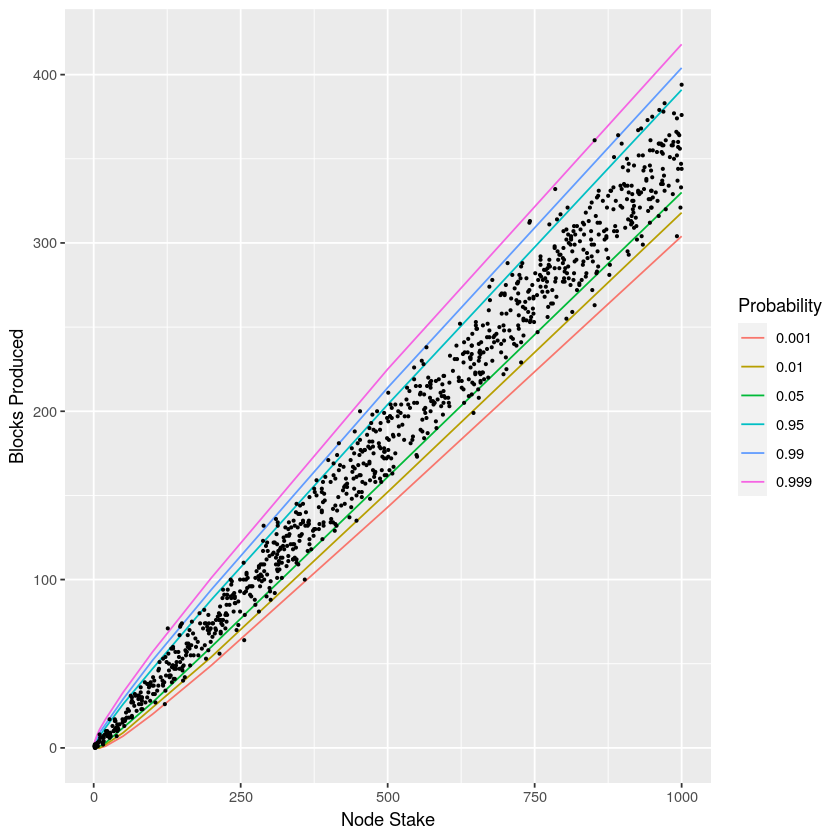
\includegraphics[width=0.58\textwidth]{../diagrams/sim-expts/blockproduction-scatter.png}
\caption{Relationship between a node's stake and the number of blocks it
produces}
\end{figure}

Although the above plot indicates qualitative agreement, it is somewhat
difficult to quantify the level of agreement because stake was varied in
the different simulations. The following histogram shows another view of
the same data, where the effect of different stake is removed by
applying the binomial cumulative probability distribution function (CDF)
for \(\alpha = 0.05\) to the data. Theoretically, this transformed
distribution should be uniform between zero and one. Once again, the
data appears to match expectations.

\begin{figure}
\centering
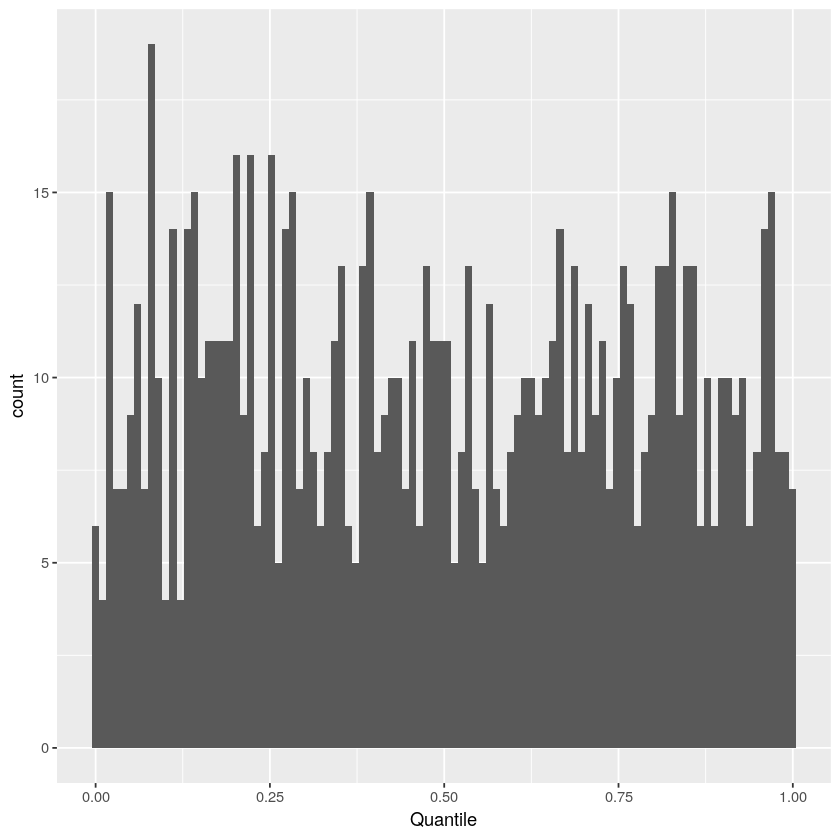
\includegraphics[width=0.58\textwidth]{../diagrams/sim-expts/blockproduction-quantiles.png}
\caption{Empirically observed quantiles of binomial distribution in
block-production experiment}
\end{figure}

A Kolmogorov-Smirnov (KS) test quantifies the conformance of the results
to such a uniform distribution:

\begin{Shaded}
\begin{Highlighting}[]
\FunctionTok{ks.test}\NormalTok{(results}\SpecialCharTok{$}\StringTok{\textasciigrave{}}\AttributeTok{Quantile}\StringTok{\textasciigrave{}}\NormalTok{, }\StringTok{"punif"}\NormalTok{, }\AttributeTok{min=}\DecValTok{0}\NormalTok{, }\AttributeTok{max=}\DecValTok{1}\NormalTok{)}
\end{Highlighting}
\end{Shaded}

\begin{Shaded}
\begin{Highlighting}[]
\NormalTok{D = 0.023265, p{-}value = 0.6587}
\NormalTok{alternative hypothesis: two{-}sided}
\end{Highlighting}
\end{Shaded}

The \emph{p}-value of 66\% solidly indicates that the block production
count matches our expectation and the theoretical model.

Because it is slightly inconvenient to embed a KS computation within a
QuickCheck property, one can instead use an approximation based on the
law of large numbers. The mean number of blocks produced in this
binomial process should be the number of slots times the probability of
producing a block in a slot, \(n p\), and the variance should be
\(n p (1-p)\). The \texttt{peras-quickcheck} module contains the
following function in \texttt{Data.Statistics.Util}:

\begin{Shaded}
\begin{Highlighting}[]
\CommentTok{{-}{-} | Check whether a value falls within the central portion of a binomial distribution.}
\OtherTok{equalsBinomialWithinTails ::}
  \CommentTok{{-}{-} | The sample size.}
  \DataTypeTok{Int} \OtherTok{{-}\textgreater{}}
  \CommentTok{{-}{-} | The binomial probability.}
  \DataTypeTok{Double} \OtherTok{{-}\textgreater{}}
  \CommentTok{{-}{-} | The number of sigmas that define the central acceptance portion.}
  \DataTypeTok{Double} \OtherTok{{-}\textgreater{}}
  \CommentTok{{-}{-} | The actual observation.}
  \DataTypeTok{Int} \OtherTok{{-}\textgreater{}}
  \CommentTok{{-}{-} | Whether the observation falls within the central region.}
  \DataTypeTok{Bool}
\end{Highlighting}
\end{Shaded}

The Peras continuous-integration tests are configured to require that
the observed number of blocks matches the theoretical value to within
three standard deviations. Practically, this means that the test
measurement is a random variable that will fall outside the three $\sigma$
range about once in every ten or so invocations of the CI (continuous
integration) tests, since each invocation executes 100 tests.

\paragraph{Network and Praos chain
generation}\label{network-and-praos-chain-generation}

The simulation experiments generate a reasonable but random topology of
peers, with a specified number of upstream and downstream nodes from
each node. Slot leadership is determined according to the procedure
outlined in the previous section above. Both the \texttt{peras-iosim}
Haskell package and the \texttt{peras\_topology} Rust package can
generate these randomized topologies and store them in YAML files. The
\texttt{peras-iosim} package generates valid Praos chains.

\begin{longtable}[]{@{}
  >{\raggedright\arraybackslash}p{(\columnwidth - 2\tabcolsep) * \real{0.4790}}
  >{\raggedright\arraybackslash}p{(\columnwidth - 2\tabcolsep) * \real{0.5210}}@{}}
\toprule\noalign{}
\begin{minipage}[b]{\linewidth}\raggedright
Example chain
\end{minipage} & \begin{minipage}[b]{\linewidth}\raggedright
Example topology
\end{minipage} \\
\midrule\noalign{}
\endhead
\bottomrule\noalign{}
\endlastfoot
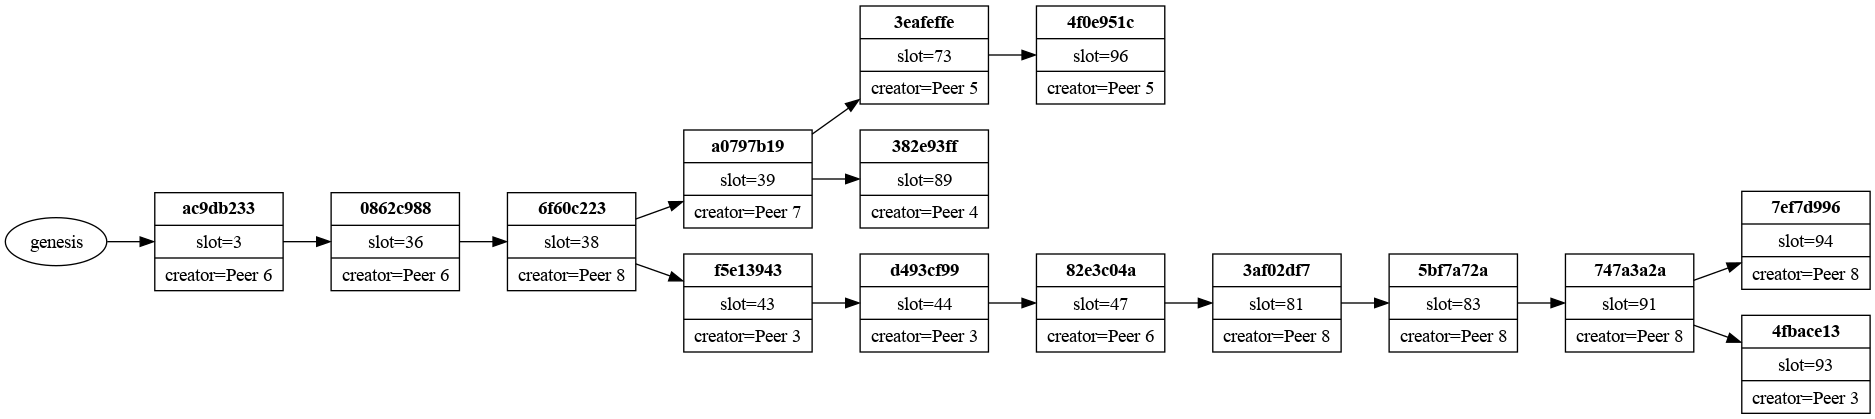
\includegraphics{../diagrams/sim-expts/example-chain.png} &
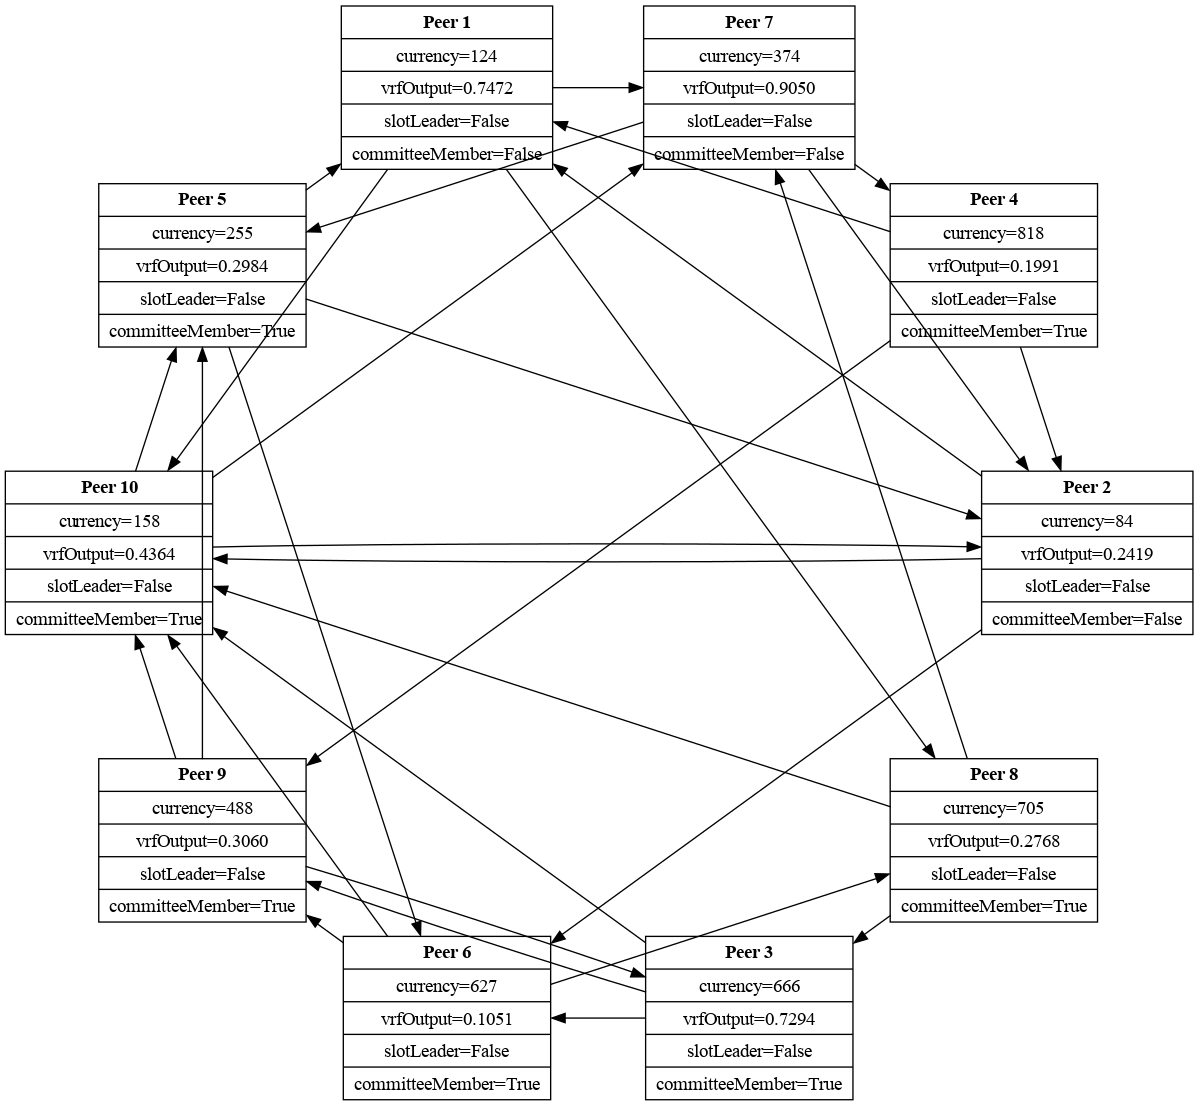
\includegraphics{../diagrams/sim-expts/example-network.png} \\
\end{longtable}

\paragraph{February version of Peras}\label{february-version-of-peras}

A semi-realistic set of protocol parameters and network configuration
was set for a 100-node network with a mean committee size of 10.
Committee selection in the following simulation was set by limiting each
node to a maximum of one vote. (However, the March version of the
protocol clarifies that a node may have more than one vote.) The
probability of becoming a member of the voting committee in a given
round is

\[
P = 1 - (1 - p_\text{lottery})^s
\]

given

\[
p_\text{lottery} = (1 - 1 / c)^{(c / t)}
\]

where \(s\) is the node's stake, \(t\) is the total stake in the system,
and \(c\) is the mean committee size.

The following figure compares similar Praos and Peras chains,
highlighting how the latter's voting boost affects the choice of
preferred chain. The simulation involved 100 nodes and a mean committee
size of 10 nodes; the active slot coefficient was set to 0.25 in order
to provoke more frequent forking than would normally be observed. The
voting boost is a modest 10\% per vote.

\begin{figure}
\centering
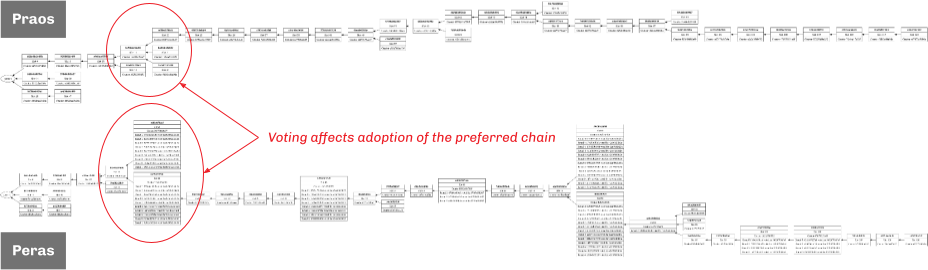
\includegraphics{../diagrams/sim-expts/peras-praos-comparison.png}
\caption{Comparison between Praos and Peras chains}
\end{figure}

The difference is fork adoption results from more Peras votes being
received by the lower chain than by the upper one, as illustrated below.

\begin{figure}
\centering
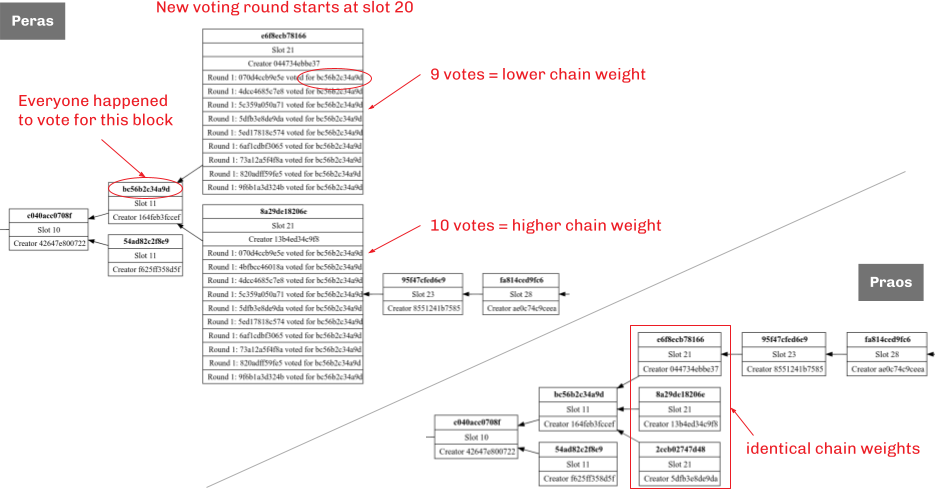
\includegraphics{../diagrams/sim-expts/peras-voting.png}
\caption{Detail of Peras and Praos chain comparison}
\end{figure}

Statistics for rollbacks, such as the ones shown below, are measured in
these simulations to quantify the number of slots or blocks that are
reverted: such can be used to compute the likelihood of a transaction
appearing in a block that is later rolled back. The diagram below shows
a proof-of-principle measurement of rollback lengths in an ensemble of
simulations. The horizontal axis shows the number of slots rolled back
during the course of the whole simulation, and the vertical axis shows
the corresponding number of blocks rolled back: the marginal histograms
show the empirically observed frequency of each. (Note that the point
indicating the number of slots vs blocks rolled back do not represent
single rollbacks of that many slots or blocks: instead a simulation
might have had many rollbacks and the slots and blocks listed are the
total among the rollbacks. Also note that the active slot coefficient
was set to a high value in order to provoke more forking.) Although the
voting boost weight is varied among these simulations, it has almost no
effect on the rollback statistics.

\begin{figure}
\centering
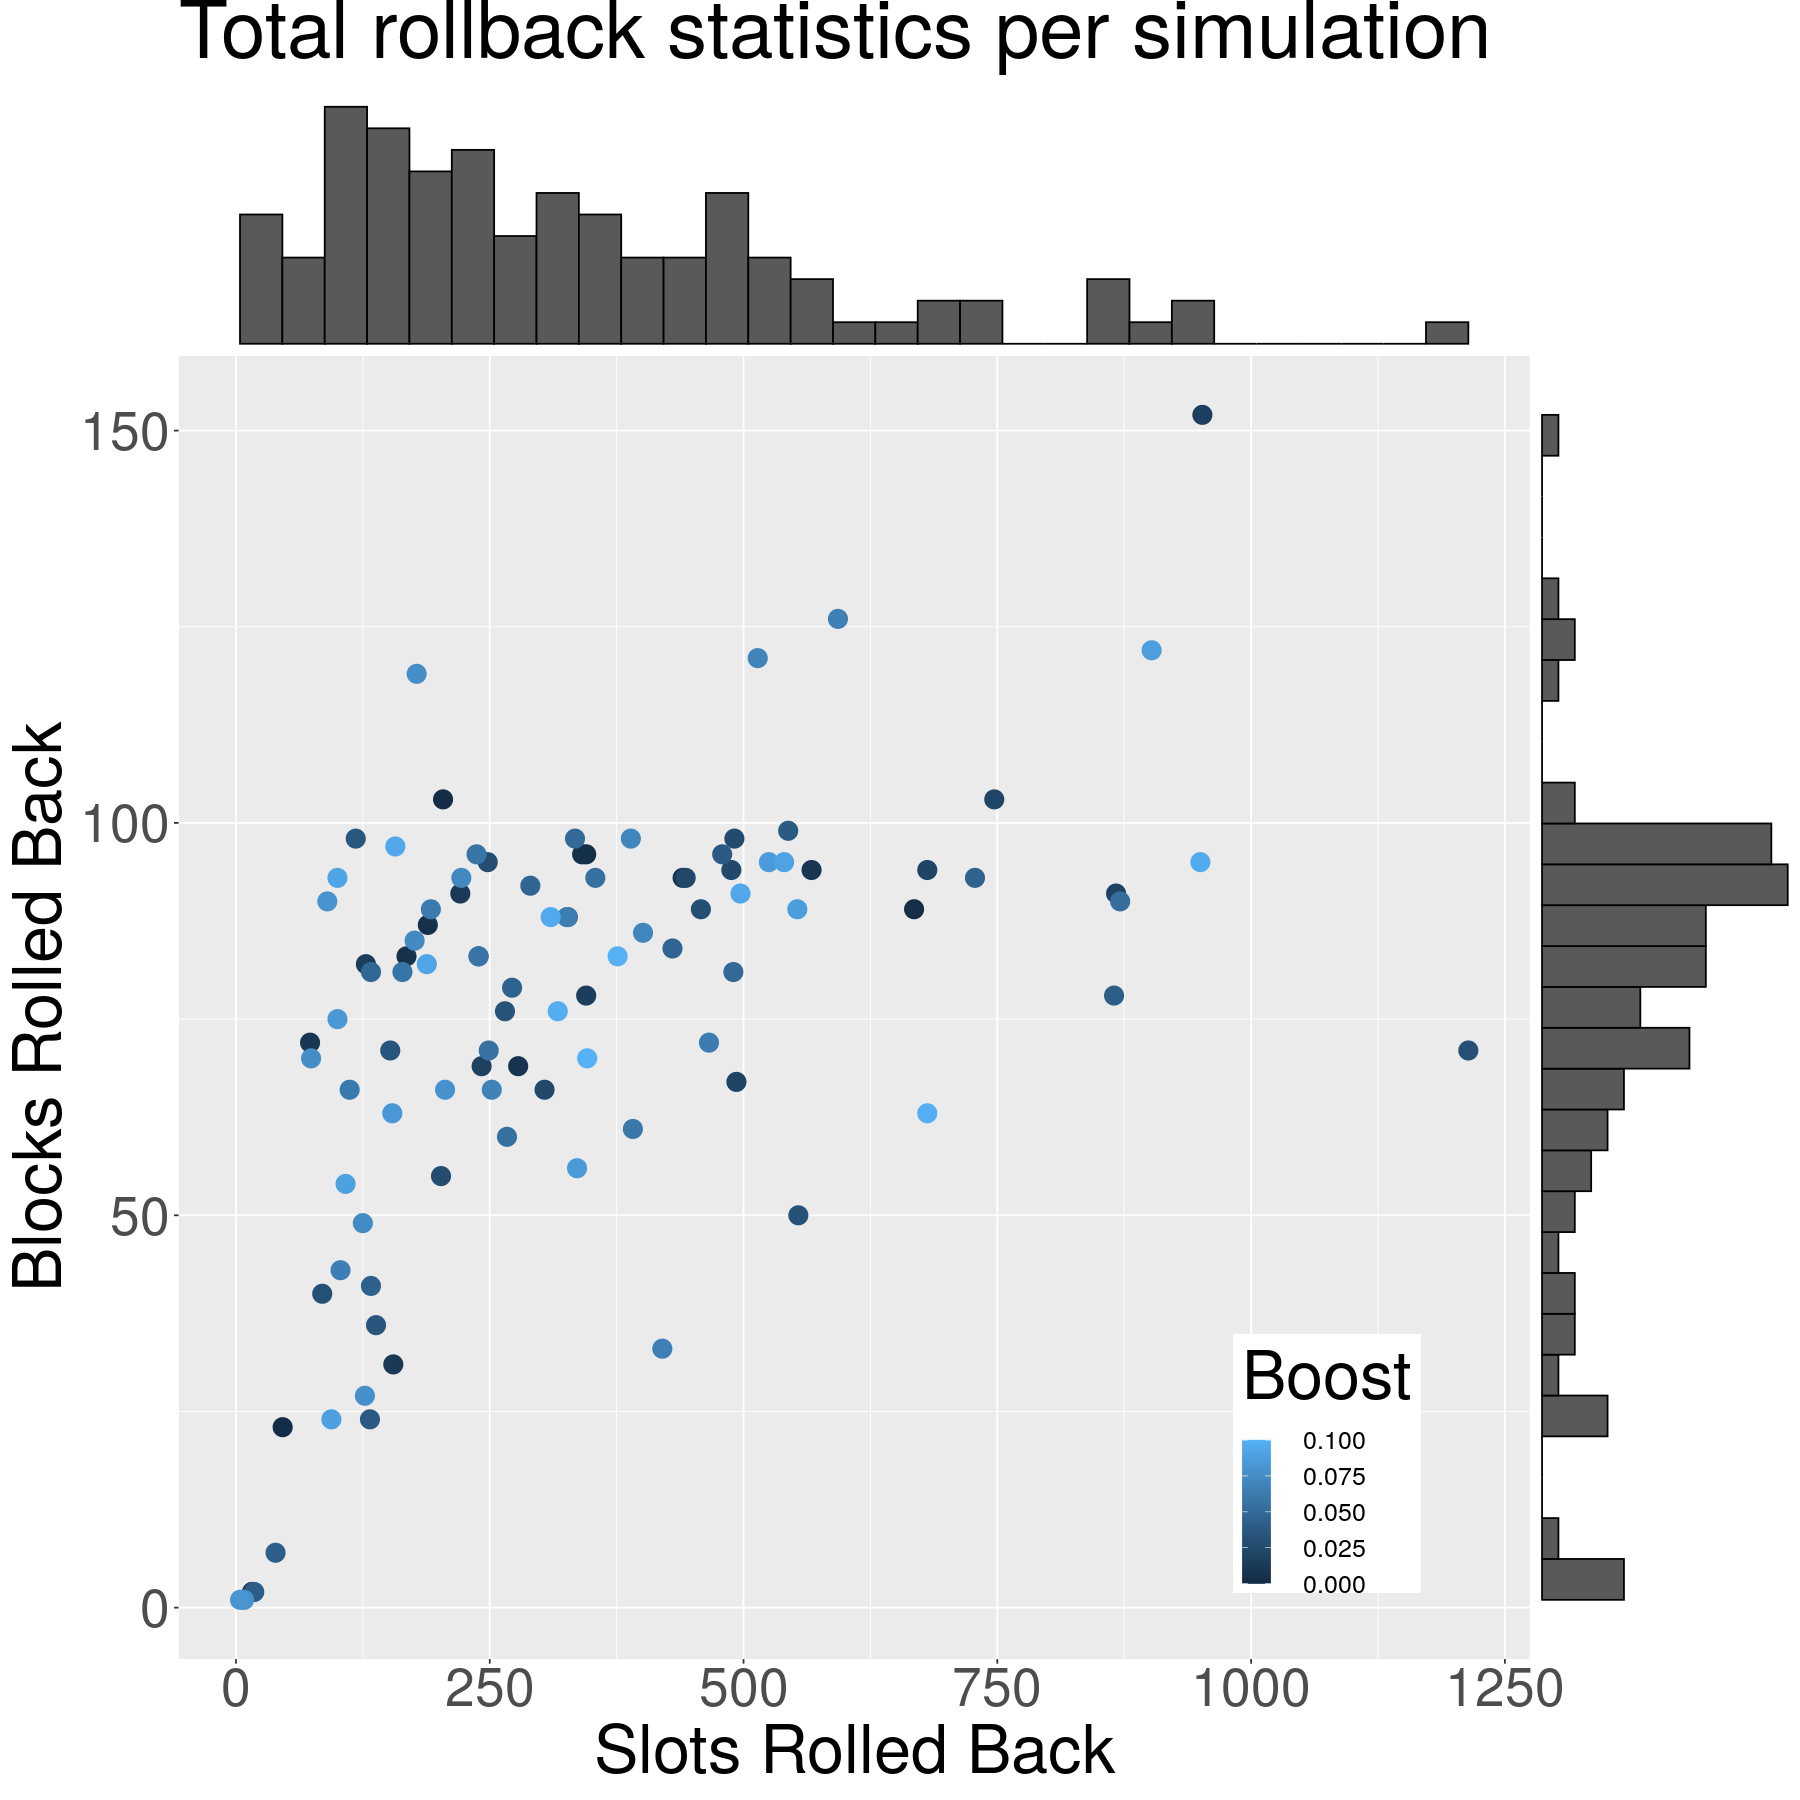
\includegraphics[width=0.58\textwidth]{../diagrams/sim-expts/rollbacks.png}
\caption{Example of rollback statistics}
\end{figure}

Findings from the simulation runs highlight the impracticality of
blindly running simulations with realistic parameters and then mining
the data:

\begin{itemize}
\tightlist
\item
  The simulation results are strongly dependent upon the speed of
  diffusion of messages through the network, so a moderately high
  fidelity model for that is required.
\item
  Both Peras and Praos are so stable that one would need very long
  simulations to observe naturally occurring forks of more than one or
  two blocks.

  \begin{itemize}
  \tightlist
  \item
    Only in cases of very sparse connectivity or slow message diffusion
    are longer forks seen.
  \item
    Peras quickly stabilizes the chain at the first block or two in each
    round, so even longer forks typically never last beyond then.
  \end{itemize}
\item
  Hence, even for honest nodes, one needs a mechanism to inject rare
  events such as multi-block forks, so that the effect of Peras can be
  studied efficiently.
\end{itemize}

\paragraph{``Split brain''}\label{split-brain}

This first ``split-brain'' experiment with \texttt{peras-iosim} involved
running a network of 100 nodes with fivefold connectivity for 15
minutes, but where nodes are partitioned into two non-communicating sets
between the 5th and 10th minute. The nodes quickly establish consensus
after genesis, but split into two long-lived forks after the 5th minute;
shortly after the 10th minute, one of the forks is abandoned as
consensus is reestablished.

Nodes were divided into two ``parities'' determined by whether the hash
of their name is an even or odd number. When the network is partitioned,
only nodes of the same parity are allowed to communicate with each
other: the Haskell module \texttt{Peras.IOSIM.Experiment.splitBrain}
implements the experiment and is readily extensible for defining
additional experiments.

Both the Praos and Peras protocols were simulated, with the following
Peras parameters for creating a scenario that exhibits occasional
cool-down periods and a strong influence of the voting boost.

\begin{Shaded}
\begin{Highlighting}[]

\FunctionTok{activeSlotCoefficient}\KeywordTok{:}\AttributeTok{ }\FloatTok{0.10}
\FunctionTok{roundDuration}\KeywordTok{:}\AttributeTok{ }\DecValTok{50}
\FunctionTok{pCommitteeLottery}\KeywordTok{:}\AttributeTok{ }\FloatTok{0.00021}
\FunctionTok{votingBoost}\KeywordTok{:}\AttributeTok{ }\FloatTok{0.25}
\FunctionTok{votingWindow}\KeywordTok{:}\AttributeTok{ }\KeywordTok{[}\DecValTok{150}\KeywordTok{,}\AttributeTok{ }\DecValTok{1}\KeywordTok{]}
\FunctionTok{votingQuorum}\KeywordTok{:}\AttributeTok{ }\DecValTok{7}
\FunctionTok{voteMaximumAge}\KeywordTok{:}\AttributeTok{ }\DecValTok{100}
\FunctionTok{cooldownDuration}\KeywordTok{:}\AttributeTok{ }\DecValTok{4}
\FunctionTok{prefixCutoffWeight}\KeywordTok{:}\AttributeTok{  }\DecValTok{10000000}
\end{Highlighting}
\end{Shaded}

The control (``normal'') case is a network that does not experience
partitioning:

\begin{Shaded}
\begin{Highlighting}[]
\FunctionTok{randomSeed}\KeywordTok{:}\AttributeTok{ }\DecValTok{13234}
\FunctionTok{peerCount}\KeywordTok{:}\AttributeTok{ }\DecValTok{100}
\FunctionTok{downstreamCount}\KeywordTok{:}\AttributeTok{ }\DecValTok{5}
\FunctionTok{maximumStake}\KeywordTok{:}\AttributeTok{ }\DecValTok{1000}
\FunctionTok{messageDelay}\KeywordTok{:}\AttributeTok{ }\DecValTok{350000}
\FunctionTok{endSlot}\KeywordTok{:}\AttributeTok{ }\DecValTok{1500}
\FunctionTok{experiment}\KeywordTok{:}
\AttributeTok{  }\FunctionTok{tag}\KeywordTok{:}\AttributeTok{ NoExperiment}
\end{Highlighting}
\end{Shaded}

The treatment (``split'') case experiences partitioning between the 5th
and 10th minutes:

\begin{Shaded}
\begin{Highlighting}[]
\FunctionTok{randomSeed}\KeywordTok{:}\AttributeTok{ }\DecValTok{13234}
\FunctionTok{peerCount}\KeywordTok{:}\AttributeTok{ }\DecValTok{100}
\FunctionTok{downstreamCount}\KeywordTok{:}\AttributeTok{ }\DecValTok{5}
\FunctionTok{maximumStake}\KeywordTok{:}\AttributeTok{ }\DecValTok{1000}
\FunctionTok{messageDelay}\KeywordTok{:}\AttributeTok{ }\DecValTok{350000}
\FunctionTok{endSlot}\KeywordTok{:}\AttributeTok{ }\DecValTok{1500}
\FunctionTok{experiment}\KeywordTok{:}
\AttributeTok{  }\FunctionTok{tag}\KeywordTok{:}\AttributeTok{ SplitBrain}
\AttributeTok{  }\FunctionTok{experimentStart}\KeywordTok{:}\AttributeTok{ }\DecValTok{500}
\AttributeTok{  }\FunctionTok{experimentFinish}\KeywordTok{:}\AttributeTok{ }\DecValTok{1000}
\end{Highlighting}
\end{Shaded}

In the Peras simulation, the chain that eventually became dominant
forged fewer blocks during the partition period, but it was lucky to
include sufficient votes for a quorum at slot 503 and that kept the
chain out of the cool-down period long enough to put more votes on the
chain, which increased the chain weight. It appears that that was
sufficient for the chain to eventually dominate. Note that multiple
small forks occurred between the time that network connectivity was
restored and consensus was reestablished.

\begin{figure}
\centering

\includegraphics{../diagrams/sim-expts/split-brain.png}
\caption{Forking and reestablishment of quorum in Peras split-brain
experiment}
\end{figure}

The primary measurements related to the loss and reestablishment of
consensus relate to the length of the forks, measured in blocks or
slots. The table shows the statistics of these forks, of which the Peras
case had several.

\begin{longtable}[]{@{}
  >{\raggedright\arraybackslash}p{(\columnwidth - 6\tabcolsep) * \real{0.1282}}
  >{\raggedright\arraybackslash}p{(\columnwidth - 6\tabcolsep) * \real{0.6795}}
  >{\raggedleft\arraybackslash}p{(\columnwidth - 6\tabcolsep) * \real{0.1026}}
  >{\raggedleft\arraybackslash}p{(\columnwidth - 6\tabcolsep) * \real{0.0897}}@{}}
\toprule\noalign{}
\begin{minipage}[b]{\linewidth}\raggedright
Protocol
\end{minipage} & \begin{minipage}[b]{\linewidth}\raggedright
Metric
\end{minipage} & \begin{minipage}[b]{\linewidth}\raggedleft
Blocks
\end{minipage} & \begin{minipage}[b]{\linewidth}\raggedleft
Slots
\end{minipage} \\
\midrule\noalign{}
\endhead
\bottomrule\noalign{}
\endlastfoot
Praos & Length of discarded chain at slot 1000 & 68 & 1000 \\
& Length of dominant chain at slot 1000 & 73 & 1000 \\
& Number of blocks in discarded chain after slot 1000 & 2 & \\
Peras & Length of discarded chain at slot 1000 & 75 & 1000 \\
& Length of dominant chain at slot 1000 & 66 & 1000 \\
& Number of blocks in discarded chain after slot 1000 & 3 & 137 \\
& & 1 & 118 \\
& & 1 & 137 \\
& & 1 & 141 \\
& & 1 & 55 \\
& & 1 & 24 \\
& & 1 & 18 \\
& Number of blocks afters slot 1000 to reach quorum & 18 & 304 \\
\end{longtable}

The primary findings from this experiment follow.

\begin{itemize}
\tightlist
\item
  The complexity of the forking, voting, and cool-down in the Peras
  results highlights the need for capable visualization and analysis
  tools.
\item
  The voting boost can impede the reestablishment of consensus after a
  network partition is restored.
\item
  It would be convenient to be able to start a simulation from an
  existing chain, instead of from genesis.
\item
  VRF-based randomization makes it easier to compare simulations with
  different parameters.
\item
  Even though \texttt{peras-iosim} runs are not particularly fast, one
  probably does not need to parallelize them because typical experiments
  involve many executions of simulations, which means we can take
  advantage of CPU resources simply by running those different scenarios
  in parallel.
\item
  The memory footprint of \texttt{peras-iosim} is small (less than 100
  MB) if tracing is turned off; with tracing, it is about twenty times
  that, but still modest.
\end{itemize}

\paragraph{Congestion}\label{congestion}

A coarse study exercised several aspects of \texttt{peras-iosim} in a
simulation experiment involving network congestion: simulation/analysis
workflow, scalability and performance, and observability. A full
factorial experiment varied bandwidth and latency on a small network
with semi-realistic Peras parameters. Each block has its maximum size:
i.e., each block is completely full of transactions. There were 250
nodes with fivefold connectivity and a mean of 25 committee members;
latency varied from 0.25 s to 1.00 s, and bandwidth varied from 8 Mb/s
to 400 Mb/s, but other parameters remained constant.

The main caveat is that the memory pool and other non-block/non-vote
messages were not modeled. Several findings were garnered from this
experiment:

\begin{itemize}
\tightlist
\item
  A threshold is readily detectable at a bandwidth of \textasciitilde20
  Mb/s.

  \begin{itemize}
  \tightlist
  \item
    It is important to realize that this simulation was neither
    calibrated to realistic conditions nor validated.
  \item
    Much better empirical data inputs for on node processing times
    (e.g., signature verification, block assembly, etc.) are needed.
  \end{itemize}
\item
  Non-block and not-vote messages such as those related to the memory
  pool must be accounted for in congestion.
\item
  The existing \texttt{peras-iosim} event logging and statistics system
  easily supports analyses such as these.
\end{itemize}

The following diagram shows the cumulative bytes received by nodes as a
function of network latency and bandwidth, illustrating the threshold
below which bandwidth is saturated by the protocol and block/vote
diffusion.

\begin{figure}
\centering
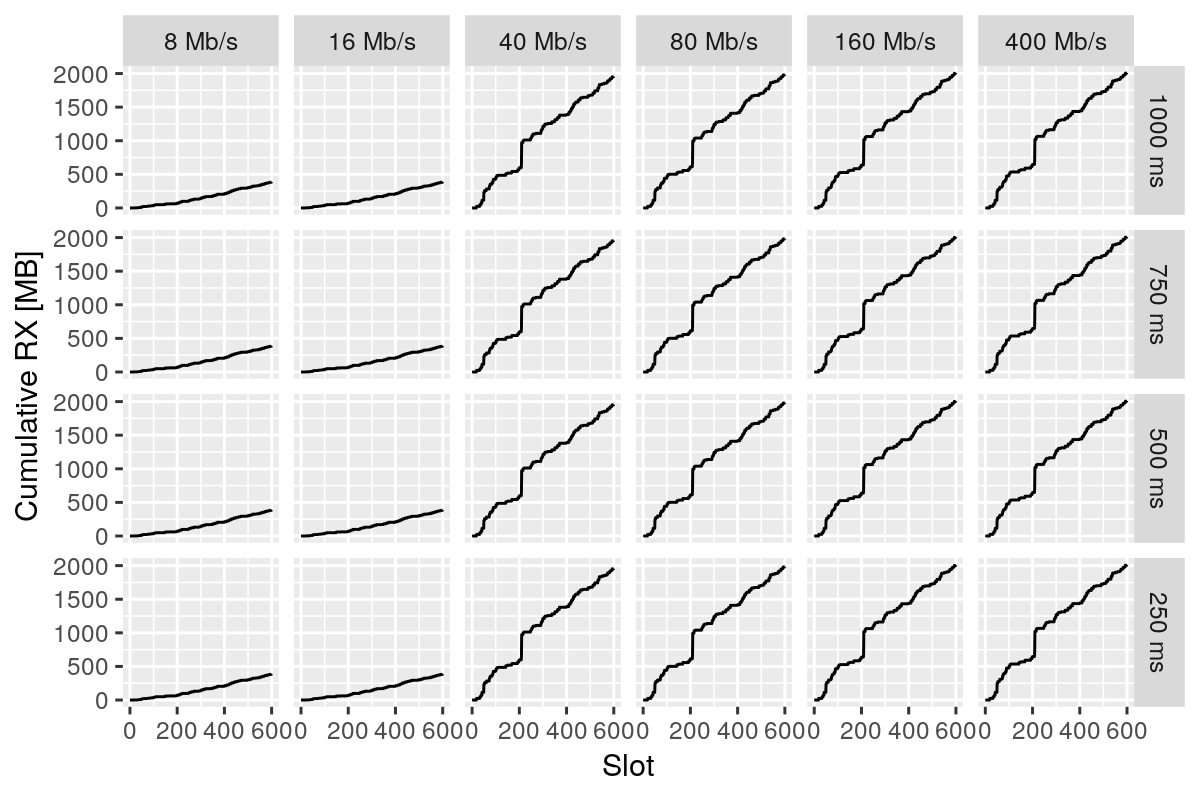
\includegraphics{../diagrams/sim-expts/congestion.png}
\caption{Cumulative bytes received by nodes as a function of network
latency and bandwidth}
\end{figure}

\subsection{Rust-based simulation}\label{rust-based-simulation}

The Rust types for Peras nodes and networks mimic the Haskell ones and
the messages conform to the Agda-generated types. The Rust
implementation demonstrates the feasibility of using
language-independent serialization and a foreign-function interface
(FFI) for Haskell-based QuickCheck testing of Peras implementations. In
particular, the Rust package \texttt{serde} has sufficiently
configurable serialization so that it interoperates with the default
Haskell serializations provided by \texttt{Data.Aeson}. (The new
\texttt{agda2rust} tool has not yet reached a stable release, but it may
eventually open possibilities for generating Rust code from the Agda
types and specification.) A Rust static library can be linked into
Haskell code via Cabal configuration.

The Rust node generates Praos blocks according to the slot-leadership
recipe. The Rust network uses the Innovation Team's new network
simulation
\href{https://github.com/input-output-hk/ce-netsim}{\color{blue}\texttt{ce-netsim}} for
transportation block-production and preferred-chain messages among the
nodes.

The key findings from Rust experiments follow.

\begin{itemize}
\tightlist
\item
  It is eminently practical to interface non-Haskell code to QuickCheck
  Dynamic via language-independent serialization and a foreign-function
  interface.
\item
  It is also possible to co-design Rust and Haskell code for Peras so
  that the implementations mirror each other, aside from
  language-specific constructs. This might result in not employing the
  advanced and idiosyncratic features of these two languages, however.
\item
  The \texttt{ce-netsim} architecture and threading model is compatible
  with Peras simulations, even ones linked to
  \texttt{quickcheck-dynamic} test via FFI.
\end{itemize}

\subsection{Overall findings from simulation
studies}\label{overall-findings-from-simulation-studies}

\subsubsection{Simulation results}\label{simulation-results}

\begin{itemize}
\tightlist
\item
  Both Peras and Praos are so stable that one would need very long
  simulations to observe forks of more than one or two blocks.

  \begin{itemize}
  \tightlist
  \item
    Only in cases of very sparse connectivity or slow message diffusion
    are longer forks seen in honest networks.
  \item
    Peras quickly stabilizes the chain at the first block or two in each
    round, so even longer forks typically never last beyond then.
  \item
    Hence, even for honest nodes, we need a mechanism to inject rare
    events such as multi-block forks, so that the effect of Peras can be
    studied efficiently.
  \end{itemize}
\item
  The voting boost can impede the reestablishment of consensus after a
  network partition is restored.
\item
  The simulation results are strongly dependent upon the speed of
  diffusion of messages through the network, so a moderately high
  fidelity model for that is required.
\item
  Congesting experiments can detect when vote-related messages impact
  node performance.
\end{itemize}

\subsubsection{Simulation experiments}\label{simulation-experiments}

\begin{itemize}
\tightlist
\item
  Single-threaded simulations of 1000s of nodes for one or more
  simulated days are feasible.
\item
  The parameter space is large enough (approximately ten dimensions)
  that statistically designed experiments (latin hypercubes, orthogonal
  arrays, or hybrids) and importance sampling will be needed to focus
  computational resources on the performance regimes of most interest.
\item
  Finely crafted, demonstrative simulation scenarios are needed for
  highlighting the value added by Peras.
\item
  The complexity of the forking, voting, and cool-down in the Peras
  results highlights the need for capable visualization and analysis
  tools.
\item
  More data on CPU usage for various node activities (verifying
  signatures, forging blocks, etc.) is needed for realistic simulation
  of node resource usage.

  \begin{itemize}
  \tightlist
  \item
    The performance reports being prepared for the Conway era have some
    of this information, but it is not quite at the granularity needed
    for a simulation.
  \end{itemize}
\end{itemize}

\subsubsection{Simulator design}\label{simulator-design}

\begin{itemize}
\tightlist
\item
  There is little point in expending the extra effort to develop
  multi-threaded, parallel network simulations because CPU resources
  could instead be devoted to the large ensembles of simulations that
  will be needed for some studies.

  \begin{itemize}
  \tightlist
  \item
    Furthermore, the Ouroboros security parameter of 2160 blocks limits
    the duration of interesting simulations.
  \item
    However, A conservative parallel discrete event is feasible to
    implement if higher performance is needed for the simulation
    studies.
  \end{itemize}
\item
  Congestion modeling may require representing all message traffic
  between nodes (not just blocks, votes, and certificates).

  \begin{itemize}
  \tightlist
  \item
    However, the March version of the Peras protocol imposes a far
    lighter network load than the February version.
  \item
    Hence, analytic estimates or ΔQ analyses may be sufficient for
    assessing the message-traffic overhead resulting from Peras.
  \end{itemize}
\item
  It would be convenient to be able to start a simulation from an
  existing chain, instead of from genesis.
\item
  Non-block and not-vote messages such as those related to the memory
  pool must be accounted for in congestion.
\item
  The following detail for event logging is sufficient for analysis and
  visualization of the simulations.

  \begin{itemize}
  \tightlist
  \item
    CPU resource consumption.
  \item
    Bytes transmitted and received.
  \item
    Slot leadership and committee membership.
  \item
    Occurrence of rollbacks.
  \item
    The sending, receiving, and dropping of messages.
  \end{itemize}
\item
  Language-independent schemas (in YAML or JSON) for scenario
  definition, network topology, observability, and visualization create
  seamless interoperability between Haskell and Rust simulators.

  \begin{itemize}
  \tightlist
  \item
    Query tools such as \texttt{jq} and \texttt{mongo} work well for
    ad-hoc analysis of the event logs.
  \item
    Log analysis and visualization tools can be compatible with Peras
    observability.
  \end{itemize}
\item
  Haskell

  \begin{itemize}
  \tightlist
  \item
    The \texttt{agda2hs} tool generates Haskell that is usable in
    simulations and QuickCheck.

    \begin{itemize}
    \tightlist
    \item
      The biggest awkwardness is that one has to write some orphan
      instances (including \texttt{Arbitrary}) in Haskell instead of in
      Agda.
    \end{itemize}
  \item
    Keeping the exported Haskell implementation ``boring'' (i.e.,
    avoiding type-level machinery, complex monad transformer stacks, no
    STM, etc.) facilitates its interoperability with
    \texttt{quickcheck-dynamic} and language-independent APIs.
  \item
    An efficient Haskell simulation requires auxiliary data structures
    to index the blocks, votes, and certificates in the block tree, to
    memoize quorum checks, etc.
  \end{itemize}
\item
  Rust

  \begin{itemize}
  \tightlist
  \item
    The \texttt{serde} Rust libraries successfully mimic Haskell's
    \texttt{aeson} serialization for JSON.
  \item
    The \texttt{serde} library also supports serialization as CBOR,
    though its compatibility with Cardano's CBOR serialization has not
    yet been assessed.
  \item
    The \texttt{agda2rust} tool is not sufficiently mature to generate
    Peras's Agda types for use in Rust.
  \item
    The \texttt{ce-netsim} library is useful for the message-passing
    portions of Peras simulations written in Rust.
  \item
    Using WASM as a Rust compilation target may enable running
    serverless simulations in a web browser.
  \end{itemize}
\item
  IOSim

  \begin{itemize}
  \tightlist
  \item
    IOSim's single-threaded implementation hinders its usefulness for
    high performance simulations.
  \item
    It is quite awkward to use random numbers (e.g.,
    \texttt{StatefulGen}) within \texttt{IOSim} because it lacks the
    requisite monad-transformer instances. The experimental and outdated
    \texttt{io-classes-mtl} package does not solve this problem.
  \end{itemize}
\item
  QuickCheck

  \begin{itemize}
  \tightlist
  \item
    Some tests of node behavior may be statistical, but the current
    codebase demonstrates how properties that only hold statistically
    can be incorporated into continuous-integration (CI) tests.
  \end{itemize}
\item
  Ideally, simulation analysis and visualization tools could be
  browser-based, so that stakeholders could explore Peras and build
  intuition about it without installing any software.
\end{itemize}

\subsubsection{Integration with QuickCheck
Dynamic}\label{integration-with-quickcheck-dynamic}

Now that it has been demonstrated that it is feasible to export Agda
types, functions, and QuickCheck dynamic models to Haskell for testing,
an optimal path forward would be to have those generated types dictate
the public interfaces for node and network simulations (both in Haskell
and in Rust). The current simulation codebase is consistent with this
test-driven development (TDD) approach and will only require minor
adjustments to yield simulations that are faithful to Peras and that are
primarily based on exported Agda types and functions. The same
simulation implementation will both conform to the
\texttt{quickcheck-dynamic} models and the requirement for efficient
simulation.

\section{Integration into Cardano
Node}\label{integration-into-cardano-node}

This section studies the required work and potential impacts of
implementing Peras as a core component of the Cardano node. The main
impacts identified are that:

\begin{itemize}
\tightlist
\item
  Peras requires significant changes to message traffic between nodes,
  with new types of messages and network protocols,
\item
  It \emph{might} require changes to the structure of blocks,
\item
  It increases the computational resources used by nodes through the
  need to produce and validate votes.
\end{itemize}

\subsection{Networking}\label{networking}

Peras introduces two new constructs: votes and certificates. Members of
the Peras committee cast votes each voting round, and the votes must be
received by a block-producing node before the votes expire. A
certificate memorializes a quorum of votes (approximately 80\% of the
committee) made in the same round for a particular block. A certificate
must be included in the first block of a cool-down period, though at
least one variant of the protocol envisions each round's certificate
being included regardless of cool-down status. Nodes syncing from
genesis or an earlier point in the chain's history must be provided the
votes or equivalent certificates in order for them to verify the weight
of the chain. Thus, the protocol results in the following message
traffic:

\subsubsection{Votes}\label{votes}

\begin{itemize}
\tightlist
\item
  Vote messages diffuse votes from voters to the block-producing nodes.

  \begin{itemize}
  \tightlist
  \item
    An upper bound (worst-case scenario) on message traffic is that
    every vote diffuses to every node.
  \item
    Votes would likely be sent via a new mini-protocol very similar to
    how transactions are propagated:

    \begin{itemize}
    \tightlist
    \item
      The downstream peers request list of IDs from upstream peers
    \item
      They select the ones they do not have in their ``mempools'' for
      download
    \item
      When quorum is reached they stop downloading votes for given round
    \end{itemize}
  \item
    Backpressure for a node's receiving is necessary in order to
    mitigate DoS attacks that flood a node with votes.
  \item
    Nodes that have large stake might be allotted several votes. Instead
    of sending one message per vote, these could be bundled as a message
    that indicates the number of votes cast.
  \item
    Votes not recorded on the chain or in a certificate need to be kept
    by the node and persistently cached if the node is restarted. They
    might have to be provided to newly syncing nodes.
  \end{itemize}
\item
  It is relatively straightforward to know the size the votes mempool
  would take

  \begin{itemize}
  \tightlist
  \item
    The size of a vote is likely a couple of hundred bytes.
  \item
    Votes have a TTL (parameter max. age \(A\) of the protocol) which
    implies there is a strict upper bound on the overall size of the
    votes mempool
  \item
    There is also a cap on the number of votes per round (quorum
    parameter \(\tau\))
  \item
    And it is always possible to trade a bunch of votes with a
    certificate representing those votes
  \end{itemize}
\end{itemize}

\subsubsection{Certificates}\label{certificates-1}

Certificates (or equivalently quorum of votes in a round) have an impact
on the chain selection process as they change the weight:

\begin{itemize}
\tightlist
\item
  Sending a certificate is equivalent to sending a quorum of votes.

  \begin{itemize}
  \tightlist
  \item
    Once a node sees a quorum, it can create and diffuse a certificate
    so it no longer needs to send any more votes for the round.
  \item
    If non-quorum certificates were to obey monoid laws, then votes
    could be sent as singleton certificates that progressively aggregate
    votes towards a quorum. This use of non-quorum certificates would
    reduce message traffic.
  \item
    If a certificate for every round is included on the chain, then
    newly started or syncing nodes need not request certificates or
    votes for rounds older than the last certificate recorded on the
    chain.
  \item
    Certificates not recorded on the chain need to be kept by the node
    and persistently cached in case the node is restarted. They might
    have to be provided to newly syncing nodes.
  \item
    The size of a certificate is likely a few thousand bytes or more
  \item
    Conceptually, diffusion of certificates can be thought as similar to
    the diffusion of blocks as certificates are explicitly or implicitly
    chained together
  \end{itemize}
\item
  Certificates are likely too large to be included in the block header
  without increasing its size over the constitutionally-constrained byte
  limit.

  \begin{itemize}
  \tightlist
  \item
    If the CDDL for blocks were altered, they could be included as a new
    entry in the block.
  \item
    Alternatively, a certificate could be stored as a transaction in the
    block. Such certificate-transactions would incur a fee and would
    also need to be prioritized ahead of transactions in the memory
    pool.
  \end{itemize}
\item
  At least conceptually, certificates are \emph{fungible}: e.g.~if I
  have certificate X for block A and a certificate Y for block B s.t. A
  extends B, then I can count the chain from B as having twice the
  weight which is equivalent to having a certificate \(Z = X \circ Y\).

  \begin{itemize}
  \tightlist
  \item
    This implies that an implementation could choose to merge
    certificates that are past some threshold, e.g.~when enough weight
    has been accumulated the chances of chain fork are negligible, which
    would limit the storage requirements.
  \item
    This needs to be validated by researchers and is highly dependent on
    the particular technology used to form certificates.
  \end{itemize}
\item
  Creating, and to a lesser extent validating, certificates could be
  relatively CPU intensive operations.

  \begin{itemize}
  \tightlist
  \item
    This means there is an interesting operational tradeoff between
    resources, CPU on one hand, and memory/network bandwidth on the
    other, that could be used by an implementation adaptively depending
    on the environment's conditions: Share quorum of votes directly if
    there is no pressure on memory and network bandwidth, or spend CPU
    time to build certificates to reduce footprint.
  \end{itemize}
\end{itemize}

\subsection{Consensus}\label{consensus}

The node's chain-selection algorithm will have to be modified to compute
chain weight that includes the boosts from the certificates on the
chain. It will also have to do bookkeeping on unrecorded votes and
certificates and adjust the relevant data structures when a new
preferred chain is selected.

\subsection{Resources}\label{resources}

Peras requires several new types of work by the node: votes and
certificates must be created, diffused, persistently cached, and
verified. CPU resources for creating a vote are on the order of those
used by creating a signature. Verifying a vote likely will use resources
similar to verifying the slot leadership of another node, since a
similar VRF scheme is used for both voting and slot leadership.
Resources for creating or verifying a certificate will depend upon the
particular certification scheme selected, for example Approximate Lower
Bounds. The burden of verifying votes might be lessened if the
certificates containing them can be built incrementally and forwarded to
downstream peers which will not have to re-verify the votes.

If certificates for each round are not stored permanently on the chain,
then they will have to be persisted locally by each node. This has the
drawback of making it impossible to verify the evolution of the chain
without having the off-chain information about certificates.

\subsection{Implementation path}\label{implementation-path}

The somewhat nice decoupling between the voting layer and the Nakamoto
consensus layer, along with the fact that votes are only taken into
account in bulk, e.g.~when they form a quorum on some round, seems to
make it possible to implement Peras in a way that does not impact too
much consensus, and at very least in an incremental way.

\begin{itemize}
\tightlist
\item
  It might be possible to experiment with Peras using real nodes on a
  special-purpose testnet. Votes and certificates could be represented
  as ordinary transactions with well-known characteristics. A thread
  could be added to the node to create and verify votes and
  certificates. The node's chain-selection code would have to
  communicate with that thread.
\item
  A dedicated votes and certificate management process could be built
  and run separately, with the node only periodically checking this
  process when it needs to decide upon chain selection. While this might
  not be acceptable on a real production network due to the added
  latency on a critical path, it might be good enough to experiment with
  Peras on a testnet.
\item
  The network protocol for diffusing votes bears a lot of similarity to
  the kind of network needed by
  \href{https://hackmd.io/jwAdFPzZQj-llwfavl8Ahw}{\color{blue}\texttt{Mithril}} on its path
  to increased decentralization, so the effort to develop those
  protocols could be shared.
\end{itemize}

\newpage

\section{Conclusion}\label{conclusion-1}

The analyses described in this report provides some evidence that the
Peras protocol could be a viable addition to the Cardano blockchain, in
that it would significantly speed settlement (or, more precisely,
rapidly decrease settlement-failure probabilities) without burdening the
nodes with substantial additional computational or bandwidth
requirements. Feedback regarding early versions of the Peras protocol,
which was untenable for efficient implementation, resulted in minor
adjustments to the protocol which seem to make it more practical for
deployment. The analyses were achieved via a combined program of
formalization in Agda, network modeling using the ΔQ methodology,
message-passing simulations in Haskell and Rust, and dynamic QuickCheck
testing. An important byproduct of this work was the formulation and
demonstration of a potentially reusable methodology that delivers a
formal specification that is closely tied to a chain of evidence
involving modeling, simulation, and conformance testing.

The foregoing analyses have quantified and reduced several risks related
to adoption of Peras. In particular, the number and size of vote and
certificate messages passing between nodes would not significantly
impact a node's performance or tax its bandwidth. Similarly, the size of
the block headers would not be impacted by Peras, though some block
bodies (one per voting round) would be several hundred bytes longer to
accommodate a certificate that attests to a voting quorum having been
achieved. The chain weight can be verified externally by examining the
history of certificates attached to blocks, but following the current
best chain would require a knowledge of the votes or certificates that
had not yet been memorialized by inclusion of a certificate in a block:
nodes would have to persistently cache such information, which would
only require negligible memory and disk space. Vote and certificate
processing have some temporal flexibility, so their resource usage can
be managed via backpressure and thread pools.

Several Peras-related risks remain. Primary is that the amount of
adversarial stake required to repeatedly force the protocol into a
cool-down period has not yet been quantified: the length of that
cool-down period would be inversely proportional to the length of the
round. Further research is warranted to study variants of the Peras
protocol that would shrink the duration of cool-down, or eliminate it
altogether, but without increasing the attack surface of the protocol. A
related risk is that the settings for the Peras parameters have not been
concretised: this would elucidate the tradeoff between rapidity of
settlement versus vulnerability to adversarial stake or network
disruptions. Committee size is a particularly important parameter to
tune because it affects not only the resistance to adversarial
conditions but also the network and computations resource burdens, and
the size of certificates to be shared and stored. Other heretofore
unmitigated risks relate to the computational burden on nodes.
Specifically, the CPU resources required to construct and verify voting
certificates can only be measured after the detailed algorithm for
certificate construction has been specified.

\subsection{Recommendations}\label{recommendations}

The next steps for Peras center upon consolidating the findings of this
technical report into a full specification for Peras with suitable level
of detail and quantification for the drafting of a Cardano Improvement
Proposal (CIP). The detail should be sufficient to subsequently write a
request for proposals (RFP) that includes acceptance criteria for
implementations. Concomitant with that would be an executable
specification and QuickCheck Dynamic conformance tests for evaluating
implementations: ideally, both would be directly derived from the Agda
formulation of Peras. The executable specification could be packaged as
a web-based, interactive simulator so that stakeholders can explore the
behavior of Peras themselves and build intuition about the protocol.
Such artifacts could play an important role in developing a unique value
proposition for Peras.

Work on the Peras protocol highlighted three areas where co-evolving
improved tooling would facilitate the full specification of the protocol
and provide evidence for the business case for Peras's adoption. Such
improvements would lay the groundwork for rapid assessment of other
proposed and future protocols.

First, numerically quantifying the tradeoffs in settlement time
vs.~resistance to adversaries as a function of the nine new parameters
required for configuring Peras requires moderately detailed network
simulation. Although work on Peras could continue down the path of
elaborating the ``homegrown'' network simulations described in this
document, the alternative approach would be to invest in a more general
simulator of network mini-protocols. Such a simulation would operate at
a higher level than the existing \texttt{netsim}, which currently
emphasizes the routing of messages, but could be built upon it. In
general, time management and representation of mini-protocols would be
required in such a simulator. This recommendation reinforces the
conclusions of the recent \emph{Network Simulation Tools Comparison}
document, which states ``We are now ready to extract these utility tools
and combine them into a general-purpose framework so that the team and
partners can utilize them and produce consistent output.''

Second, polishing the ΔQ toolset via a few capability enhancements,
calibrated default settings, improved documentation, and publication
would enable a more rigorous analysis of Peras that stakeholders such as
researchers, SPOs, and implementers could reproduce and use in studying
Peras variants and other proposed protocols. The ΔQ software is already
reasonably close to providing such capabilities, but needs some
investment and refinement.

Third, the Peras work so far has highlighted the opportunity for
co-design of an Agda DSL (domain-specific language) for specifying
network consensus protocols in order to bridge the gap between research
and implementation. Researchers could employ such a DSL to concretely
express the core constructs of protocols, and prototyping teams can
elaborate that into a formal specification along with the QuickCheck
Dynamics tests that would verify conformance of implementations to that
specification. This provides a tighter ``chain of evidence'' from the
research papers defining a protocol into an implementable specification.
The proof of principle in this Peras work can be generalized to support
development of other consensus protocols and network definitions.

Finally, additional research may further improve the efficiency of the
certificate schema by making the certificates monoidal (i.e.,
composable) or otherwise incremental. Safely shortening the cool-down
period would also be highly advantageous.

\section{References}\label{references}

\begin{itemize}
\tightlist
\item
  \href{https://docs.google.com/presentation/d/1QGCvDoOJIWug8jJgCNv3p9BZV-R8UZCyvosgNmN-lJU/edit?usp=sharing}{\color{blue}\textit{Protocol  overview}} (April 2023)
\item
  \href{https://docs.google.com/document/d/1w_jHsojcBxZHgGrr63ZGa4nhkgEpkL6a2cFYiq8Vf8c/edit}{\color{blue}\textit{Latest  version of the algorithm}} (March 2024)
\item
  \href{https://docs.google.com/document/d/1lywi65s1nQpAGgMpzPXD-sLzYNES-FZ8SHXF75VCKuI/edit\#heading=h.dqvlvyqlb2s4}{\color{blue}\textit{Post-workshop  algorithm pseudocode}} (November 2023)
\item
  \href{https://docs.google.com/document/d/1QMn1CqS4zSbKzvozhcAtc7MN_nMfVHhP25pMTxyhhZ8/edit\#heading=h.8bsvt41k7bj1}{\color{blue}\textit{Pre-workshop  algorithm pseudocode}} (November 2023)
\item
  \href{https://docs.google.com/document/d/1dv796m2Fc7WH38DNmGc68WOXnqtxj7F30o-kGzM4zKA/edit}{\color{blue}\textit{Peras  Workshop Report}} (November 2023)
\item
  \href{https://docs.google.com/document/d/1PsmhCYlpSlkpICghog0vBWVTnWAdICuQT1khGZ_feec/edit\#heading=h.wefcmsmvzoy5}{\color{blue}\textit{Quick  wins for settlement}} (November 2023)
\item
  \href{https://docs.google.com/presentation/d/1eKkrFeQMKlCRQV72yR7xg_RzD8WHaM4jPtUh9rwsrR0/edit\#slide=id.g27ebcf9a0c4_3_0}{\color{blue}\textit{Peras  presentation at CSM}} (September 2023)
\item
  \href{https://eprint.iacr.org/2022/1571.pdf}{\color{blue}\textit{Practical Settlement  bounds for longest-chain consensus}} (August 2023)
\item
  \href{https://input-output.atlassian.net/wiki/spaces/SID/pages/3829956994/Main+Chain+to+Sidechain+Finality+Improvement}{\color{blue}\textit{Sidechains  requirements for fast settlement}} (April 2023)
\item
  \href{https://github.com/w3f/consensus/blob/master/pdf/grandpa.pdf}{\color{blue}\textit{Polkadot's  Grandpa finality algorithm}} (June 2020)
\item
  \href{https://eprint.iacr.org/2019/504}{\color{blue}\textit{Afgjort: A Partially  Synchronous Finality Layer for Blockchains}} (November 2021)
\item
  \href{https://eprint.iacr.org/2017/913.pdf}{\color{blue}\textit{Thunderella}} (2017)
\item
  \href{https://arxiv.org/abs/2209.03255}{\color{blue}\textit{Goldfish}} (September 2022)
\item
  \href{https://arxiv.org/abs/2203.14711}{\color{blue}\textit{Towards Formal Verification of  HotStuff-based Byzantine Fault Tolerant Consensus in Agda}} (March
  2022)
\item
  \href{https://github.com/input-output-hk/ouroboros-high-assurance}{\color{blue}\textit{Ouroboros  High Assurance work}}
\item
  \href{https://docs.google.com/presentation/d/1xNgpC6ioIC4xM3Gn-LvFPZpw4onwAKNc-3EJY4GKEjs/edit\#slide=id.p}{\color{blue}\textit{Peras  Project February Monthly demo}} (February 2023)
\item
  \href{https://docs.google.com/presentation/d/1LZn1FhfbLH6rXtgxTvui1gz9yN0vT6NpmCrOdo2xnfo/edit\#slide=id.g124655d21b1_2_509}{\color{blue}\textit{Peras  Project March Monthly demo}} (March 2023)
\item
  \href{https://drive.google.com/file/d/1loxfRSv7q-TBM9f0Ch4Ap_SuBPOKk0uu/view?usp=sharing}{\color{blue}\textit{Network  Simulation Tools Comparison}} (April 2024)
\item
  \href{https://iohk.io/en/research/library/papers/approximate-lower-bound-arguments/}{\color{blue}\textit{Approximate  Lower Bound Arguments (ALBA)}} (May 2024)
\end{itemize}

\end{document}
